% To compile:
%   pdflatex introDS.tex
%   makeindex introDS.idx
%   pdflatex introDS.tex
\documentclass[11pt]{book}
\usepackage[usenames,dvipsnames]{color}
\usepackage{dingbat}
\usepackage{bbding}  % for checkmark and X
\usepackage{array}           % For double-column exercises.
\usepackage{longtable}       % For double-column exercises.
\usepackage[normalem]{ulem}  % For strikethrough.
\usepackage{paralist}
\usepackage{enumitem}        % To "resume" enumerated lists.
\usepackage{epsfig}
\usepackage[nokeyprefix]{refstyle}
\usepackage{afterpage}
\usepackage{aurical}
\usepackage[T1]{fontenc}
\usepackage{varwidth}
\usepackage{multicol}
\usepackage{multirow}
\usepackage{fancybox}
\usepackage[makeidx]{hvindex}
\usepackage{textcomp}
\usepackage{fancyvrb}
\usepackage{footnote}
\usepackage{makecell}
\usepackage{amsmath,amsthm,amsfonts,amssymb,latexsym}
\usepackage{MnSymbol}
\usepackage{wasysym}
\usepackage{float}
\usepackage{wrapfig}
\usepackage{upquote}
\usepackage[hidelinks]{hyperref}
\usepackage[width=.9\textwidth,singlelinecheck=true,skip=1pt,font=small,labelfont=bf]{caption}

\newcommand{\freakingtilde}{\raisebox{0.5ex}{\texttildelow}}

\makesavenoteenv{tabular}  % to allow footnotes in tables
\makesavenoteenv{figure}  % to allow footnotes in tables

\definecolor{darkgreen}{rgb}{0,.55,0}
\definecolor{darkred}{rgb}{.75,0,0}


%\captionsetup{width=.9\textwidth}

%\usepackage{enumerate}

% Crazy macro from:
% https://tex.stackexchange.com/questions/36401/drawing-boxes-around-words
% Used in "discovering" chapter.
\def\bluebox#1{\leavevmode \setbox0=\hbox{#1}%
   \dimen0=\wd0 \edef\posxA{\expandafter\ignorept\the\dimen0 \space}%
   \hbox{\kern3pt\pdfliteral{q .8 .8 1 rg .8 .8 1 RG .9963 0 0 .9963 0 0 cm 1
j 1 J 6 w
                             0 0 m 0 5 l \posxA 5 l \posxA 0 l 0 0 l B Q}%
         \box0 \kern3pt}%
}
{\lccode`\?=`\p \lccode`\!=`\t  \lowercase{\gdef\ignorept#1?!{#1}}}

\makeindex

\newenvironment{custommargins}[2]%
  {\addtolength{\leftskip}{#1}\addtolength{\rightskip}{#2}}{\par}

% Set left margin - The default is 1 inch, so the following
% command sets a 2-inch left margin.
\setlength{\oddsidemargin}{1in}
\setlength{\evensidemargin}{0in}
% Set width of the text - What is left will be the right margin.
% In this case, right margin is 8.5in - 1.25in - 6in = 1.25in.
\setlength{\textwidth}{5.5in}

% Set top margin - The default is 1 inch, so the following
% command sets a 0.75-inch top margin.
\setlength{\topmargin}{.75in}

% Set height of the text - What is left will be the bottom margin.
% In this case, bottom margin is 11in - 0.75in - 9.5in = 0.75in
\setlength{\textheight}{7.25in}

\setlength{\parindent}{0pt}
\setlength{\baselineskip}{1.5pt}
\setlength{\parskip}{6pt}

\begin{document}

\title{{\Huge Introduction to the Science of Data}\\DATA 101 lecture notes\\
{\small version 1.0}}
\author{Stephen Davies, Ph.D.\\Computer Science Department\\University of Mary Washington}
\date{}
\maketitle


\thispagestyle{empty}

Copyright \textcopyright \ 2020 Stephen Davies.

\bigskip

University of Mary Washington\\
Department of Computer Science\\
Trinkle Hall\\
1301 College Avenue\\
Fredericksburg, VA  22401

\vspace{.4in}

Permission is granted to copy, distribute, transmit and adapt this work under a
Creative Commons Attribution-ShareAlike 4.0 International License:

\vspace{-.2in}
\begin{center}

\includegraphics{cc_license.png}\\
\smallskip
\url{http://creativecommons.org/licenses/by-sa/4.0/}
\end{center}

\vspace{.1in}
If you are interested in distributing a commercial version of this work, please
contact the author at \texttt{stephen@umw.edu}.

\vspace{1.6in}
The \LaTeX source for this book is available from:
\url{https://github.com/rockladyeagles/crystal-ball-1}.

\vspace{.4in}
Cover art copyright \textcopyright \ 2020 Elizabeth M.~Davies.

\frontmatter

\renewcommand{\contentsname}{Contents}

\setcounter{tocdepth}{0}
\tableofcontents

%\include{preface}

\setcounter{chapter}{0}

\mainmatter

\chapter{Introduction}
\label{ch:intro}

If this marks your first exposure to the new and exciting discipline of
\textit{data science}, you occupy an enviable position. Still in front of you
is all the cool stuff, even the first few sparks of magic when you learn how to
plug data into electrical sockets, perform automated prediction, and write the
first gems of code to probe the depths of an interesting data set. I'm a bit
jealous, tbh, but am also excited to explore it all again with you, which is
the next best thing!

This field has changed the world like hardly any other has, and on an
incredibly short time scale, too. Just a couple decades ago, businesses and
organizations were routinely making major decisions based on gut feelings and
anecdotal observations. Doctors eyeballed sets of symptoms and diagnosed
patients largely based on what conditions they themselves had seen before, or
seen recently. Online sellers gave product recommendations that made sense to
\textit{them}, completely missing patterns and trends that would become
apparent if the characteristics and purchasing patterns of past customers were
taken into account.

Part of the reason decision makers made these suboptimal choices was because it
wasn't yet clear how much punch data science would pack. Another reason was
that the technology wasn't there yet: the processing power and storage capacity
to work with extremely large data sets wasn't commonly available, and of course
the data itself hadn't all been gathered yet. No more! All these parts are here
now. And somewhat incredibly, they're all at your disposal for low (or even no)
cost.

\textbf{This is the era of data science.} If you want to understand and make an
impact on your world, I can honestly think of no better field to dive into than
this one, no matter what your sphere of interest. The ability to command these
techniques and tools gives you both great insight and great power to influence
how life on planet Earth proceeds from this day forward.

\section{Defining Data Science}

\index{data-to-wisdom hierarchy}

\label{dsDefinition}
When people ask me what data science \textit{is}, here's my go-to definition:
\textbf{deriving knowledge from data}. But interpreting that phrase entails
dissecting the difference between ``knowledge'' and ``data,'' two related but
different terms. And that brings me to the \textbf{data-to-wisdom hierarchy},
depicted in Figure~\ref{dataHierarchy}. Let's break it down.

\begin{figure}[ht]
\centering
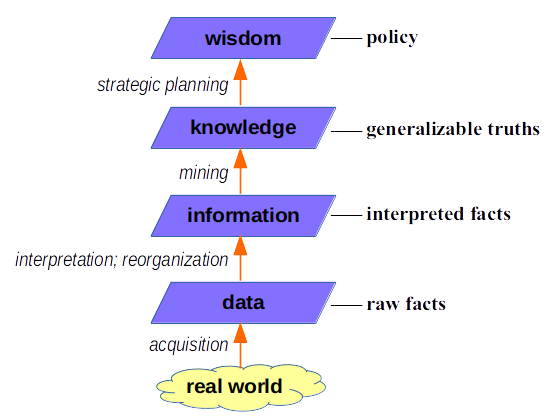
\includegraphics[width=0.9\textwidth]{dataHierarchy.png}
\caption{The data-to-wisdom hierarchy.}
\label{dataHierarchy}
\end{figure}

\subsection{The real world}
\index{real world}
\index{acquisition}

Ultimately, what we're interested in is not data, but aspects of the
\textbf{real world} -- album sales and video views, stock prices and employment
rates, hurricane trajectories and virus hot spots, or whatever. Data science
can't really get off the ground until some sort of \textbf{data acquisition}
takes place that records measurements of the real world in electronic form.

This sounds obvious, but it's important to keep in mind, actually. No matter
how much time we spend working with data, \textit{it's never the data that
actually matters -- it's the real-world phenomenon the data represents.} It
might seem strange to say that ``data'' is merely incidental to a data
scientist, but it's true. And I've definitely seen more than one data scientist
get so locked on to the data that they forget this basic truth.

One important observation is that decisions about exactly \textit{which} data
to acquire from the real world are often crucial in how things are interpreted
later on. To take an example close to home, let's say we're gathering
information on college professors so we can gauge which universities have the
highest performing faculty, and how this might be changing over the years. We
choose some representative set of criteria to measure for each faculty member
to get a rough assessment of their performance. Let's say we choose three
things: the number of research papers the professor publishes each year, the
total amount of research funding they've been granted, and the average student
evaluation score of the courses they teach. That seems like a good first cut at
assessing ``faculty performance.'' We then go on our merry data science way,
finding correlations, making data visualizations, and drawing conclusions.

This is all fine and dandy, provided we always keep in mind that it was those
three qualities, and \textit{only} those three, that we gathered in the first
place. If our study gains any traction, and university professors find they
have a vested interest in being ranked high in our yearly study, we'll discover
that they act to maximize \textit{only} the categories that are being
collected. We didn't gather data on how many university committees they served
on, or how many independent studies they supervised, or how many advisees they
had, \textit{etc.} Those metrics will inevitably become minimized in
importance, because they weren't part of what we lifted out of the real world
and onto the bottom rung of our lofty chain.

\index{GDP}
\index{Dow Jones Industrial Average}
\index{stock market}

The moral is: what we measure matters, often more than we realize. Our
country's GDP and the Dow Jones Industrial Average are easy things to quantify,
and so we often do. And thus they gain great importance in analyses of the
economy. But are they actually the most important indicators? Does focusing on
them leave out other, perhaps more vital, benchmarks? I'll just leave you with
that question for now.

\subsection{Data}

\index{gobbledy-gook}
\index{data}
\index{interpretation}

Have you ever gotten blood work done, say for an annual physical? I have. I
like to look over the numbers when the doctor hands me the results, just to
chuckle and wonder what they all mean. To me, a non-physician, they're all
pretty much gobbledy-gook. They tell me my TBC is 4.93 x10E6/$\mu$L, that
I have 5.7 Absolute Neutrophils, and a slightly out-of-range NT-proBNP (just
53.49 pg/mL, whatever the heck that means).

When I use the word \textbf{data} in the context of the hierarchy, this is what
I mean: recorded measurements, often (but not always) quantitative, that have
not yet been \textbf{interpreted}. They may be very precise, but they're also
quite meaningless without the context in which to understand them. They'd even
be meaningless to a \textit{physician} if I didn't provide the labels; try
telling your doctor that you have 4.93 ``something'' and see whether he/she
freaks out.

The good news is that when we're at the data stage of the hierarchy, we at
least have the stuff in an electronic form so we can start to \textit{do}
something with it. We also often make choices at this stage about how to
\textbf{organize} the data, choosing the appropriate type of atomic and/or
aggregate data structures that we'll discuss in detail in
Chapters~\ref{ch:atomicData} and beyond. This will allow us to bring our
analysis equipment to bear on the problem in powerful ways.

\subsection{Information}
\index{information}

Data becomes \textbf{information} when it \textit{informs} us of something;
\textit{i.e.}, when we know what it means. Getting large amounts of data
organized, formatted, and labeled the right way are jobs for the data
scientist, since turning that morass into useful knowledge is impossible
without those steps. When the aspects of the real world that we've collected
are properly structured and conceptually meaningful, we're in business.


\subsection{Knowledge}
\index{knowledge}
\index{generalizable truths}

Now \textbf{knowledge} is where the real action is. As shown in
Figure~\ref{dataHierarchy}, knowledge consists of \textit{generalizable}
truths.

\index{Chandra}
\index{Austin}
\index{bank teller}

Here's what I mean. Information is about specific individuals or occurrences.
When we say ``Chandra is a female bank teller, and earns \$48,000 a year,'' or
``Austin is a male bank teller, and earns \$69,000 a year,'' we have in our
information repository some individual facts. They can be looked up and
consulted when necessary, as you'll learn in the first part of this book.

But if we say ``women make less money than men do, even at the same jobs,''
we're in a different realm entirely. We have now generalized from specific
facts to more wide-reaching tendencies. In the language of our discipline,
we've moved from information to knowledge.

Properly gleaning knowledge from information is a trickier business than
interpreting individual data points. There are established rules, some of them
mathematical, for determining when an apparent pattern is actually reliable,
what kinds of relationships can be detected with data, whether a relationship
is causal, and so forth. We'll build some important foundations with this kind
of reasoning in this \textit{Crystal Ball} volume and its follow-on companion.
For now, I only want to make the point that \textit{knowledge} -- as opposed to
mere information -- opens up a whole new world of understanding. No longer is
the world limited to a chaotic collection of individual observations: we can
now begin to understand the general ways in which the world works...and perhaps
even to change them.

\subsection{Wisdom}
\index{wisdom}

\textbf{Wisdom} is the gold standard. It represents what we \textit{do} with
our knowledge. Let's say we indeed determine that on average men are paid
higher than women in our country, even for the same jobs. What do we do with
that realization? Is it okay? Do we want to try and fix it, and if so, how?
With laws? Education? Government subsidies? Revolution?

\index{simulation}
\index{uncertainty}

You'll remember my definition of Data Science on p.~\pageref{dsDefinition}:
deriving \textit{knowledge} from \textit{data}. This implies that the
``wisdom'' level of the hierarchy is really outside the discipline, and belongs
to other disciplines instead. And that's partially true: in some sense, the
data scientist's job stops when the deep truths about the real world are
ferreted out and illustrated, leaving it to CEOs, directors, and other policy
makers to act on them. But the data scientist is often involved here too, for a
simple reason: a decision maker wants to know what's likely to \textit{happen}
if a particular policy is implemented. Most non-trivial interventions will have
results that are hard to predict in advance, as well as unintended side
effects. One set of tools in the data scientist's toolkit is for making
principled, calculated predictions about such things, as well as quantifying
the level of \textbf{uncertainty} in the predictions. Sometimes, the technique
of \textbf{simulation} is used -- carrying out experiments on virtual societies
or systems to see the likely aggregate effects of different interventions. It's
like having a high-dimensional, multi-faceted crystal ball that lets you play
out various scenarios to their logical conclusions.

\bigskip

Starting with the rough and tumble real world and helping produce wise
decisions about how humankind can deal with it all: that's the grand promise of
the data science enterprise. And those are the mighty waters you're about to
dip your toes in! I hope you'll find it as exhilarating as I do.

% TODO: Applications (sports, Netflix, image recognition, Google, NLP,
% Coronavirus)


\section{A word of warning}

\index{Spiderman}

Before we dive into the nitty gritty, let me leave you with one more general
thought. It's actually an application of something Spiderman once said: ``with
great power comes great responsibility.''

\index{walking on water}

Here's the deal. The skills you'll learn in this book are so powerful and
(still!) so rare, that when you demonstrate them, people will think you can
walk on water. If you continue in the discipline, you'll become highly
sought-after (and well paid). People will constantly be asking you to work
with new data, to produce plots, predictions, and insights, and basically to do
your magic. You'll be treated as a guru: the oracle people go to when they want
the scoop.

This is ultra-cool, but also dangerous. Why dangerous? One simple reason:
because \textit{when you make a data-related claim, \textbf{people will believe
you.}} Pretty much unquestioningly. Most of your colleagues won't have the
expertise or understanding to double-check your snazzy results. And it wouldn't
occur to them to do that anyway -- after all, you're the wizard.

\index{uncertainty}

The truth of the matter is that data science lives on the knife edge of
\textbf{uncertainty}. With our crystal ball, we can make non-obvious assertions
about the past or present and even predict the future, but as with all
``knowledge,'' we must always hold it tentatively. We may be 95\% confident
that men are paid more than women...but that's only 95\% confidence, not 100\%.
We may have reason to believe that raising the minimum wage in a city will
decrease poverty by 3\%...but there's a 1 in 20 chance that it might decrease
it by as much as 6\%, or even \textit{increase} it by 1\%.

The abiding principle is that you should always be forthright about the limits
of your bold claims, the caveats behind your beautiful plots, and the level of
likelihood that your hypotheses will turn out to be wrong. Admittedly, doing so
will make you seem a little less magic. There are lots of talking heads on
television who deliberately \textit{obscure} the level of uncertainty in their
analyses so that they seem more certain (and more impressive) than they really
are. To be responsible data scientists, though, we're going to do the Spiderman
thing and be up front and transparent about exactly what we've found, and what
we might be missing.

Believe me, this will make you powerful enough!


\chapter{A trip to Jupyter}

\label{programmingEnvironment}
\index{execute}
\index{edit}
\index{language}
\index{environment!programming}
\index{programming environment}
Python is a ridiculously popular \textbf{language} for programming and data
science (currently the third most widely used in the world\footnote{See
\url{https://www.tiobe.com/tiobe-index/}.}) which is one of many reasons we're
using it for this course. The language itself is different from the
\textbf{programming environment} used to write code in it, just as ``English''
is different from ``Microsoft Word'' and ``Google Docs.'' A programming
environment is just a fancy name for a tool or application used to write
programs. At a minimum, it must include a way to \textbf{edit} (write and
revise) code, and a way to \textbf{execute} (run) it.

\index{Jupyter Notebooks}
\index{IDE}
\index{Spyder}
There are many different programming environments data scientists use to write
Python code, just as there are many different word processing apps people use
to write English. The choice largely comes down to personal preference. Some
use full-blown \textbf{IDE}s (``integrated development environments'') like
Spyder or Atom; some use text-based tools like Notepad++ or \texttt{vim}. In
this class, we're going to use the friendly and minimalistic ``\textbf{Jupyter
Notebooks}'' environment since it's appropriate for an intro experience.

\section{Jupyter Notebooks}

\index{cell}

The concept of a Jupyter Notebook is simple: it's a Web page with editable
``\textbf{cell}s.'' Each cell is a little text window you can type in.

\pagebreak
There are three kinds of cells in Jupyter Notebooks:
\vspace{-.15in}

\begin{description}
\index{cell!raw}
\item{\textbf{Raw.}} ``Raw'' is dumb. Never use it.
\index{Markdown}
\index{render}
\index{cell!Markdown}
\item{\textbf{Markdown.}} ``Markdown'' cells are for \textit{English text}, not Python
code. They're mostly used to describe and annotate what you're doing in the
code cells, like a running commentary. You can type plain-ol' text in a
Markdown cell, plus various cutesy formatting adornments like boldface (putting
double-splats (\texttt{**}) around a word or phrase), italics (single splats),
outline headings (prefacing a line with one or more hashtags (like \texttt{\#}
or \texttt{\#\#\#}), and so forth.\footnote{For a complete list of formatting
options, see
\url{https://github.com/adam-p/markdown-here/wiki/Markdown-Cheatsheet}.} When
you type in a Markdown cell, you see the raw text and formatting; to actually get Jupyter to
\textbf{render} your cells and make them pretty, you choose ``Run All'' from
the \index{run all@``Run All''} \index{cell menu@``Cell'' CoCalc menu} ``Cell'' menu.

\index{cell!Code}
\item{\textbf{Code.}} The most important cells are ``Code'' cells which contain (duh)
code. When executed (again, by choosing ``Run All'' from the ``Cell'' menu) they actually carry out
the Python instructions you have typed in that cell, and display any results.

\end{description}

By the way, a common snafu is to somehow accidentally click in a way that
changes the type of a cell from ``Code'' to one of the other types. If you do
this, the Python code in that cell won't execute until you change the type back
to ``Code'' (more on this below).

\index{cell!type dropdown}
\index{CoCalc}
Figure~\ref{fig:jupyterNotebook} shows a Jupyter Notebook hosted by the
\textbf{CoCalc} cloud computing platform, which we'll use this semester. It has
two cells, one Markdown and one Code. Note carefully the \textbf{cell-type
dropdown} which is kind of hidden in the middle of the page: it currently reads
``Code'' because the second cell is the one that's highlighted. (If we clicked
to highlight and edit the top cell, that dropdown would change to
``Markdown.'')

\begin{figure}[!h]
\centering
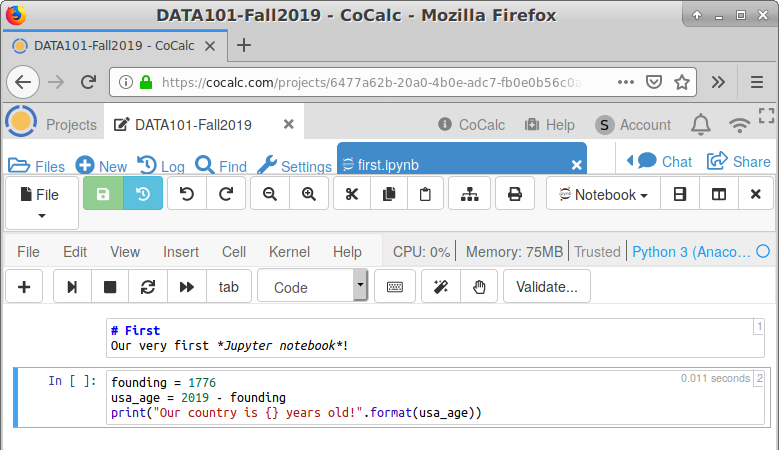
\includegraphics[width=0.85\textwidth]{firstNotebook.png} \\
\bigskip
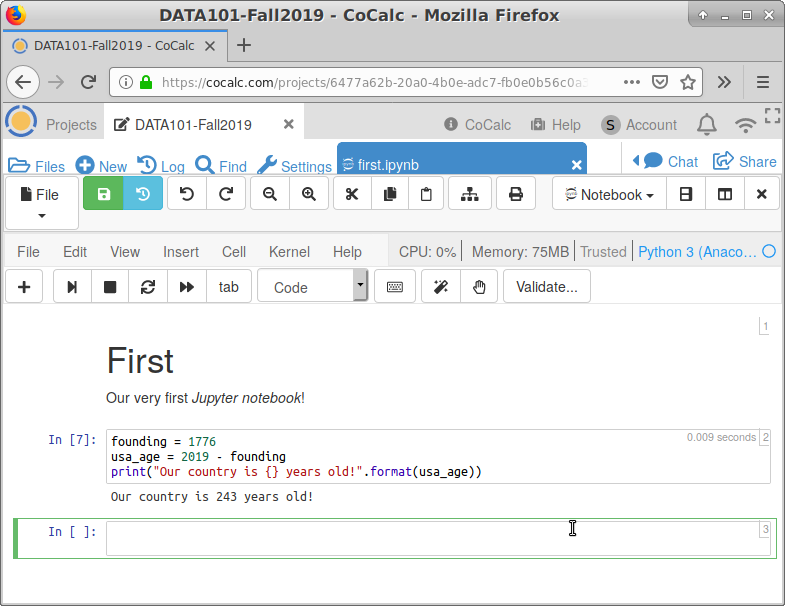
\includegraphics[width=0.85\textwidth]{firstNotebook2.png}
\medskip
\caption{A Jupyter Notebook with one Markdown cell and one Code cell. In the
top image, the two cells have been edited but not yet ``run'' -- hence
the Markdown formatting is unrendered and the code has not been executed. The
bottom pane shows both cells after the use has chosen ``Run All'' from the
``Cell'' menu.}
\label{fig:jupyterNotebook}
\end{figure}

\index{code snippet}
\index{snippet}
\index{output}
\index{*@\texttt{*} (splat)}
\index{splat}

The top figure shows the two cells before the user has done a ``Run All'' from
the ``Cell'' menu: all\index{run all@``Run All''} \index{cell menu@``Cell''
CoCalc menu} the Markdown is unrendered (see the literal splats and hashtags)
and the code is just sitting there. After ``Run All,'' the picture changes: you
see the formatted message in the top cell, and the \textbf{output} of the
Python code snippet after it runs. (The latter is easy to miss; stare at that
bottom picture and find the ``\texttt{Our country is 245 years old!}'' message.
That's the ``output.'') We haven't yet covered what that Python code means
(that's the main subject of this book) but you can probably guess some of what
it's doing.

%(Incidentally, you can see that when you Shift-Enter the bottom cell to run the
%code, Jupyter also creates a new empty cell at the end of the Notebook for you
%to type in. I find this annoying, but whatever.)

\section{Code and output}

Incredibly, that's about it. Everything else in this book is going to concern
what to type in those Code cells and how to interpret its output.

From now on, whenever I give example Python code in this book, I'll write it in
a box like this:

\begin{Verbatim}[fontsize=\small,samepage=true,frame=single,framesep=3mm]
founding = 1776
usa_age = 2021 - founding
print("Our country is {} years old!".format(usa_age))
\end{Verbatim}

That box means ``this stuff goes in a Code cell of a Notebook.''

When I write the corresponding output (\textit{i.e.}, what gets printed on the
page immediately below the code cell when ``Run All'' is chosen from the
``Cell'' menu), I'll write it like this:
\index{run all@``Run All''} \index{cell menu@``Cell'' CoCalc menu} 
\begin{Verbatim}[fontsize=\small,samepage=true,frame=leftline,framesep=5mm,framerule=1mm]
Our country is 245 years old!
\end{Verbatim}

That vertical bar means ``this stuff is the printed result of executing the
code cell.''

Easy enough. Onward!


% Other stuff I mentioned in class:
%
% For math, you think holistically. For programming, you think sequentially /
%   algorithmically.

\chapter{Three kinds of atomic data}
\label{ch:atomicData}

\section{Atomic data}

\index{atomic}
\index{indivisible}
When we say that some data is ``\textbf{atomic},'' we don't mean it's
radioactive; we mean it's \textit{indivisible}.

\index{Democritus}
\index{apple}
The ancients spoke of ``atoms'' as the smallest possible bits of matter. If you
divide up any physical object -- say, an apple -- into parts, you get its
components: a stalk, a stem, skin, seeds, and the sweet juicy stuff. Cut up any
of \textit{those} pieces with a knife and you get smaller pieces. If you
continue to split and split and split, philosophers like Democritus reasoned,
you'll eventually get to tiny indivisible bits that cannot be further
dissected. This is where the physical world bottoms out at the finest degree of
granularity.

Similarly, a piece of atomic data is typically treated as an entire unit, not
as something with internal structure that can be broken down. In the next
chapter we'll learn about various ways that these atoms of data can be strung
together and organized into larger wholes; for now, though, we're just looking
at the atoms themselves.

\section{Environments and variables}

\label{sec:envsAndVariables}
\index{environment}
\index{variable}
\index{variable!name}
\index{variable!value}
A data analysis program -- of which we will write many in this course -- makes
use of an \textbf{environment} as it runs. ``Environment'' just means ``all the
data that is currently in view, and which the program can
access.''\footnote{Confusingly, this use of the term ``environment'' is
different from the term ``programming environment'' I introduced on
p.\pageref{programmingEnvironment}.}  The environment consists of
\textbf{variables}, each of which (usually) has a \textbf{name} and a
\textbf{value}. For example, we might have a variable named \texttt{age} whose
value is 21, and a variable named \texttt{slogan} whose value is
\texttt{"Finger lickin' good"}.

\index{variable!name}
Each variable in the environment must have a \textit{distinct} name
(\textit{i.e.}, no two variables can share the same name). Also, importantly,
the reason these building blocks are called ``variables'' is that their value
can \textit{change} as the program executes. Although we may initially create
an \texttt{age} variable with the value \texttt{21}, later on in the program
the variable's value might change to \texttt{22}, or \texttt{50}, or
\texttt{0}. The variable's \textit{name} never changes, though.

\section{Atomic data types}

\index{variable!type}
There's one other thing that a variable has in addition to its name and value:
a \textbf{type}.\footnote{Strictly speaking, although in languages like Java
variables indeed have types, in Python the \textit{values} have types, not the
variables. This distinction will never be important for us though.}  In a
programming language like Python, every piece of data has a specific type,
which is necessary for determining how it behaves and what all you can do to
it. A question you should ask yourself a lot is: ``okay, I've got a variable in
my environment called \texttt{x}...now what is its type?'' You might have
guessed (correctly) that our \texttt{age} and \texttt{slogan} variables from
the previous section are of different types: one is a number, and the other is
a phrase.

In this course, we'll principally deal with three types of atomic data, all of
which will be familiar to you.


\subsection{Whole numbers}

\index{variable!whole number}
\index{whole number}
\index{likes@``likes''}
\index{votes}
One very common type of data is whole numbers, or integers. These are usually
positive, but can be negative, and have no decimal point. Things like a
person's birth year, a candidate's vote total, or a social media post's number
of ``likes'' are represented with this data type.


\subsection{Real (fractional) numbers}

\index{variable!real number}
\index{real number}
\index{fractional number}
\index{Facebook}
\index{movie rating}
\index{interest rate}
\index{temperature}
You may remember from high school math that the so-called ``real numbers''
include not only integers, but also numbers with digits after the decimal
point. This type can therefore be used to store interest rates, temperature
readings, and average movie ratings on a 1-to-5 scale.

Since all whole numbers are themselves real numbers, you might wonder why we
bother to define two different types for these. Why not just give both kinds of
variables the same real number type? Basically, the answer is that something
``feels wrong'' about that to the Data Science community. A Facebook user might
have 240 friends, or 241, but it would never make sense for her to have 240.3
friends. A consensus has thus arisen: variables that would only ever store
whole numbers really ought to be of a type that's devoted to only whole
numbers. You can violate this convention, but you'll be thought weird by your
fellow developers if you do so.


\subsection{Text}

\index{text}
\index{variable!text}
Lastly, some values obviously aren't numeric at all, like a customer's name, a
show title, or a tweet. So our third type of data is textual. Variables of this
type have a sequence of characters as values. These characters are most often
English letters, but can also include spaces, punctuation, and characters from
other alphabets.

\index{atomic}
\index{Avengers: Endgame@\textit{Avengers: Endgame}}
By the way, this third data type can tiptoe right up to the ``atomic'' line and
sometimes cross it. In other words, we will occasionally work with text values
\textit{non}-atomically, by splitting them up into their constituent words or
even letters. Most of the time, though, we'll treat a character sequence like
\texttt{"Avengers:\ Endgame"} as a single, indivisible chunk of data in the
same way we treat a number like \texttt{42}.

\subsection{But what about...?}

\index{song file}
\index{image file}
\index{video file}
What about other things a computer can store: images, song files, videos? It
turns out that through clever tricks, all these kinds of media and more can be
boiled down to a large number of integers, and stored in an aggregate data
structure like those discussed in the next chapter. At the atomic level, we'll
really only ever need to deal with the three types of this section.

\section{The three kinds in Python}

\index{language-general}
Now the three kinds of atomic data described above are
\textbf{language-general}: this means that they're conceptual, not tied to any
specific programming language or analysis tool. \textit{Any} technology used
for Data Science will have the ability to deal with those three basic types.
The specific ways they do so will differ somewhat from language to language.
Let's learn about how Python implements them.

\subsection{Whole numbers: \texttt{int}}

\index{int@\texttt{int}}
\index{integer}
One of the most basic Python data types is the ``\texttt{int},'' which stands
for ``integer.'' It's what we use to represent whole numbers.

\index{variable!value}
In Python, you create a variable by simply typing its name, an equals sign, and
then its initial value, like so:

\begin{Verbatim}[fontsize=\small,samepage=true,frame=single,framesep=3mm]
revolution = 1776
\end{Verbatim}

\index{line of code}
\index{code}
\index{executing@executing (code)}
\index{statement}
This is our first \textbf{line of code}\footnote{By the way, the word
\textbf{code} is grammatically a mass noun, not a count noun. Hence it is
proper to say ``I wrote some code last night,'' not ``I wrote some codes last
night.'' If you misuse this, it will brand you as a newbie right away.}. As
we'll see, lines of code are \textbf{executed} one by one -- there is a time
before, and a time after, each line is actually carried out. This will turn out
to be very important. (Oh, and a ``line of code'' is sometimes also called a
\textbf{statement}.)


\index{variable!name}
\index{underscore}
Python variable names can be as long as you like, provided they consist only of
upper and lower case letters, digits, and underscores. (You do have to be
consistent with your capitalization and your spelling: you can't call a
variable \texttt{Movie} in one line of code and \texttt{movie} in another.)
Underscores are often used as pseudo-spaces, but no other weird punctuation
marks are allowed in a variable's name.\footnote{Oh, and another rule: a
variable name can't \textit{start} with a digit. So \texttt{r2d2} is a legal
variable name, but not \texttt{007bond}.}

\index{movie rating}
\index{revolution@\texttt{revolution}}
And while we're on the subject, let me encourage you to \textit{name your
variables well}. This means that each variable name should reflect
\textit{exactly} what the value that it stores represents. Example: if a
variable is meant to store the rating (in ``stars'') that an IMDB user gave to
a movie, don't name it \texttt{movie}. Name it \texttt{rating}. (Or even
better, \texttt{movie\_rating}.) Trust me: when you're working on a complex
program, there's enough hard stuff to think about without confusing yourself
(and your colleagues) by close-but-not-exact variable names.\footnote{And I
fully own up to the fact that the \texttt{revolution} variable isn't named very
well. I chose it to make a different point shortly.}

\index{variable!type}
Now remember that a variable has three things -- a name, value, and type. The
first two explicitly appear in the line of code itself. As for the type, how
does Python know that \texttt{revolution} should be an ``\texttt{int}?''
Simple: it's \textit{a number with no decimal point.}

As a sanity check, we can ask Python to tell us the variable's type explicitly,
by writing this code:

\index{type@\texttt{type()}}
\label{typeFunction}
\begin{Verbatim}[fontsize=\small,samepage=true,frame=single,framesep=3mm]
type(revolution)
\end{Verbatim}

If this line of code is executed after the previous one is executed, Python
responds with:

\begin{Verbatim}[fontsize=\small,samepage=true,frame=leftline,framesep=5mm,framerule=1mm]
int
\end{Verbatim}

So there you go.

\index{code snippet}
\index{snippet}
Here's another ``\textbf{code snippet}'' (a term that just means ``some lines
of code I'm focusing on, which are generally only part of a larger program''):

\begin{Verbatim}[fontsize=\small,samepage=true,frame=single,framesep=3mm]
revolution = 1776
moon_landing = 1969
revolution = 1917
\end{Verbatim}

\index{revolution@\texttt{revolution}}
Now if this were a math class, that set of equations would be nonsensical. How
could the same variable (\texttt{revolution}) have two contradictory values?
But in a \textit{program}, this is perfectly legit: it just means that
immediately after the first line of code executes, \texttt{revolution} has the
value \texttt{1776}, and moments later, after the third line executes, its
value has changed to \texttt{1917}. Its value depends entirely on ``where the
program is'' during its execution.

\subsection{Real (fractional) numbers: \texttt{float}}

\index{float@\texttt{float}}
The only odd thing about the second data type in Python is its name. In some
other universe it might have been called a ``real'' or a ``decimal'' or a
``fractional'' variable, but for some bizarre historical reasons it is called a
\texttt{float}.\footnote{If you're curious, this is because in computer
programming parlance a ``floating-point number'' means a number where the
decimal point might be anywhere. With an integer like -52, the decimal point is
implicitly at the far right-hand side of the string of digits. But with numbers
like -5.2 or -.52 or -.000052 or even 520000, the decimal point has ``floated''
away from this fixed position.}

\index{decimal point}
All the same rules and regulations pertain to \texttt{float}s as they do to
\texttt{int}s; the only difference is you type a decimal point. So:

\begin{Verbatim}[fontsize=\small,samepage=true,frame=single,framesep=3mm]
GPA = 3.17
price_of_Christian_Louboutin_shoes = 895.95
interest_rate = 6.
\end{Verbatim}

\index{interest rate}
Note that the \texttt{interest\_rate} variable is indeed a \texttt{float} type
(even though it has no fractional part) because we typed a period:

\index{type@\texttt{type()}}
\begin{Verbatim}[fontsize=\small,samepage=true,frame=single,framesep=3mm]
type(interest_rate)
\end{Verbatim}
\begin{Verbatim}[fontsize=\small,samepage=true,frame=leftline,framesep=5mm,framerule=1mm]
float
\end{Verbatim}

\subsection{Text: \texttt{str}}

\index{string}
\index{str@\texttt{str}}
Speaking of weird names, a Python text variable is of type \texttt{str}, which
stands for ``\textbf{string}.'' You could think of it as a bunch of letters
``strung'' together like a beaded necklace.

\index{quotation marks}
\index{''@\texttt{\textquotesingle\textquotesingle} (ticks)}
\index{""@\texttt{\char`\"\char`\"} (quotes)}
Important: when specifying a \texttt{str} value, you must use \textbf{quotation
marks} (either single or double). For one thing, this is how Python tells that
you intend to create a \texttt{str} as opposed to some other type. Examples:

\index{lit}
\index{donut\_store@\texttt{donut\_store}}
\index{Paul's Bakery}
\begin{Verbatim}[fontsize=\small,samepage=true,frame=single,framesep=3mm]
slang = 'lit'
grade = "3rd"
donut_store = "Paul's Bakery"
url = 'http://umweagles.com'
\end{Verbatim}

\index{string!of digits}
\index{type@\texttt{type()}}
Notice, by the way, that a \textit{string of digits} is not the same as an
integer. To wit:

\begin{Verbatim}[fontsize=\small,samepage=true,frame=single,framesep=3mm]
schwarzenegger_weight = 249
action_movie = "300"

type(schwarzenegger_weight)
\end{Verbatim}
\begin{Verbatim}[fontsize=\small,samepage=true,frame=leftline,framesep=5mm,framerule=1mm]
int
\end{Verbatim}

\begin{Verbatim}[fontsize=\small,samepage=true,frame=single,framesep=3mm]
type(action_movie)
\end{Verbatim}
\begin{Verbatim}[fontsize=\small,samepage=true,frame=leftline,framesep=5mm,framerule=1mm]
str
\end{Verbatim}

See? The quotes make all the difference.

\subsubsection{The length of a string}

\index{string!length}
\index{len@\texttt{len()}}
We'll do many things with strings in this book. Probably the most basic is
simply to inquire as to a string's \textbf{length}, or the number of characters
it contains. To do this, we enclose the variable's name in parentheses after
the word \texttt{len}:

\begin{Verbatim}[fontsize=\small,samepage=true,frame=single,framesep=3mm]
len(slang)
\end{Verbatim}
\begin{Verbatim}[fontsize=\small,samepage=true,frame=leftline,framesep=5mm,framerule=1mm]
3
\end{Verbatim}

\begin{Verbatim}[fontsize=\small,samepage=true,frame=single,framesep=3mm]
len(donut_store)
\end{Verbatim}
\begin{Verbatim}[fontsize=\small,samepage=true,frame=leftline,framesep=5mm,framerule=1mm]
13
\end{Verbatim}

\label{function}
\index{lingo}
\index{function}
\index{argument}
\index{calling a function@``calling'' a function}
As we'll see, the \texttt{len()} operation (and many others like it) is an
example of a \textbf{function} in Python. In proper lingo, when we write a line
of code like \texttt{len(donut\_store)} we say we are ``\textbf{calling the
function},'' which simply means to invoke or trigger it.

\index{pass}
\index{passing an argument@``passing'' an argument}
\index{bananas (parentheses)}
\index{()@\texttt{()} (bananas)}
More lingo: for obscure reasons, the value inside the bananas
(here, \texttt{donut\_store}) is called an \textbf{argument} to the
function. And we say that we ``\textbf{pass}'' one or more arguments to a
function when we call it.

All these terms may seem pedantic, but they are precise and universally-used,
so be sure to learn them. The preceding line of code can be completely summed
up by saying:

\begin{quote}
``We are \textbf{calling} the \texttt{len()} \textbf{function},
and \textbf{passing} it the \texttt{donut\_store} \textbf{variable} as an
\textbf{argument}.''
\end{quote}

I recommend you say that sentence out loud at least four times in a row to get
used to its rhythm.

Note, by the way, that the \texttt{len()} function expects a \texttt{str}
argument. You can't call \texttt{len()} with an \texttt{int} or a
\texttt{float} variable as an argument:

\begin{Verbatim}[fontsize=\small,samepage=true,frame=single,framesep=3mm]
schwarzenegger_weight = 249

len(schwarzenegger_weight)
\end{Verbatim}

\begin{Verbatim}[fontsize=\small,samepage=true,frame=leftline,framesep=5mm,framerule=1mm]
TypeError: object of type 'int' has no len()
\end{Verbatim}

(You might think that the ``length'' of an \texttt{int} would be its number of
digits, but nope.)

\index{variable}
\index{variable!value}
One thing that students often get confused is the difference between a named
string \textit{variable} and that of an (unnamed) string \textit{value}.
Consider the difference in outputs of the following:

\begin{Verbatim}[fontsize=\small,samepage=true,frame=single,framesep=3mm]
slang = 'lit'
len(slang)
\end{Verbatim}
\begin{Verbatim}[fontsize=\small,samepage=true,frame=leftline,framesep=5mm,framerule=1mm]
3
\end{Verbatim}
\begin{Verbatim}[fontsize=\small,samepage=true,frame=single,framesep=3mm]
len('slang')
\end{Verbatim}
\begin{Verbatim}[fontsize=\small,samepage=true,frame=leftline,framesep=5mm,framerule=1mm]
5
\end{Verbatim}

In the first example, we asked ``how long is the value being held in the
\texttt{slang} variable?'' The answer was 3, since ``\texttt{lit}'' is three
characters long. In the second example, we asked ``how long is the word
\texttt{\textquotesingle slang\textquotesingle}?'' and the answer is 5. Remember: variable names never go in
quotes. If something is in quotes, it's being taken \textit{literally}.


\subsection{Combining and printing variables}

\index{printing a variable}
\index{print@\texttt{print()}}
There's a whole lot of stuff you can do with variables other than just creating
them. One thing you'll want to do frequently is \textbf{print} a variable,
which means to dump its value to the page so you can see it. This is easily
done by calling the \texttt{print()} function:

\begin{Verbatim}[fontsize=\small,samepage=true,frame=single,framesep=3mm]
print(donut_store)
print(price_of_Christian_Louboutin_shoes)
print("slang")
print(slang)
\end{Verbatim}

\begin{Verbatim}[fontsize=\small,samepage=true,frame=leftline,framesep=5mm,framerule=1mm]
Paul's Bakery
895.95
slang
lit
\end{Verbatim}

Again, don't miss the crucial difference between printing \texttt{"slang"} and
printing \texttt{slang}. The former is literal and the latter is not. In the
first of these, we're passing the \textit{word} ``\texttt{slang}'' as the
argument, not the variable \texttt{slang}.

\index{method}
Often we'll want to combine bits of information into a single print statement.
Typically one of the variables is a string that contains the overall message.
There are several ways to accomplish this, but the most flexible will turn out
to be the \texttt{.format()} \textbf{method}.

\index{calling a method@``calling'' a method (on a variable)}
\index{on@``on''}
I hate to hit you with so much new lingo. A \textbf{method} is very similar to
a function, but not exactly. The difference is in the syntax used to call it.
When you call a function (like \texttt{type()} or \texttt{len()}) you simply
type its name, followed by a pair of bananas inside of which you put the
arguments (separated by commas, if there's more than one). But when you ``call
a method,'' you put \textit{a variable} before a dot (``\texttt{.}'') and the
method name, then the bananas. This is referred to as ``calling the method
\textbf{on} the variable.''

It sounds more confusing than it is. Here's an example of \texttt{.format()} in
action:

\begin{Verbatim}[fontsize=\small,samepage=true,frame=single,framesep=3mm]
price_of_Christian_Louboutin_shoes = 895.95
message = "Honey, I spent ${} today!"
print(message.format(price_of_Christian_Louboutin_shoes))
\end{Verbatim}

\index{matching bananas}
\index{double bananas@``double bananas''}
Take note of how we write ``\texttt{message.format}'' instead of just
``\texttt{format}''. This is because \texttt{.format()} is a method, not a
function. We say that we are calling \texttt{.format()} ``on''
\texttt{message}, and passing \texttt{price\_of\_}\ \texttt{Christian\_Louboutin\_shoes}
as an argument.\footnote{Btw, in this book, whenever I refer to a method, I'll
be sure to put a dot before its name. For example, it's not the
``\texttt{format()}'' method, but the ``\texttt{.format()}'' method.} Also be
sure to notice the \textit{double} bananas ``\texttt{))}'' at the end of that
last line. We need both of them because in programming, every left-banana must
match a corresponding right-banana. Since we're calling two functions/methods
on one line (\texttt{print()} and \texttt{.format()}), we had two left-bananas
on that line. Each one needs a partner.

\index{\{\}@\texttt{\{\}} (curlies)}
As for the specifics of how \texttt{.format()} works, you'll see that the
string variable you call it on may include pairs of curlies (squiggly braces).
These are placeholders for where to stick the values of other variables in the
output. Those variables are then included as arguments to the
\texttt{.format()} method. The above code produces this output:

\begin{Verbatim}[fontsize=\small,samepage=true,frame=leftline,framesep=5mm,framerule=1mm]
Honey, I spent $895.95 today!
\end{Verbatim}

Often, instead of creating a new variable name to hold the pre-formatted
string, we'll just \texttt{print()} it literally, like this:

\begin{Verbatim}[fontsize=\footnotesize,samepage=true,frame=single,framesep=3mm]
print("Honey, I spent ${} today!".format(
    price_of_Christian_Louboutin_shoes))
\end{Verbatim}

We're still actually calling \texttt{.format()} on a variable here, it's just
that we haven't bothered to name the variable. Also, notice that our code was
too long to fit on one line nicely, so we broke it in two, and indented the
second line to make it clear that ``\texttt{price\_of\_}...'' wasn't
starting\index{bananas (parentheses)}\index{()@\texttt{()} (bananas)} its own new
line. Crucially, all the bananas are still paired up, two-by-two, even though
the left bananas are on a different line than the corresponding right bananas.

\bigskip
Finally, here's a longer example with more variables:

\begin{Verbatim}[fontsize=\footnotesize,samepage=true,frame=single,framesep=3mm]
name = "Pedro Pascal"
num_items = 3
cost = 91.73
print("Customer {} bought {} items worth ${}.".format(name,
    num_items, cost))
\end{Verbatim}

\begin{Verbatim}[fontsize=\small,samepage=true,frame=leftline,framesep=5mm,framerule=1mm]
Customer Pedro Pascal bought 3 items worth $91.73.
\end{Verbatim}

You can see how we can pass more than one argument to a function/method simply
by separating them with commas inside the bananas.


% TODO:
%   pow() function
%   .strip() string method
% memory diagrams -- diff between modifying in place and returning a copy (like
% .strip().)
% Left-side "variable names and atomic data". Right-side "aggregate data."

\chapter{Memory pictures}

Now that we've talked about the three important kinds of atomic variables,
let's consider the question of \textit{where they live}. It might sound like a
strange question. Aren't they ``in'' the Jupyter Notebook cell in which they
were typed?

Actually, no. And that brings me to the first mission-critical lesson of the
semester, which is a bane to all students who don't deeply grasp it. The lesson
is:

\begin{quote}
\textbf{The code itself is only a means to an end. The purpose of the code is
to read or write what's in memory.}
\end{quote}

\index{memory}
\index{environment}
\textbf{Memory} is the part of the computer in which variables and their values
are stored. To use the terminology of Chapter~\ref{ch:atomicData}, memory is
where the \textbf{environment} lives. It is \textit{invisible} to the
programmer, but it is also \textit{very much there.} The single most important
trick to learning how to write correct code is being able to summon to mind
what memory looks like at any point in time. The code you must write is a
natural consequence of that.

\section{A picture of memory}

\index{memory!picture}
It's easier with pictures at first, so we'll draw plenty of them. Our
\textbf{memory pictures} will have a very specific format, and this is
crucially important: don't get creative with how things are labeled or where
things are drawn. In order for your code to work \textit{you must have this
picture exactly right.} It's not art; it's science.

Our memory pictures will always be divided into exactly two ``realms,'' one on
the left and one on the right, labeled as follows:

\begin{center}

\includegraphics[width=.7\textwidth]{memoryPicture.png}
\end{center}

The left column's name should be recognizable, since that's exactly what we
covered last chapter. The right column won't have anything in it for a couple
chapters.

\subsection{Writing to memory}

When we create atomic variables in a Code cell, a la:

\begin{Verbatim}[fontsize=\small,samepage=true,frame=single,framesep=3mm]
pin_count = 844
username = 'Bekka Palmer'
\end{Verbatim}

each one gets put on the left-hand side of the diagram as a \textbf{named box}.
The name of the box is the variable's name, and the thing inside of the box is
its value.

\vspace{-.2in}
\begin{center}
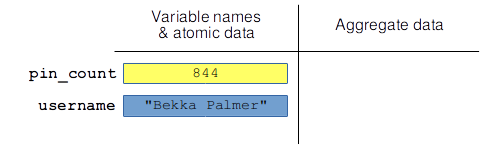
\includegraphics[width=.8\textwidth]{memoryPicture2.png}
\end{center}

It doesn't matter which boxes are higher or lower on the page, only that the
names stick with their boxes and don't get mixed up. As a bonus, I have colored
the boxes differently, indicating that \texttt{pin\_count} (an \texttt{int}) is
a different type than \texttt{username} (a \texttt{str}).\footnote{One other
tiny detail you might notice: even though our code had single quotes to delimit
Bekka Palmer's name, I put double quotes in the box in the memory picture. This
is to emphasize that no matter how you create a string in the code -- whether
with single quotes or double -- the underlying ``thing'' that gets written to
memory is the same. In fact, what's stored are actually the characters
\texttt{Bekka Palmer} \textit{without} the quotes. I like putting quotes in the
memory pictures, though, just to emphasize the string nature of the value.}

Creating more variables just adds more named boxes:

\begin{Verbatim}[fontsize=\small,samepage=true,frame=single,framesep=3mm]
...
avg_num_impressions = 1739.3
board_name = "Things to Make"
\end{Verbatim}

\vspace{-.2in}
\begin{center}
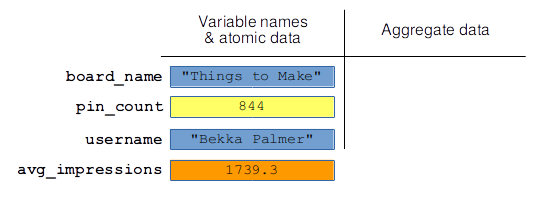
\includegraphics[width=.8\textwidth]{memoryPicture3.png}
\end{center}

I'm deliberately shuffling around the order of the boxes just to mess with you.
Python makes no guarantee of what ``order'' it will store variables in anyway,
and in reality it actually does become a big jumbled mess like this under the
hood. All Python guarantees is that it will consistently store a name, value,
and a type for each variable.

When we change the value of a variable (rather than creating a new one), the
value in the appropriate box gets updated:

\begin{Verbatim}[fontsize=\small,samepage=true,frame=single,framesep=3mm]
...
avg_num_impressions = 2000.97
pin_count = 845
another_board = 'Pink!'
\end{Verbatim}

\vspace{-.2in}
\begin{center}
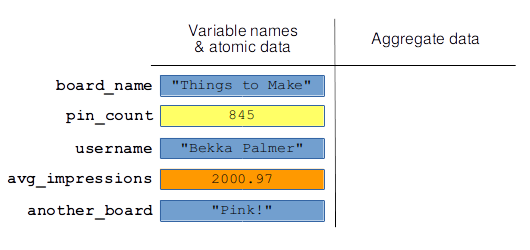
\includegraphics[width=.7\textwidth]{memoryPicture4.png}
\end{center}

Note carefully that \textit{the previous value in the box is completely
obliterated} and there is absolutely no way to ever get it back. There's no
way, in fact, to know that there even \textit{was} a previous value different
than the current one. Unless specifically orchestrated to do so, computer
programs only keep track of the present, not the past.

One other thing: unlike in some programming languages (so-called ``strongly
typed'' languages like Java or C++) even the \textit{type} of value that a
variable holds can change if you want it to. Even though the following example
doesn't make much sense, suppose we wrote this code next:

\begin{Verbatim}[fontsize=\small,samepage=true,frame=single,framesep=3mm]
...
pin_count = 999.635
username = 11
\end{Verbatim}

This causes not only the contents of the boxes to change, but even their
colors. The \texttt{username} variable was a \texttt{str} a moment ago, but now
it's an \texttt{int}.

\vspace{-.2in}
\begin{center}
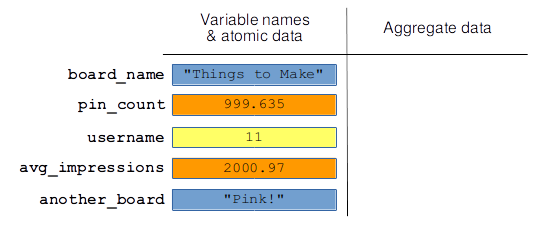
\includegraphics[width=.7\textwidth]{memoryPicture5.png}
\end{center}

\subsection{Reading from memory}

``Reading from memory'' just means referring to a variable in order to retrieve
its value. So far, we don't know how to do much with that other than print:

\begin{Verbatim}[fontsize=\small,samepage=true,frame=single,framesep=3mm]
print("The {} board has {} pins.".format(another_board, pin_count))
\end{Verbatim}

\begin{Verbatim}[fontsize=\small,samepage=true,frame=leftline,framesep=5mm,framerule=1mm]
The Pink! board has 999.635 pins.
\end{Verbatim}

The important point is that the memory picture is the (only) current, reliable
record of what memory looks like at any point in a program. Think of it as
reflecting a snapshot in time: immediately after some line of code executes --
and right before the following one does -- we can consult the picture to obtain
the value of each variable. This is exactly what Python does under the hood.

I stress this point because I've seen many students stare at complicated code
and try to ``think out'' what value each variable will have as it runs. That's
hard to do with anything more than a few lines. To keep track of
what-has-changed-to-what-and-when, you really need to maintain an up-to-date
list of each variable's value as the program executes...which is in fact
exactly what the memory picture is.

So if you're trying to figure out ``what will this program output if I print
the \texttt{odometer} variable immediately after line 12?'' don't stare at the
code and try to reconstruct its behavior from scratch. Instead, draw a memory
picture, update it accordingly as you walk through each line of code, and then
look at it for the answer.

\subsection{Tip}

By the way, investing in a small whiteboard and a couple of markers is a great
way to help you learn programming. They're perfect for drawing and updating
memory pictures as they evolve.

Hopefully this chapter was straightforward. These memory pictures will be
getting increasingly complex as we learn more kinds of things to store,
however, so stay sharp!


\chapter{Calculations}
\label{ch:calculations}

Our discipline obviously involves a lot of computation -- in fact, I expect the
first image that comes to mind when most people hear the words ``data science''
is one of numerical calculation. In this chapter, I'll lay out the Python
syntax for performing various mathematical operations on numbers, as well as
manipulating strings. These things appear in every program, and you'll find it
all straightforward.

And then I'll drop a bomb on you. I'll unveil a Python behavior which you'll
probably find completely unexpected, which flummoxes nearly every student who
first sees it, and yet which you must understand and master to succeed in
Python or any programming language.

\section{Mathematical operations}

\index{operator}

\index{bananas (parentheses)}
\index{()@\texttt{()} (bananas)}
\index{curlies (curly braces)}
\index{\{\}@\texttt{\{\}} (curlies)}
\index{boxies (square brackets)}
\index{[]@\texttt{[]} (boxies)}
\index{wakkas (angle brackets)}
\index{<>@\texttt{<>} (wakkas)}
\index{+@\texttt{+}}
\index{-@\texttt{-}}
\index{/@\texttt{/}}
\index{**@\texttt{**}}
First, the easy part. Python has a number of built-in \textbf{operators} to do
the familiar math stuff. Figure~\ref{fig:mathOps} has a table of the ones we'll
use. A few are mildly surprising (\texttt{*} instead of \texttt{X} for
multiplication; \texttt{/} instead of $\div$ for division, which I'll bet you
couldn't find on your keyboard anyway), and you have to remember to use only
bananas (not boxies \texttt{[]}, curlies \texttt{\{\}}, or wakkas \texttt{<>})
for grouping sub-expressions within a larger expression. Otherwise, it's a
piece of cake.

\begin{figure}[ht]
\centering
\begin{tabular}{c | l}
\hline
Operator & Operation \\
\hline
\texttt{+} & addition \\
\texttt{-} & subtraction \\
\texttt{*} & multiplication \\
\texttt{/} & division \\
\texttt{**} & exponentiation (``to the power of'')\\
\texttt{()} & grouping \\
\hline
\end{tabular}
\smallskip
\caption{Python's basic math operators.}
\label{fig:mathOps}
\end{figure}

All this stuff has to appear on the \textbf{right-hand side} of an equals sign,
by the way, never on the left. That may seem surprising, since in mathematics
the equations ``$x = y + 3$'' and ``$y + 3 = x$'' mean the same thing. Why does
it matter which order you write it in? The answer, you'll recall, is that in a
program the symbol ``\texttt{=}'' doesn't mean ``\textit{is} equal to'' but
rather ``\textit{make} equal to.'' It's not an equation; it's a command. And
you can't command ``$y+3$'' to be equal to anything. Therefore the only thing
permitted on the left-hand side of an equals sign is a single, plain-jane
variable name.

To test your understanding of the syntax, see if you agree that the following
math expression:

\begin{align*}
\textrm{gpa} = \frac{
\textrm{creds}_1 \cdot \textrm{gpts}_1 +
\textrm{creds}_2 \cdot \textrm{gpts}_2}
{\textrm{creds}_1 + \textrm{creds}_2}
\end{align*}

should look like this in Python:

\begin{Verbatim}[fontsize=\footnotesize,samepage=true,frame=single,framesep=3mm]
gpa = (creds1 * gpts1 + creds2 * gpts2) / (creds1 + creds2)
\end{Verbatim}

and that this one:

\begin{align*}
a = \frac{\lbrack x^2y(4-z) + (x+q)\cdot y \rbrack \times 2^{15y+2z}}
{19x^3 - (yz)^{(y-1)^2}}
\end{align*}

should look like this:

\begin{Verbatim}[fontsize=\tiny,samepage=true,frame=single,framesep=3mm]
a = (((x**2)*y*(4-z) + (x+q)*y) * 2**(15*y+2*z)) / (19*(x**3) - (y*z)**((y-1)**2))
\end{Verbatim}

\vspace{-.15in}

If so, you're good to go. It's tedious, but not complicated.

Python also has plenty of functions for absolute value, sine and cosine,
logarithms, square roots, and anything else you can think of. We'll learn all
those at the proper time (or they're all eminently Google-able if you want to
look them up now).

\subsection{A common pattern: cumulative totals}

\label{cumulativeTotal}
\index{cumulative total}

Here's a technique we'll use over and over in our code, but which can seem a
bit jarring the first time you see it. Check out this line of code:

\begin{Verbatim}[fontsize=\small,samepage=true,frame=single,framesep=3mm]
balance = balance + 50
\end{Verbatim}

Now there is no universe where that statement is true \textit{mathematically}.
(Think about it: can you come up with any number that is equal to itself plus
fifty? I thought not.) But again, this is programming, not algebra. We're
\textit{commanding} the \texttt{balance} variable to have a new value. And what
is that new value? Simple: whatever its \textit{previous} value was, plus 50.

The net effect is to increase \texttt{balance}'s value by 50. Follow this:

\begin{Verbatim}[fontsize=\small,samepage=true,frame=single,framesep=3mm]
balance = 1000
print("In July, I had ${}.".format(balance))
balance = balance + 50
print("In August, I had ${}.".format(balance))
balance = balance - 200
balance = balance + 120
print("In September, I had ${}.".format(balance))
\end{Verbatim}
\vspace{-.2in}

\begin{Verbatim}[fontsize=\small,samepage=true,frame=leftline,framesep=5mm,framerule=1mm]
In July, I had $1000.
In August, I had $1050.
In September, I had $970.
\end{Verbatim}

\index{loop}

You get the idea. This approach will become especially useful when we get to
\textbf{loops} in Chapter~\ref{ch:loops}, because we'll be able to repeatedly
\textbf{increment} a variable's value by a desired amount in automated fashion.

\medskip

\index{increment}
\index{counter variable}
A couple other things. First, a very common special case of the above is to
increment a variable by exactly \textit{one}:

\vspace{-.15in}
\begin{Verbatim}[fontsize=\small,samepage=true,frame=single,framesep=3mm]
number_of_home_runs = number_of_home_runs + 1
\end{Verbatim}
\vspace{-.15in}

This allows us to count the occurrences of various things: every time somebody
hits a home run (or whatever), the above line of code will increase the
appropriate \textbf{counter variable}'s value by one.

\smallskip

Second, Python has a special alternative syntax for this incrementing
operation. It looks weird:

\vspace{-.15in}
\begin{Verbatim}[fontsize=\small,samepage=true,frame=single,framesep=3mm]
balance += 50
number_of_home_runs += 1
\end{Verbatim}

\index{+=@\texttt{+=} (``plus-equals'')}
\index{plus equals@``plus-equals'' (\texttt{+=})}
The two characters ``\texttt{+}'' and ``\texttt{=}'' (pronounced
``plus-equals'') allow us to shorthand this operation and avoid typing the
variable name twice. The above two lines of code are \textit{exact} synonyms
for these:

\vspace{-.15in}
\begin{Verbatim}[fontsize=\small,samepage=true,frame=single,framesep=3mm]
balance = balance + 50
number_of_home_runs = number_of_home_runs + 1
\end{Verbatim}

You can use whichever one you wish, although be aware that your fellow
programmers may well choose the former one, so you need to understand what it
means.

\section{String operations}

\index{trimming@trimming (a string)}
\index{whitespace}
\index{tacking on (concatenating) strings}
\index{concatenating!strings}
\label{concatenatingStrings}
\index{+@\texttt{+}}
\index{case@case (upper and lower)}
Text data, too, has many things that can be done to it. For now, let's just
learn a few techniques for \textbf{concatenating} strings (tacking one onto the
end of another) \textbf{trimming} strings (removing
\textbf{whitespace}\footnote{The word ``whitespace'' is a catch-all for spaces,
tabs, newline characters, and most anything else invisible.} from the ends) and
changing their \textbf{case} (upper/lower). See Figure~\ref{fig:stringOps} for
a list.

\index{lstrip@\texttt{.lstrip()}}
\index{rstrip@\texttt{.rstrip()}}
\index{strip@\texttt{.strip()}}
\index{upper@\texttt{.upper()}}
\index{lower@\texttt{.lower()}}
\index{title@\texttt{.title()}}

\begin{figure}[ht]
\small
\centering
\begin{tabular}{c | l}
\hline
Method/operator & Operation \\
\hline
\texttt{+} & concatenate two strings \\
\texttt{.lstrip()} & remove leading whitespace \\
\texttt{.rstrip()} & remove trailing whitespace \\
\texttt{.strip()} & remove leading and trailing whitespace \\
\texttt{.upper()} & convert to all uppercase \\
\texttt{.lower()} & convert to all lowercase \\
\texttt{.title()} & convert to ``title case'' (capitalize each word) \\
\hline
\end{tabular}
\smallskip
\caption{A few of Python's string methods.}
\label{fig:stringOps}
\end{figure}

The plus sign is an operator, like the mathematical ones in
Figure~\ref{fig:mathOps}: it's used to concatenate (append) one string to
another. Example:

\begin{Verbatim}[fontsize=\small,samepage=true,frame=single,framesep=3mm]
x = "Lady"
y = "Gaga"
z = x + y
print(z)
\end{Verbatim}

\begin{Verbatim}[fontsize=\small,samepage=true,frame=leftline,framesep=5mm,framerule=1mm]
LadyGaga
\end{Verbatim}

The second one is slapped right on the end of the first; there's no spaces or
punctuation. If you wanted to insert a space, you'd have to do that explicitly
with a string-that-consists-of-only-a-space (written as the three characters:
quote, space, quote), like this:

\begin{Verbatim}[fontsize=\small,samepage=true,frame=single,framesep=3mm]
first = 'Dwayne'
last = "Johnson"
full = first + ' ' + last
print(full)
\end{Verbatim}

\begin{Verbatim}[fontsize=\small,samepage=true,frame=leftline,framesep=5mm,framerule=1mm]
Dwayne Johnson
\end{Verbatim}

Punctuation marks, too, have to be included literally, and it can be tricky to
get everything typed in the right way:

\begin{Verbatim}[fontsize=\small,samepage=true,frame=single,framesep=3mm]
first = 'Dwayne'
last = "Johnson"
nick = 'The Rock'
full = first + ' "' + nick + '" ' + last
print("Don't ya just love {}?".format(full))
\end{Verbatim}

\begin{Verbatim}[fontsize=\small,samepage=true,frame=leftline,framesep=5mm,framerule=1mm]
Don't ya just love Dwayne "The Rock" Johnson?
\end{Verbatim}

Stare at that line beginning with ``\texttt{full =}'' and see if you can figure
out why each punctuation mark is where it is, and why there are spaces between
some of them and not between others.

By the way, here's a bit of a head-scratcher at first:

\begin{Verbatim}[fontsize=\small,samepage=true,frame=single,framesep=3mm]
matriculation_year = "2021"
graduation_year = matriculation_year + 4
print("Imma graduate in {}!".format(graduation_year))
\end{Verbatim}

\begin{Verbatim}[fontsize=\small,samepage=true,frame=leftline,framesep=5mm,framerule=1mm]
Imma graduate in 20214!
\end{Verbatim}

Whoa -- wut? That's a lot of tuition. The problem here is that
\texttt{matriculation\_year} was defined as a \textit{string}, not an integer
(note the quotes). So the \texttt{+} sign meant concatenation, not addition.
Remember: a string-consisting-only-of-digits is not the same as a number. (If
you remove the quotes from the first line, your mom will breathe easier and
you'll get the result you expect.)

The other items in Figure~\ref{fig:stringOps} are methods: they have an initial
dot (``\texttt{.}'') and they must be called ``\textbf{on} a string'' (meaning,
a string variable name must immediately precede them). They also take no
arguments, which means that a lonely, empty pair of bananas comes after their
name when they are called. Examples:

\index{Carl's Ice Cream}
\begin{Verbatim}[fontsize=\small,samepage=true,frame=single,framesep=3mm]
shop_title = "               carl's ICE cream      "
print(shop_title)
print(shop_title.strip())
print(shop_title.upper())
print(shop_title.lower())
print(shop_title.title())
\end{Verbatim}

\begin{Verbatim}[fontsize=\small,samepage=true,frame=leftline,framesep=5mm,framerule=1mm]
               carl's ICE cream         
carl's ICE cream
               CARL'S ICE CREAM         
               carl's ice cream         
               Carl'S Ice Cream         
\end{Verbatim}

(You can't see the trailing spaces in the output, but you can see the leading
ones.)

You can even combine method calls back to back like this:

\begin{Verbatim}[fontsize=\small,samepage=true,frame=single,framesep=3mm]
print(shop_title.strip().upper())
\end{Verbatim}

\begin{Verbatim}[fontsize=\small,samepage=true,frame=leftline,framesep=5mm,framerule=1mm]
Carl'S Ice Cream
\end{Verbatim}

\index{data cleansing}
These operations are for more than mere prettiness. They're also used for
\textbf{data cleansing}, which is often needed when dealing with messy,
real-world data sets. If, say, you asked a bunch of people on a Web-based
survey which Fredericksburg ice cream store they prefer, lots of them will name
Carl's: but they'll type the capitalization every which way, forget the
apostrophe, clumsily add spaces to one end (or even both, or even in the
middle), yet they'll all have in mind the same luscious vanilla cones. One step
towards conflating all these different expressions to the same root answer
would be trimming the whitespace off the ends and converting everything to all
lower-case. More surgical operations like removing punctuation or spaces in the
middle is a bit trickier; stay tuned.

\section{Return values}

\label{returnValues}
\index{bomb}
Okay, you've been in suspense long enough. Time for the bomb.

\index{calling a function@``calling'' a function}
\index{passing an argument@``passing'' an argument}
First, we're going to add another phrase to our already lengthy
function-calling mantra. You'll recall that we summarized this code (a function
call):

\begin{Verbatim}[fontsize=\small,samepage=true,frame=single,framesep=3mm]
len(movie_title)
\end{Verbatim}

with this English:

\begin{quote}
``We are calling the \texttt{len()} function, and passing it
\texttt{movie\_title} as an argument.''
\end{quote}

\index{calling a method@``calling'' a method (on a variable)}
\index{on@``on''}
And we summarized this code (a method call):

\begin{Verbatim}[fontsize=\small,samepage=true,frame=single,framesep=3mm]
message.format(name, age)
\end{Verbatim}

with this English:

\begin{quote}
``We are calling the \texttt{.format()} method \textbf{on} the \texttt{message}
variable, and passing it \texttt{name} and \texttt{age} as arguments.''
\end{quote}

\index{return value}
\index{output!of a function}
\index{return@``returning'' a value}
Now, a third thing. We can use the equals sign with a variable name to
capture the output of the function or method, instead of just printing it. The
output of a function is called its \textbf{return value}. We say that ``the
\texttt{.upper()} method \textbf{returns} an upper-case version of the string
it was called \textbf{on}.'' We can capture it like this:

\begin{Verbatim}[fontsize=\small,samepage=true,frame=single,framesep=3mm]
big_and_loud = shop_title.upper()
\end{Verbatim}

The variable \texttt{big\_and\_loud} now holds the value
\texttt{"CARL\textquotesingle S ICE CREAM"}. Functions work similarly:

\begin{Verbatim}[fontsize=\small,samepage=true,frame=single,framesep=3mm]
width_of_sign = len(shop_title)
\end{Verbatim}

The \texttt{width\_of\_sign} int now has the value 40 (remember all those
extraneous spaces); if we'd trimmed first, we'd have gotten 16:

\begin{Verbatim}[fontsize=\small,samepage=true,frame=single,framesep=3mm]
true_width_of_sign = len(shop_title.strip())
print(true_width_of_sign)
\end{Verbatim}

\begin{Verbatim}[fontsize=\small,samepage=true,frame=leftline,framesep=5mm,framerule=1mm]
16
\end{Verbatim}


\subsection{The bomb}

I've probably built this up too much, but I think you'll agree that the
following output is pretty surprising:

\begin{Verbatim}[fontsize=\small,samepage=true,frame=single,framesep=3mm]
diva = "Ariana Grande"
diva.upper()
print("I just love {}!".format(diva))
\end{Verbatim}

\begin{Verbatim}[fontsize=\small,samepage=true,frame=leftline,framesep=5mm,framerule=1mm]
I just love Ariana Grande!
\end{Verbatim}

Wait...did the ``\texttt{diva.upper()}'' part just not work? Did it get
skipped? Did we do it wrong somehow?

Even more confusing, putting the ``\texttt{.upper()}'' call directly in the
\texttt{print} statement seems to work...but only temporarily. Accessing
\texttt{diva} a moment later appears to revert it back to its old value:

\begin{Verbatim}[fontsize=\small,samepage=true,frame=single,framesep=3mm]
diva = "Ariana Grande"
print("I just love {}!".format(diva.upper()))
print("When does the next {} album come out?".format(diva))
\end{Verbatim}

\begin{Verbatim}[fontsize=\small,samepage=true,frame=leftline,framesep=5mm,framerule=1mm]
I just love ARIANA GRANDE!
When does the next Ariana Grande album come out?
\end{Verbatim}

The root cause of this and practically all perplexing Python printing can be
discovered by consulting the memory picture. Here's how it starts out when we
first define \texttt{diva}:

\vspace{-.2in}
\begin{center}
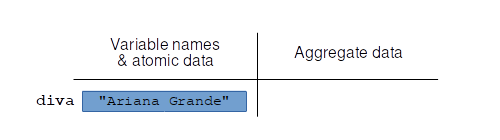
\includegraphics[width=0.9\textwidth]{bomb.png}
\end{center}

Now say we do this:

\begin{Verbatim}[fontsize=\small,samepage=true,frame=single,framesep=3mm]
new_var_name = diva.upper()
\end{Verbatim}

The result is this picture:

\vspace{-.2in}
\begin{center}
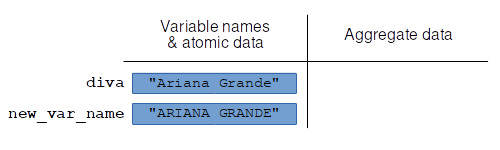
\includegraphics[width=0.9\textwidth]{bomb2.png}
\end{center}

And now we see the reason for it all. The contents of the \texttt{diva}
variable itself are \textit{\textbf{unchanged}} by the method call. Calling
``\texttt{.upper()}'' on \texttt{diva} didn't change the string value in
\texttt{diva}: it merely \textit{returned} a modified \textit{copy} of the
string.

Think of it this way: if I asked you, ``what is your name in Pig Latin?'' and
you told me, that would not intrinsically \textit{change} your actual name to
be in Pig Latin. You would simply be ``returning'' to me the Pig Latin version
of it in response to my query.

You could argue this behavior of Python's is dumb, or at best misleading, and
I'm actually inclined to agree with you in this case. But of course beggars
can't be choosers: someone took the time to write the \texttt{.upper()} method
for us, so if we want to take advantage of it we have to use his/her owner's
manual. And the fact is that many (perhaps even most) Python functions/methods
-- including many of the ones from Pandas, which we'll use extensively -- are
coded with this style: not actually modifying the variables they are passed,
but instead returning to you a modified copy which you must store.

Now given that this is the case, it would at least be nice if I could tell you
that it always, consistently worked this way. Then you could simply accept it
and get used to it. Alas, no. There \textit{are} functions/methods (lots of
them) which \textit{do} modify a parameter or the variable they were called on.
So sometimes, our na\"{i}ve approach of calling the method and expecting the
variable to change is exactly what we need to do. The bottom line is:
\textit{there's no way of knowing without being told, or else reading the
documentation.} We'll learn how to do the latter in a future chapter. For now,
I'm simply telling you for the record that the methods in
Figure~\ref{fig:stringOps} are all of the ``return a modified copy'' type, and
giving you a heads up that both styles of method do exist out there in
abundance.

A couple more things. First, as a corollary of the above, realize that the
following statement (on a line by itself) is officially 100\% useless:

\begin{Verbatim}[fontsize=\small,samepage=true,frame=single,framesep=3mm]
name_of_pet.lstrip()
\end{Verbatim}

You called the \texttt{.lstrip()} method, and then....did nothing with the
return value. If you don't store it in a variable -- or else do something with
it right away like \texttt{print} it before it slips out of your fingers --
it's irrevocably lost: it doesn't even show up on the memory picture because
there's no variable name. (Think about that.)

Second, note the following pattern which is very often used:

\begin{Verbatim}[fontsize=\small,samepage=true,frame=single,framesep=3mm]
name_of_pet = name_of_pet.lstrip()
\end{Verbatim}

Here, we're calling \texttt{.lstrip()} on the \texttt{name\_of\_pet} variable
\textit{and then storing the return value back in the \texttt{name\_of\_pet}
variable}. This might be what you thought would have happened in the first
place -- the author of the previous, useless line, probably wanted the variable
itself to permanently have its leading spaces removed. Simply calling
\texttt{.lstrip()} on the variable won't do that, but putting the revised value
back in the same blue box on the memory diagram will.


% note that "variable" means something different in this chapter. Not a single
% value, but multiple measurements.

\chapter{Scales of measure}

In the last chapter, we learned the Python verbiage for how to do arithmetic
operations. In this one, we zoom out and ask: when does it actually make
\textit{sense} to use those operations? The answer turns out to be: not always.

\index{syntax}
\index{semantics}
\index{meaning}
Another way to phrase this distinction is in terms of \textbf{syntax}
vs.~\textbf{semantics}. Syntax concerns the rules for combining various symbols
in a programming (or other) language. Semantics concerns the \textit{meaning}
of those symbols. This isn't something a programming language can tell us. Only
a human who understands what all those symbols refer to can determine when a
particular combination actually relates to something meaningful. Let this
chapter be your guide.

\index{scales of measure}
\section{The four scales of measure}

Every variable we collect can have various values, and the nature of
information it contains can be described by its \textbf{scale of measure}.
There are four of these\footnote{According to psychologist Stanley Smith
Stevens in 1946. Other researchers have developed related, but different,
scales of measure.}, and each one determines which kinds of operations are
``legal'' (\textit{i.e.}, sensible) with that variable.

\index{categorical variable}
\index{nominal variable}
\subsection{Categorical/nominal}

The first one is the simplest, although it actually has two different names in
common use: \textbf{categorical} or \textbf{nominal} variables. It is the scale
of variables that represent ``one of a set of choices,'' where no choice is
``higher'' or ``greater'' than any other.

\index{order}
An example would be a \texttt{fave\_color} variable that holds the value of a
child's favorite color: legal values are \texttt{"red"}, \texttt{"blue"},
\texttt{"green"} or \texttt{"yellow"}. We know it's categorical from, among
other things, the fact that there's no one right way to \textbf{order} those
values. (Alphabetical, most-popular-first, and ordering according to the
sequence of the rainbow are three possibilities. You might think of others.)

Political affiliation would be another categorical variable. Its values (like
\texttt{"Democrat"}, \texttt{"Republican"}, and \texttt{"Green"}) aren't in any
particular order. (Although you might think of the traditional left-to-right
political spectrum, that's only one dimension of political party, and perhaps
not even the most important one.) Other examples include film's genre, a
student's nationality, and a football player's position.

Now you might be tempted to think, ``hmm...all the categorical examples so far
are textual, not numeric. Perhaps this scales of measure thing is just another
way of stating the variable type?'' Alas, no. For one, we'll see text variables
in the next category as well. For another, even data that on its surface seems
numeric can actually be categorical in disguise.

Consider the uniform number of an athlete. I might be interested in asking,
``which uniform number had the greatest professional athletes who chose it?''
24 is a good candidate: Willie Mays, Ken Griffey Jr., and Kobe Bryant all wore
that jersey number. Or maybe \#7 is the winner, with Mickey Mantle, John Elway,
and Cristiano Ronaldo. Either way, though, all that matters in this analysis is
\textit{which} uniform number an athlete chose, not ``how high'' or ``how
great'' that number is compared to others. No one in their right mind would say
that Peyton Manning (\#18) was ``twice the player'' Mia Hamm was (\#9), because
uniform numbers aren't really ``numbers'' at all: they're more like labels.

\subsubsection{Legal operations for categorical/nominal variables}

\index{mode}
\index{central tendency}
\index{measure of central tendency}
When a variable is on a categorical scale, about the only things you can do are
compare for equality/inequality, count the occurrences of different values, and
compute something called the \textbf{mode} of the set.

The mode simply means the value that occurs \textit{the most often}. It's the
first of the ``\textbf{measures of central tendency}'' we'll see: such measures
are a way of capturing something about the ``typical'' value of a variable. For
categorical variables, the only typical-ness is ``which one occurs the most
often?'' If we ask a bunch of people for their \texttt{fave\_color}, and we get
the answers \texttt{"blue"}, \texttt{"red"}, \texttt{"blue"}, \texttt{"blue"},
and \texttt{"yellow"}, then the mode is \texttt{"blue"}. It's that simple.

To wrap things up, these things make sense to ask of a \textit{categorical}
variable:

\begin{compactitem}
\item[\leftthumbsup] ``Is his favorite color the same as her favorite color?''
\item[\leftthumbsup] ``How many people have \texttt{"red"} as their favorite
color?''
\item[\leftthumbsup] ``What's the most popular favorite color?''
\end{compactitem}

while these do \textit{not}:

\begin{compactitem}
\item[\leftthumbsdown] ``Is his favorite color greater than her favorite
color?'' (??)
\item[\leftthumbsdown] ``What's Caitlin's favorite color minus Hannah's?'' (??)
\item[\leftthumbsdown] ``What's the `average' favorite color in this data
set?'' (??)
\end{compactitem}


\index{ordinal variable}
\index{order}
\subsection{Ordinal}

One step up on the food chain is an \textbf{ordinal} variable, which means that
its different possible values \textit{do} have some meaningful order.

Consider \texttt{education\_level}, a variable that contains the highest degree
a survey respondent has earned. Its values can be any of the following:
\texttt{"HS"}, \texttt{"Associates"}, \texttt{"Bachelors"}, \texttt{"Masters"},
and \texttt{"PhD"}. In some ways, this is like \texttt{fave\_color}: the
variable must take on one of a set of specific, prescribed values. However,
it's pretty clear that a High School degree is closer to (more similar to) an
Associates degree than it is to a Ph.D. Each successive value represents more
education, and so unlike categorical variables, it \textit{does} make sense to
compare them along greater-than-or-less-than lines.

In addition to the mode, another measure of central tendency available for
ordinal variables is the \textbf{median}. I think of the median as the
``middlest'' value: if you line up all the occurrences in a row -- in order of
the values -- it's the one that lies in the exact middle. Suppose our survey
respondents give these answers: \texttt{"Bachelors"}, \texttt{"HS"},
\texttt{"HS"}, \texttt{"Masters"}, \texttt{"Masters"}, \texttt{"Bachelors"},
and \texttt{"HS"}. To compute the median, we line them all up in order:

\begin{center}
\texttt{"HS"  "HS"  "HS"  "Bachelors"  "Bachelors"  "Masters"  "Masters"}
\end{center}

nd find the middlest one, which is \texttt{"Bachelors"}. So \texttt{"HS"} is
the mode of this variable, and \texttt{"Bachelors"} is the median.

Other examples of ordinal variables include an NCAA basketball team's top-25
ranking, a taxpayer's tax bracket, and survey questions asking whether you
\texttt{"strongly disagree"}, \texttt{"disagree"}, are \texttt{"neutral"},
\texttt{"agree"}, or \texttt{"strongly agree"} with a certain statement.

Again, a list. For \textit{ordinal} variables, these are okay:

\begin{compactitem}
\item[\leftthumbsup] ``Is his education level the same as her education level?''
\item[\leftthumbsup] ``How many people answered \texttt{"strongly disagree"} to
this question?''
\item[\leftthumbsup] ``Is UMW basketball ranked higher or lower than Messiah?''
\item[\leftthumbsup] ``What's the median tax bracket for this group of
employees?''
\end{compactitem}

and these are \textit{not}:

\begin{compactitem}
\item[\leftthumbsdown] ``Which looks like the bigger mismatch on paper: Duke
v.~Kentucky, or Villanova v.~Gonzaga?'' (??)
\item[\leftthumbsdown] ``What's Caitlin's education level minus Hannah's?'' (??)
\item[\leftthumbsdown] ``What's the `average' tax bracket for this group of
employees?''
\end{compactitem}

It's worth commenting on that second list, because you might have thought some
of those items were completely reasonable. For example, suppose that in the
latest AP poll, Duke is currently ranked \#1, Kentucky \#3, Villanova \#4, and
Gonzaga \#23. You might think that clearly the Villanova/Gonzaga matchup is the
most lopsided, since there's nineteen places between them, whereas Duke and
Kentucky are separated by just two.

But not necessarily. We know Duke is considered \textit{stronger} than
Kentucky, but not \textit{how much stronger}. It is almost certainly not the
case that the teams are exactly evenly spaced all the way down the list from
\#1 to \#25. Real life doesn't work like that. Instead, it might be the case
that Duke and Georgetown, the \#1 and \#2 teams in the country, are considered
\textit{far and away} the best two teams. And perhaps the next five or even
twenty teams on the list are considered very close, to the point where experts
disagree wildly on what order they should be in. If this is the case, then
mighty Duke vs.~(comparatively) lowly Kentucky might be an enormous mismatch,
while Villanova and Gonzaga is considered a tossup.

\index{order}
\index{spacing}
The bottom line is: although an ordinal variable's values are \textit{ordered},
there is no information at all about the \textit{spacing} between them. I'll
tell you from personal experience that the difference between a Bachelors and a
Masters degree is nuthin' compared to that between a Masters and a Ph.D. (You
can ask anyone who has earned the latter for confirmation.)

This leads into the second item on the no-no list: subtracting two ordinal
values. All you're going to get is ``the number of positions in the sequence by
which they differ,'' which tells you next to nothing. If I ask people to rate a
movie on a scale of \texttt{"POOR"}, \texttt{"FAIR"}, \texttt{"GOOD"}, and
\texttt{"EXCELLENT"}, the difference between \texttt{"POOR"} and
\texttt{"GOOD"} is likely to be a lot greater than that between \texttt{"FAIR"}
and \texttt{"EXCELLENT"}. This is true even though the ``difference'' between
them seems exactly the same: ``two ranking's worth.'' The fact is that humans
don't interpret those four adjectives as exactly equally spaced, and therefore
it's a fallacy to interpret their results as though they did.

Which leads to the third and last item: trying to take the ``average'' (adding
up all the scores and dividing by the total). It's tempting to say, ``let's
treat \texttt{"POOR"} as a 1, \texttt{"FAIR"} as a 2, \texttt{"GOOD"} as a 3,
and \texttt{"EXCELLENT"} as a 4. Then, we can just take the mean of all the
results to get the average rating! What's not to like?'' What's not to like is
that by assigning those numbers, you added spurious information and thereby
twisted the respondent's meaning into something they didn't necessarily intend.
They very likely didn't think of the four options as equally-spaced
numerically, and so this average is quite bogus. Instead, take the median.



% TODO:
%    .append() with ignore_index=True
%     OR maybe just .reset_index(drop=True)   (more general purpose)
%
% memory diagrams, including .copy()

\chapter{Three kinds of aggregate data}
\label{ch:aggregateData}

Now it's time to consider some loftier goals for our lowly atomic bits of data.
Most anything interesting in Data Science comes from arranging them together in
various ways to form more complex structures. This chapter is the subject of
these.

\index{aggregate data}
\index{variable!aggregate}
\section{Aggregate data types}

The number of ways in which pieces of data can be arranged is far greater than
the number of different atomic types. These various ways all have names, some
of them nerdy and/or exotic like ``hash tables,'' ``binary search trees,'' and
``skip lists.'' Nevertheless, there are again three basic ones which will form
the basis of our study: they're called \textbf{arrays}, \textbf{associative
arrays}, and \textbf{tables}. As before, we'll consider each one conceptually
first, and then look at how to use them in Python.

\index{array}
\subsection{Arrays}

\index{element}
An \textbf{array} is simply a sequence of items, all in a row. We call those
items the ``\textbf{elements}'' of the array. So an array could have ten whole
numbers as its elements, or a thousand strings of text, or a million real
numbers.

\index{homogeneous}
\index{heterogeneous}
Normally, we will deal with \textbf{homogeneous} arrays, in which all the
elements are of the same type; this turns out to be what you want 99\% of the
time. Some languages (including Python) do permit creating a
\textbf{heterogeneous} array, which could hold (say) three whole numbers,
sixteen reals, and four strings of text all mixed together. But usually you're
using an array to contain a bunch of related values, like the current balances
of all the accounts in your bank, or the Twitter screen names of all a user's
followees.

Figure~\ref{fig:array} shows what those two examples would look like
conceptually. One has four strings of text, and the other five real numbers.
Note that each \textit{entire set} of elements is \textit{one} variable. We
might call the left one ``\texttt{followees}'' and the right one
``\texttt{balances}.''

\begin{figure}[ht]
\centering
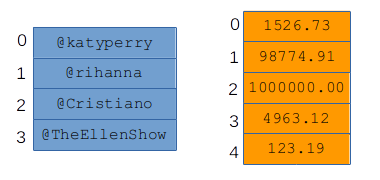
\includegraphics[width=0.6\textwidth]{array.png}
\caption{Two arrays.}
\label{fig:array}
\end{figure}

\index{index@index (pl:~indices)}
\label{arrayIndex}

Worthy of special note are the numbers on the left-hand side. These numbers
are called the \textbf{indices} (singular:~\textbf{index}) of the array.
They exist simply so we have a way to talk about the individual elements. I
could say ``element \#2 of the \texttt{followees} array'' to refer to
\texttt{@Cristiano}.

\index{zero@zero, starting at}
And yes, you noticed that the index numbers start with 0, not 1. Yes, this is
weird. The reason I did that it is because nearly all programming languages
(including Python) number their array elements starting with zero, so you might
as well just start getting used to it now. It's really not hard once you get
past the initial weirdness.

Arrays are the most basic kind of aggregate data there is, and they are the
workhorse of a whole lot of Data Science processing. Sometimes they're called
\textbf{lists}, \textbf{vectors}, or \textbf{sequences}, by the way. (When a
particular concept has lots of different names, you know it's important.)

\index{array!associative}
\index{key-value pair}
\subsection{Associative arrays}
\label{sec:assocArrays}

An \textbf{associative array}, by contrast, has no index numbers. And its
elements are slightly more complicated: instead of just bare values, an
associative array contains \textbf{key-value pairs}.
Figure~\ref{fig:assocArray} shows a couple of examples. The left-hand side of
each picture shows the keys, and the right-hand side the corresponding value.

With an associative array, you don't ask ``what's element \#3?'' like you do
with a regular array. Instead, you ask ``what value is associated with the
\texttt{"Washington"} key?'' And out pops your answer (\texttt{"Redskins"}).

\begin{figure}[ht]
\centering
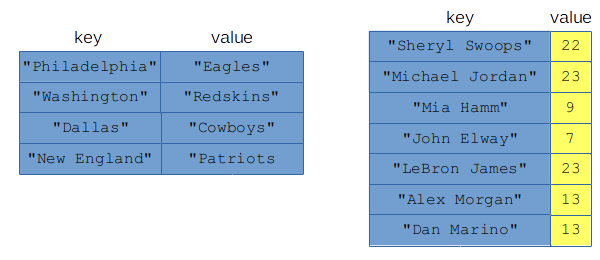
\includegraphics[width=0.9\textwidth]{assocArray.png}
\caption{Two associative arrays.}
\label{fig:assocArray}
\end{figure}

\index{order}
\index{undefined}
\index{mapping (a key to a value)}
All access to the associative array is through the keys: you can change the
value that goes with a key, retrieve the value that goes with a key, or even
retrieve and process \textit{all} the keys and their associated values
sequentially.\footnote{Using something called a ``loop,'' which we'll learn
about a little later in the book.} In that third case, the order in which
you'll receive the key-value pairs is \textbf{undefined} (which means ``not
guaranteed to be consistent'' or ``not necessarily what you'd expect.'') This
underscores the fact that there isn't any reliable ``first'' key-value pair,
or second, or last. They're just kind of all equally ``in there.'' Your mental
model of an associative array should just think of keys that are
\textbf{mapped} to values (we say that \texttt{"Dallas"} is ``mapped'' to
\texttt{"Cowboys"}) without any implied order. (Sure, the
\texttt{"Philadelphia"}/\texttt{"Eagles"} pair is at the top of the picture,
but that's only because I had to put \textit{something} at the top of the
picture, and I chose Philadelphia at random. It doesn't have any meaningful
primacy though.)

\index{homogeneous} Note a couple things about Figure~\ref{fig:assocArray}.
First, the keys in an associative array will almost always (and for us,
\textit{always}) be homogeneous. Similarly, the values will be homogeneous. But
the keys might not be of the same type as the values. In the left picture, both
keys and values are text, but in the right picture, the keys are text and the
values (uniform numbers of famous athletes) are whole numbers. This is
perfectly healthy and good.

\index{uniqueness!of keys in an associative array}
Second, realize that the \textit{keys} in an associative array must be
\textbf{unique} -- this means that there can be no duplicate keys. If we tried
to create a second \texttt{"Alex Morgan"} (oh, if only...) with a different
value, that new value would \textit{replace} Alex's current value, not sit
alongside the first one as an additional key-value pair.

The reverse is not true, however: the \textit{values} of an associative array
may very well not be unique. In the left-hand picture they are, but in the
right-hand picture there are duplicates: both Jordan and LeBron wore \#23 in
their stellar careers, while Hall of Famer quarterback Dan Marino once chose
the same uniform number that Alex wears today. This isn't a problem, because we
always access the information in an associative array \textit{through the
keys}. Asking ``what number did Mia Hamm wear?'' gives us a well-defined
answer. Asking ``which famous athlete wore \#23?'' does not. That's why we
can't ask that second question (and aren't meant to).

\subsection{Tables}

\index{table}

Lastly, we have the table, which in Data Science is positively ubiquitous. In
Figure~\ref{fig:table} we return to the pinterest.com example, with a table of
their most popular users. As you can see, it has more going on that than the
previous two aggregate data types. Still, it's pretty straightforward to wrap
your head around.

\begin{figure}[ht]
\centering
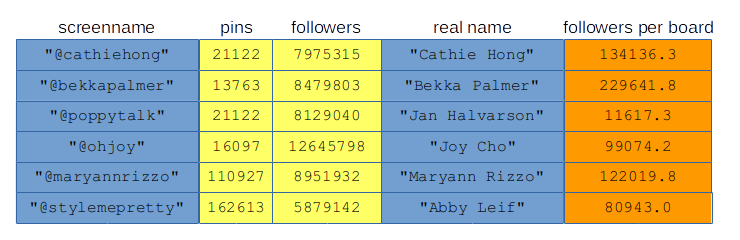
\includegraphics[width=\textwidth]{table.png}
\caption{A table.}
\label{fig:table}
\end{figure}

\index{row (of a table)}
\index{column (of a table)}
Unlike the other two aggregate data types, tables are full-on two-dimensional.
There's (theoretically) no limit to how many \textbf{rows} and how many
\textbf{columns} they can have. By the way, it's important to get those two
terms straight: rows go across, and columns go up and down. (Think of the
columns in the Trinkle Rotunda.) Also, the typical table has many, many more
rows than columns, so they're super tall and skinny, not short and fat.

\index{heterogeneous}
\index{homogeneous}
Although the \textit{rows} of a table are often heterogeneous, each
\textit{column} must be homogeneous. You can see that with a glance at
Figure~\ref{fig:table}. Each column represents a specific type of data -- in
this case, some statistic or piece of information about a Pinterest user.
Clearly all screen names should be of a text type, all ``number of pins or
followers'' should be whole numbers, \textit{etc.} It doesn't make sense
otherwise.

\index{order}
\label{assocArraysUnordered}
As with the other types, the whole dog-gone table -- no matter how many
millions of rows it might have -- is \textit{one} variable with a single name.
Also, just like with associative arrays, there normally isn't any implied
\textit{order} to the rows. Many implementations of these data types (including
Python/Pandas) will actually let you specify ``the first row'' or ``the
$53^{\textrm{rd}}$ row,'' but that always makes me cringe because conceptually,
there isn't any such thing. They're just ``rows'' that are all ``in
there.''

\subsubsection{``Querying'' tables (and other things)}

\index{query}
\label{tablesHaveNoKey}

Now you might be wondering how to actually ``get at'' the individual values of
a table. Unlike arrays, there's no index number. And unlike associative arrays,
there's no key. How then to address, say, the \texttt{@poppytalk} row?

The answer will turn out to be something called a \textbf{query}, which is a
geeky way of saying ``a set of criteria which will match some, but not all, of
the rows and/or columns.'' For instance, we might say ``tell me the pin count
for \texttt{@ohjoy}.'' Or, ``give me all the information for any user who has
more than 100,000 followers per board \textit{and} at least 20,000 pins.''
Those specific requirements will restrict the table to a subset of its rows
and/or columns. We'll learn the syntax for that later. It's a bit tricky but
very powerful.

\index{element}
By the way, it turns out we'll actually be using the concept of a query for
arrays and associative arrays as well. So strictly speaking, a query isn't just
a ``table thing.'' However, they're especially invaluable for tables, since
they're essentially the \textit{only} way to access individual elements.

\section{Aggregate data and memory pictures}

Recall from chapter~\ref{ch:memoryPictures} (p.~\pageref{fig:memoryPicture})
that the right-hand side of our memory pictures bore the label
``\textsf{Aggregate data}.'' You may have anticipated that that's where the
stuff in this chapter will live, and you're right. But there's a catch.
Remember that variable \textit{names} live on the left-hand side, and that's
true even if the variable is of an aggregate type! This turns out to be
crucially important, so I'm going to make a big deal about it.

You must draw your memory pictures (either on a whiteboard, or in your head) in
a very specific way, and that way is illustrated in
Figure~\ref{fig:aggregateMemory}.

\begin{figure}[ht]
\centering
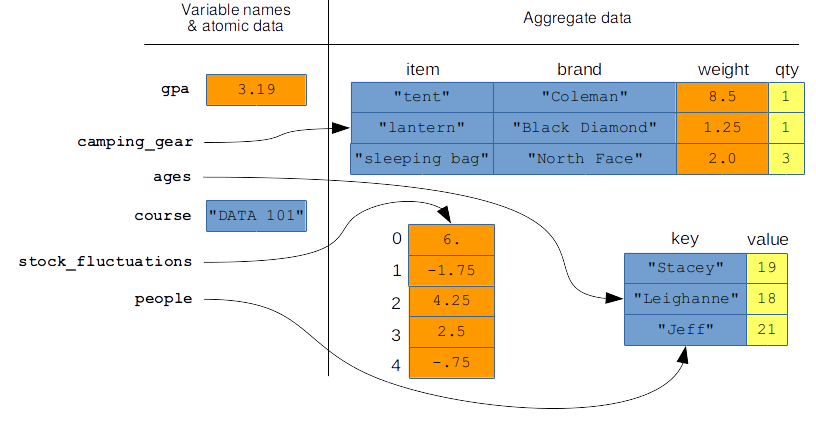
\includegraphics[width=1\textwidth]{aggregateMemory.png}
\caption{Where aggregate data variables -- and their variable names -- live in
memory.}
\label{fig:aggregateMemory}
\end{figure}

Study this picture carefully, and notice several vitally important things.
First, \textit{all} the variable names are on the left-hand side -- whether
aggregate or not. This is always, always true.

\index{pointer}
\index{reference}

Second, the actual array, associative array, and table depicted in this diagram
are on the right-hand side. The variable name on the left ``\textbf{points
to}'' the data in question with a little arrow. The technical name for this
arrow is a \textbf{pointer} or a \textbf{reference}. The rule is simple: each
atomic variable (like \texttt{gpa} or \texttt{course}) contains \textit{the
colored box itself}. Aggregate variables (like the other four) contain
\textit{a pointer to the group of colored boxes.}

Finally, mull over the fact that two \textit{different} variables in this
memory picture are pointing to the same thing! (\texttt{ages} and
\texttt{people}) Believe it or not, this is a normal occurrence. The
consequence is that if Stacey had a birthday, and we increased her age from 19
to 20 in the associative array, \textit{both} \texttt{ages} \textit{and}
\texttt{people} would automatically see the new value. There is only one copy
of that associative array in memory, and both variable names point at it.

It may seem like I'm being pedantic with this left-side-right-side stuff and
all the little arrows. \textbf{I promise you I'm not.} The moment your data
analysis program gets even mildly complicated, you will do the \textit{wrong}
thing and get the \textit{wrong} answers if you don't think of it exactly like
this. Take your time and commit it to memory.


% np.array([]), np.arange(), np.zeros(),
% np.loadtxt("file", dtype=object, delimiter='!!!')
% +, -, *, /
% np.sqrt()
% np.round( , num_decimals)
% np query syntax

% indexing, slices

\chapter{Arrays in Python: NumPy \texttt{ndarray}s}

\index{array!in NumPy}
\index{ndarray@\texttt{ndarray} (NumPy)}
\index{list@\texttt{list}, plain-ol'}
There are several candidates in the Python language for representing the type
of array structure we introduced in chapter~\ref{ch:aggregateData}. One is the
plain-ol' Python \textbf{\texttt{list}}, which you may have used if you've
taken a computer science course in Python. Turns out, \texttt{list}s are going
to be too slow for us once we start dealing with a lot of data, plus there are
a lot of things that it won't do for us automatically that are handy to have.
Another choice is the Pandas \texttt{Series} which we'll actually cover in
chapter~\ref{ch:pythonAssocArrays} -- oddly, that one turns out to do too
\textit{much}, rather than too little, for our purposes here. A happy medium is
the \textbf{\texttt{ndarray}} from the NumPy package\footnote{Most people seem
to pronounce this ``NUM-pie,'' although I've heard ``NUM-pee'' as well. Pick
your poison.}. Before we do that, however, we need to learn what a ``package''
actually is, and how to use one.

\section{Packages}
\index{package}

Back in my day (circa 1990's) when someone wanted to write a computer program,
they wrote the entire thing themselves, line by line. Everything you needed to
do -- from something complex like making a remote network connection to
something simple like computing the average of some numbers -- was up to you to
build. Code sharing over the Internet just wasn't much of a thing.

Today, the reverse is true. When you write a complex data analysis program,
\textit{most} of the code will actually be written by others, if you do it
right. This is because many, many smart people across the globe have written
snippets of code to do all the common (and some not-so-common) things you'll
want to do, and your job is to string them all together. Put another way:
you're given most of the Legos\textsuperscript{\textregistered} -- and even a
bunch of pre-assembled chunks made with dozens of
Legos\textsuperscript{\textregistered} each -- and your job is to construct
your masterpiece out of those building blocks.

\index{package}
\index{importing (a package)}
\index{package}
\index{calling a function@``calling'' a function}
\index{calling a method@``calling'' a method (on a variable)}
In Python, a \textbf{package} is a repository of useful functions and methods
that someone else has written. By \textbf{import}ing a package into your
program, you're making all those useful things available to you. Your own code
can then call those functions/methods whenever you see fit. It's the modular,
organized, and elegant way to do things, in addition to saving a ton of time.

The first package we'll use is called \textbf{NumPy}, which stands for
``Numerical Python.'' To import it, you should include this exact line of code
in the \textit{first} Code cell of your Notebook:

\begin{Verbatim}[fontsize=\small,samepage=true,frame=single,framesep=3mm]
import numpy as np
\end{Verbatim}

Note that it's in all lower-case letters. Once that cell has been executed, you
now have access to all the NumPy ``stuff,'' which is the subject of this
chapter.

\section{The NumPy \texttt{ndarray}}

\index{array}
\index{ndarray@\texttt{ndarray} (NumPy)}
\index{matrix}
The actual data type that the NumPy package provides is called an
\texttt{ndarray}, which stands for ``n-dimensional array.'' If that sounds
heady, it kind of is, although in this course we're only ever going to use a
\textit{one}-dimensional array, which is super simple to understand. In fact,
it looks exactly like the examples in Figure~\ref{fig:array}
(p.~\pageref{fig:array}). ``One-dimensional'' just means that there is a single
index number, and the elements are all in a line.\footnote{A two-dimensional
array is a spreadsheety-looking thing also called a \textbf{matrix}. Each
element has \textit{two} index numbers: a row and a column. A three-dimensional
array is a cube, with three index numbers needed to specify an element.
\textit{Etc.}}

\subsection{Creating \texttt{ndarray}s}

There are many different ways to create an \texttt{ndarray}. We'll learn four
of them.

\subsubsection{Way 1: \texttt{np.array([])}}

\index{array@\texttt{array()} function (NumPy)}
The first is to use the \texttt{array()} function of the NumPy package, and
give it all the values explicitly. Here's the code to reproduce the
Figure~\ref{fig:array} examples:

\begin{Verbatim}[fontsize=\scriptsize,samepage=true,frame=single,framesep=3mm]
followees = np.array(['@katyperry','@rihanna','@Cristiano','@TheEllenShow'])
balances = np.array([1526.73, 98774.91, 1000000, 4963.12, 123.19])
\end{Verbatim}

\index{boxies (square brackets)}
\index{[]@\texttt{[]} (boxies)}
\index{bananas (parentheses)}
\index{()@\texttt{()} (bananas)}
It's simple, but don't miss the syntactical gotcha: \textit{you must include a
pair of boxies inside the bananas.} Why? Reasons.\footnote{For the experienced
reader, what we're actually doing here is creating a plain-ol' Python list
(with the boxies), and then calling the \texttt{array()} function with that
list as an argument.} For now, just memorize that for this function -- and this
function only -- we use ``\texttt{([}\textsl{...stuff...}\texttt{])}'' instead
of ``\texttt{(}\textsl{...stuff...}\texttt{)}'' when we call it.

\index{package}
\index{function}
\index{method}
By the way, the attentive reader might object to me calling \texttt{array()} a
function, instead of a method. Isn't there a word-and-a-dot before it, and
isn't that a ``method thing?'' Shrewd of you to think that, but actually no,
and the reason is that ``\texttt{np}'' isn't the name of a variable, but the
name of a \textit{package}. When we say ``\texttt{np.array()}'' what we're
saying is: ``Python, please call the \texttt{array()} function \textit{from the
\texttt{np} package}.'' The word-and-dot syntax does double-duty.

\index{type@\texttt{type()}}
We can call the \texttt{type()} function, as we did back on
p.~\pageref{typeFunction}, to verify that yes indeed we have created
\texttt{ndarray}s:

\begin{Verbatim}[fontsize=\small,samepage=true,frame=single,framesep=3mm]
print(type(followees))
print(type(balances))
\end{Verbatim}

\begin{Verbatim}[fontsize=\small,samepage=true,frame=leftline,framesep=5mm,framerule=1mm]
numpy.ndarray
numpy.ndarray
\end{Verbatim}

\index{dtype@\texttt{.dtype} (NumPy)}
This is useful, but sometimes we want to know what underlying atomic data type
the array is comprised of. To do that, we attach ``\texttt{.dtype}''
(confusingly, \textit{without} bananas this time) to the end of the variable
name. ``\texttt{.dtype}'' stands for ``data type.'' Here goes:

\begin{Verbatim}[fontsize=\small,samepage=true,frame=single,framesep=3mm]
print(type(followees))
print(type(balances))
\end{Verbatim}

\begin{Verbatim}[fontsize=\small,samepage=true,frame=leftline,framesep=5mm,framerule=1mm]
dtype('<U13')
dtype('float64')
\end{Verbatim}

Whoa, what does \textit{that} stuff mean? It's a bit hard on the eyes, but let
me explain. The underlying data type of \texttt{followees} is (bizarrely)
``\texttt{<U13}'' which in English means ``strings of Unicode
characters\footnote{A ``Unicode character'' is just a fancy way of saying ``a
character, which might not be English.'' NumPy is capable of storing more than
just a-b-c's in its strings; it can store symbols from Greek, Arabic, Chinese,
\textit{etc.} as well.}, each of which is 13 characters long or less.'' (If you
bother to count, you'll discover that the longest string in our
\texttt{followees} array is the last one, \texttt{'@TheEllenShow'}, which is
exactly 13 characters long.) The ``\texttt{float64}'' thing means
``\texttt{float}s, each of which is represented with 64 bits\footnote{A ``bit''
-- which is short for ``binary digit'' -- is the tiniest piece of information a
computer can store: it's a single 0 or 1.} in memory.

You don't need to worry about any of those details. All you need to know is: if
an array's \texttt{dtype} has ``\texttt{<U}'' in it, then it's composed of
strings; and if it has the word ``\texttt{int}'' or ``\texttt{float}'' in it,
it means one of those two old friends from chapter~\ref{ch:atomicData}.

\index{homogeneous}
\index{list@\texttt{list}, plain-ol'}
Incidentally, you'll recall from chapter~\ref{ch:aggregateData} that an array
is \textit{homogeneous}, which means all its elements are of the same type.
NumPy enforces this. If you try to combine them:

\begin{Verbatim}[fontsize=\small,samepage=true,frame=single,framesep=3mm]
weird = np.array([3, 4.9, 8])
strange = np.array([18, 73.0, 'bob', 22.8])
\end{Verbatim}

\index{type@\texttt{type()}}
you'll discover that NumPy converts them to all be of the same type:

\begin{Verbatim}[fontsize=\small,samepage=true,frame=single]
print(weird)
print(weird.dtype)
print(strange)
print(strange.dtype)
\end{Verbatim}

\begin{Verbatim}[fontsize=\small,samepage=true,frame=leftline,framesep=5mm,framerule=1mm]
[ 3.   4.9  8. ]
dtype('<U3')
['18' '73.0' 'bob' '22.8']
dtype('float64')
\end{Verbatim}

See how the \texttt{int}s \texttt{3} and \texttt{8} from the first array were
converted into the \texttt{float}s \texttt{3.}~and \texttt{8.}; meanwhile, all
of the numerical elements of the second array got converted to \texttt{str}s.
(If you think about it, that's the only direction the conversions could go.)

\subsubsection{Way 2: \texttt{np.zeros()}}

\index{increment}
\index{decrement}
\index{counter variable}

It will often be useful to create an array, possibly a large one, with all
elements equal to \textit{zero} initially. Among other scenarios, we often need
to use a bunch of counter variables to, well, count things. Suppose, for
example, that we had a giant array that held the numbers of likes that each
Instagram photo had. When someone likes a photo, that photo's appropriate
element in the array should be \textbf{incremented} (raised in value) by one.
Similarly, if someone unlikes it, then its value in the array should be
\textbf{decremented} by one.

\index{zeros@\texttt{zeros()} function (NumPy)}
An easy way to do this is NumPy's \texttt{zeros()} function:

\begin{Verbatim}[fontsize=\small,samepage=true,frame=single,framesep=3mm]
photo_likes = np.zeros(40000000000)
\end{Verbatim}

(although I'll bet you don't have enough memory on your laptop to actually
store an array this size! Instagram sure has a lot of pics...) When I do this
on my Data Science cluster, I get this:

\begin{Verbatim}[fontsize=\small,samepage=true,frame=single,framesep=3mm]
print(photo_likes)
print(photo_likes.dtype)
\end{Verbatim}

\begin{Verbatim}[fontsize=\small,samepage=true,frame=leftline,framesep=5mm,framerule=1mm]
array([ 0.,  0.,  0., ...,  0.,  0.,  0.])
float64
\end{Verbatim}

Don't miss the ``\texttt{...}'' in the middle of that first line! It means
``there are (potentially) a lot of elements here that we're not showing, for
conciseness.'' Also notice that \texttt{zeroes()} makes an array of
\texttt{float}s, not \texttt{int}s.


\subsubsection{Way 3: \texttt{np.arange()}}

\index{arange@\texttt{arange()} function (NumPy)}
Sometimes we need to create an array with regularly-spaced values, like ``all
the numbers from one to a million'' or ``all even numbers between 20 and 50.''
We can use NumPy's \texttt{arange()} function for this.

\index{type@\texttt{type()}}
Normally we pass this function two arguments, like so:

\begin{Verbatim}[fontsize=\small,samepage=true,frame=single,framesep=3mm]
usa_years = np.arange(1776, 2020)
print(usa_years)
print(usa_years.dtype)
\end{Verbatim}

\begin{Verbatim}[fontsize=\small,samepage=true,frame=leftline,framesep=5mm,framerule=1mm]
[1776 1777 1778 1779 ... 2016 2017 2018 2019]
int64
\end{Verbatim}

If you read that code and output carefully, you should be surprised. We asked
for elements in the range of 1776 to 2020, and we got...1776 through
\textit{2019}. Huh?

\index{OBOE@OBOE (off-by-one error)}
\index{off-by-one error}

Welcome to one of several little Python idiosyncrasies. When you use
\texttt{arange()} you get an array of elements starting with the first
argument, and going up through \textit{but not including} the last number.
There's a reason Python and NumPy decided to do it this way\footnote{Certain
common operations are claimed to be ``simpler'' when you make a range function
work this way. I personally don't buy it: I think it should work in the way you
probably expected (including the second argument). I didn't get a vote,
though.}, but for now it's just another random thing to memorize. If you
forget, you're likely to get an ``OBOE'' -- which stands for ``off-by-one
error'' -- a common programming error where you do \textit{almost} the right
thing but perform one fewer, or one more, operation than you meant to.

Anyways, other than that glitch, you can see that the function did a useful
thing. We can quickly generate regularly-spaced arrays of any range of values
we like. By including a third argument, we can even specify the \textbf{step
size} (the interval between each pair of values):

\begin{Verbatim}[fontsize=\small,samepage=true,frame=single,framesep=3mm]
twentieth_century_decades = np.arange(1900, 2010, 10)
prez_elections = np.arange(1776, 2024, 4)
print(twentieth_century_decades)
print(prez_elections)
\end{Verbatim}

\begin{Verbatim}[fontsize=\small,samepage=true,frame=leftline,framesep=5mm,framerule=1mm]
[1900 1910 1920 1930 1940 1950 1960 1970 1980 1990 2000]
[1776 1780 1784 1788 ... 2008 2012 2016 2020]
\end{Verbatim}

Notice we had to specify 2010 and 2024 as the second argument to these function
calls in order for the arrays to include 2000, and 2020, respectively. This is
the same ``up to but not including the end point'' behavior, but extended to
step sizes of greater than one.



% memory pics


% TODO: np.sqrt()
% TODO: slices

\chapter{Arrays in Python (2 of 2)}
\label{ch:arraysInPython2}

\index{array!in NumPy}
\index{ndarray@\texttt{ndarray} (NumPy)}

Now that we know several options for how to \textit{create} \texttt{ndarrays},
what can we do with them? Many and sundry things.

\section{Getting the array size}

To learn how long an array is (\textit{i.e.}, how many elements) we use the
\texttt{len()} function, kind of like we did for strings. Refer back to
Figure~\ref{fig:arraysInMemory} (p.~\pageref{fig:arraysInMemory}) and consider
this code:

\begin{Verbatim}[fontsize=\footnotesize,samepage=true,frame=single,framesep=3mm]
num_players = len(roster)
sam_len = len(roster[2])
big_number = len(photo_likes)
print("There are {} players on the USWNT.".format(num_players))
print("Sam Mewis has {} characters in her name.".format(sam_len))
print(big_number)
print("We've had {} elections.".format(len(prez_elections)))
\end{Verbatim}

\begin{Verbatim}[fontsize=\footnotesize,samepage=true,frame=single,framesep=3mm]
There are 24 players on the USWNT.
Sam Mewis has 9 characters in her name.
40000000000
We've had 59 elections.
\end{Verbatim}

\label{overloading}
\index{overloading}
\index{return@``returning'' a value}
\index{array!length}
\index{len@\texttt{len()}}
\index{element}
This is an example of Python \textbf{overloading} function names, which just
means that the same name is used for two different functions. When you pass a
string to \texttt{len()}, you get the number of characters; but when you pass
an array to \texttt{len()}, you get the number of elements it has.
(The \texttt{roster} array had way more than 24 \textit{letters} in it, notice
-- but \texttt{len()} returned 24 since that was the number of strings.)

\section{Accessing individual elements}

\subsection{Retrieving an element}

\index{boxies (square brackets)}
\index{[]@\texttt{[]} (boxies)}
\index{element}
To get the value of a specific element from an array, we use ``boxie notation''
with the index number:

\begin{Verbatim}[fontsize=\small,samepage=true,frame=single,framesep=3mm]
print(prez_elections[0])
third_year = usa_years[2]
print("{} was the 3rd year of U.S.A.".format(third_year))
print("The highest-numbered player is {}".format(
    roster[len(roster)-1]))
\end{Verbatim}

\begin{Verbatim}[fontsize=\small,samepage=true,frame=leftline,framesep=5mm,framerule=1mm]
1788.0
1778 was the 3rd year of U.S.A.
The highest-numbered player is Christen Press.
\end{Verbatim}

Remember, indices start at zero (not one) so that's why the first line has a
\texttt{0} in it.

Now examine that last line, which is kind of tricky. Whenever you have boxies,
you have to first evaluate the code \textit{inside} them to get a number. That
number is then the index number Python will look up in the array. In the last
line above, the code \textit{inside} the boxies is:

\quad\quad\quad   ...\texttt{len(roster)-1}...

Breaking it down, we know that \texttt{len(roster)} is 24, which means
\texttt{len(roster)-1} must be 23, and so \texttt{roster[len(roster)-1]} is
\texttt{Christen Press}. It's a common pattern to get the last element of an
array.\footnote{Fun fact: you can also use \textit{negative} indices to mean
``from the end of the array, rather than the beginning.'' So
\texttt{roster[-1]} will also give you \texttt{Christen Press},
\texttt{roster[-2]} is \texttt{Jessica McDonald},
\texttt{roster[-5]} is \texttt{Crystal Dunn}, \textit{etc.} (see
p.~\pageref{rosterNames} for the values). I find this a bit obscure, though, so
I don't normally use this feature. (Negative indices also mean a completely
different thing in the R language, which is another reason I eschew them in
both R and Python.)}

To test your understanding, figure out what the following code will print:

\label{indexTest}
\begin{Verbatim}[fontsize=\small,samepage=true,frame=single,framesep=3mm]
q = 2
r = np.array([45,17,39,99])
s = 1
print(r[q-s+1]+3)
\end{Verbatim}

The answer is at the end of the chapter.

\subsection{Changing an element}

To modify an element of an array, just use the equals sign like we do for
variables:

\index{stooges@Stooges (The Three)}
\index{beavis@Beavis}
\begin{Verbatim}[fontsize=\small,samepage=true,frame=single,framesep=3mm]
stooges = np.array(['Larry','Beavis','Moe'])
print(stooges)
stooges[1] = 'Curly'
print(stooges)
\end{Verbatim}

\begin{Verbatim}[fontsize=\small,samepage=true,frame=leftline,framesep=5mm,framerule=1mm]
['Larry' 'Beavis' 'Moe']
['Larry' 'Curly' 'Moe']
\end{Verbatim}

After all, an individual element like \texttt{stooges[1]} is itself a variable
pretty much like any other.

% Omit: slices

\section{``Vectorized'' arithmetic operators}

Recall our table of Python math operators (Figure~\ref{fig:mathOps} on
p.~\pageref{fig:mathOps}). What do those things do if we use them on aggregate,
instead of atomic data? The answer is: something super cool and useful.

\subsection{Operating on an array and a single value}

Consider the following code:

\label{vectorizedArrayIntExample}
\begin{Verbatim}[fontsize=\small,samepage=true,frame=single,framesep=3mm]
num_likes_today = np.array([6,61,0,0,14])
num_likes_tomorrow = num_likes_today + 3
print(num_likes_tomorrow)
\end{Verbatim}

\begin{Verbatim}[fontsize=\small,samepage=true,frame=leftline,framesep=5mm,framerule=1mm]
[ 9 64 3 3 17 ]
\end{Verbatim}

See what happened? ``Adding 3'' to the \textit{array} means adding 3 \textit{to
each element}. All in one compact line of code, we can do five -- or even five
billion -- operations. This works for all the other Figure~\ref{fig:mathOps}
operators as well.

\index{vectorized@``vectorized'' operation}

For somewhat geeky reasons, this sort of thing is called a \textbf{vectorized}
operation. All you need to know is that this means \textbf{fast}. And that's
``fast'' in two different ways: fast to write the code (since instead of using
a \textbf{loop}, which we'll cover in \ref{ch:loops}, you just write a single
statement with \texttt{+} and \texttt{=} signs), and more importantly, fast to
\textit{execute}. For more geeky reasons, the above code will run lightning
fast even if \texttt{num\_likes\_today} had five hundred million elements
instead of just five. As you'll learn if you ever try it, a Python loop is much
slower.\footnote{I just ran that comparison on my laptop, and here are the
results. Using the plain-ol' ``\texttt{+}'' vectorized operator, my machine
added the number 3 to an array with five hundred million elements in just 1.51
seconds. A loop, by contrast, took 2.8 \textit{minutes} to do the same thing.}

Don't get me wrong: there are times we'll have to use a loop because we have no
choice. But the general rule with Python is: if you can figure out how to
perform a calculation without using a loop, always do it!


\subsection{Operating on two arrays}

\index{vectorized@``vectorized'' operation}

Possibly even cooler, we can even ``\texttt{+}'' (or ``\texttt{-}'', or
``\texttt{*}'', or...) two entire \textit{arrays} together. Example:

\label{vectorizedArrayArrayExample}
\begin{Verbatim}[fontsize=\small,samepage=true,frame=single,framesep=3mm]
salaries = np.array([38000, 102000, 55750, 29500, 250000])
raises = np.array([1000, 4000, 2000, 1000, 2000])
salaries = salaries + raises
print(salaries)
\end{Verbatim}

This code produces:

\begin{Verbatim}[fontsize=\small,samepage=true,frame=leftline,framesep=5mm,framerule=1mm]
[ 39000 106000 57750 30500 252000]
\end{Verbatim}

Can you see why? ``Adding'' the two arrays together performed addition
\textit{element-by-element}. The result is a new array with $38000+1000$ as the
first element, $102000+4000$ as the second, \textit{etc.} This, too, is a
lightning-fast, vectorized operation, and it too works with all the other math
operators.

Just to re-emphasize one point before we go on. In the example back on
p.~\pageref{vectorizedArrayIntExample}, we assigned the result of the operation
to a new variable, \texttt{num\_likes\_tomorrow}. This means that
\texttt{num\_likes\_today} itself was \textit{unchanged} by the code. In
contrast, in the example we just did, we assigned the result of the operation
back into an \textit{existing} variable (\texttt{salaries}). So
\texttt{salaries} has itself been updated as a result of that code.

% TODO: could include memory picture to this effect.


\section{Copying -- and \textit{not} copying -- arrays}

\label{copyingNotCopyingArrays}
\index{copying@copying (arrays)}
Now, a surprise for the unwary. Suppose I write this code:

\label{code:refNotCopy}
\begin{Verbatim}[fontsize=\small,samepage=true,frame=single,framesep=3mm]
stooges = np.array(['Larry','Beavis','Moe'])
funny_people = stooges
stooges[1] = 'Curly'
print("The stooges are: {}.".format(stooges))
print("The funny people are: {}.".format(funny_people))
\end{Verbatim}

Take a moment and predict what you think the output will be. Then, read it and
(possibly) weep:

\begin{Verbatim}[fontsize=\small,samepage=true,frame=leftline,framesep=5mm,framerule=1mm]
The stooges are: ['Larry' 'Curly' 'Moe'].
The funny people are: ['Larry' 'Curly' 'Moe'].
\end{Verbatim}

Note carefully: \textit{no \texttt{Beavis}}.

\begin{figure}[ht]
\centering
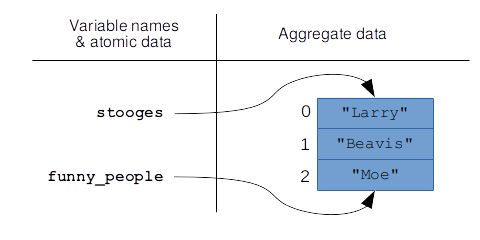
\includegraphics[width=0.49\textwidth]{refNotCopy.png}
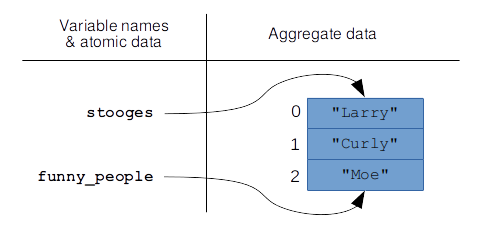
\includegraphics[width=0.49\textwidth]{refNotCopy2.png}
\caption{The code on p.~\pageref{code:refNotCopy} immediately before (left
side) and after (right side) the line ``\texttt{stooges[1] = \textquotesingle
Curly\textquotesingle}'' is reached.}
\label{fig:refNotCopy}
\end{figure}

\index{memory!picture}

Now the question is why. To understand this (and virtually any other tricky
programming problem) you have to return once again to the memory picture.
Figure~\ref{fig:refNotCopy} shows the situation immediately before, and after,
the line ``\texttt{stooges[1] = \textquotesingle Curly\textquotesingle}''
executes. Crucially, \textit{there is only one array} in memory. Both variables
-- \texttt{stooges} and \texttt{funny\_people} -- are pointing at it.

You see, if \texttt{y} contains \textit{aggregate} (instead of atomic) data,
the line ``\texttt{x = y}'' does not perform a copy operation. Instead, it just
points the \texttt{x} variable name to the same place \texttt{y} is pointing
to.

Once you grasp this, it's easy to see why \texttt{"Beavis"} completely
disappeared. There's only one array at all, so changing \texttt{stooges} has
the side effect of implicitly changing \texttt{funny\_people} as well.

\subsection{Actually copying}

The ``point the variable to the same thing, but don't do a copy'' behavior is
the default, because such copy operations are expensive (in terms of memory
usage and time to execute). They're normally not what you want anyway.
Sometimes, however, you \textit{do} want to produce an entire separate copy of
an array, so you can modify the copy yet preserve the original. To do so, you
use the \texttt{.copy()} method:

\begin{Verbatim}[fontsize=\footnotesize,samepage=true,frame=single,framesep=3mm]
orig_beatles = np.array(['John', 'Paul', 'George', 'Pete'])
beatles = orig_beatles.copy()
beatles[3] = 'Ringo'
print("The Beatles were originally {}.".format(orig_beatles))
print("But the ones we all know were {}.".format(beatles))
\end{Verbatim}

Look carefully at that second line: it makes all the difference. Instead of
making the new variable \texttt{beatles} point to the same array in memory that
\texttt{orig\_beatles} did, we explicitly copied the array and made
\texttt{beatles} point to that new copy. The final memory picture is thus as
per Figure~\ref{fig:copyNotRef}, and the output is of course:

\begin{Verbatim}[fontsize=\footnotesize,samepage=true,frame=leftline,framesep=5mm,framerule=1mm]
The Beatles were originally ['John' 'Paul' 'George' 'Pete'].
But the ones we all know were ['John' 'Paul' 'George' 'Ringo'].
\end{Verbatim}

\begin{figure}[ht]
\centering
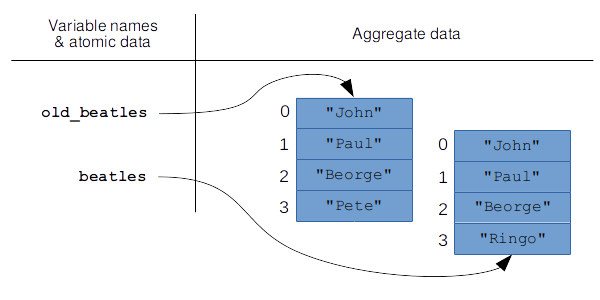
\includegraphics[width=0.9\textwidth]{copyNotRef.png}
\caption{The memory picture after calling the \texttt{.copy()} method, instead
of simply assigning to a new variable.}
\label{fig:copyNotRef}
\end{figure}


\section{Sorting arrays}

\label{sortingArrays}
\index{sorting@sorting (arrays)}
\index{int@\texttt{int}}
\index{float@\texttt{float}}
\index{str@\texttt{str}}
A common operation in Data Science is to \textbf{sort} an array, either
numerically (if the array contains \texttt{int}s or \texttt{float}s) or
alphabetically (if it contains strings). There are two ways to do this, which
turn out to differ in exactly the same was as the operations in the previous
section.

\index{on@``on''}
\index{sort@\texttt{.sort()}}
\index{in place@``in place''}
\index{calling a method@``calling'' a method (on a variable)}
One way is to call the \texttt{.sort()} method directly \textbf{on} an array.
This sorts the array \textbf{in place}, which means that the actual data in
memory is rearranged right then and there. As an important side effect, any
\textit{other} variable that points to the same array will \textit{also} be
sorted.

Here's an example:

\begin{Verbatim}[fontsize=\small,samepage=true,frame=single,framesep=3mm]
gpas = np.array([2.86, 3.99, 3.12, 1.17])
gpas2 = gpas.copy()
gpas3 = gpas
gpas.sort()
print("gpas has: {}".format(gpas))
print("gpas2 has: {}".format(gpas2))
print("gpas3 has: {}".format(gpas3))
\end{Verbatim}

\begin{Verbatim}[fontsize=\small,samepage=true,frame=leftline,framesep=5mm,framerule=1mm]
gpas has: [1.17 2.86 3.12 3.99]
gpas2 has: [2.86 3.99 3.12 1.17]
gpas3 has: [1.17 2.86 3.12 3.99]
\end{Verbatim}

Do you see why that output was produced? It's because the memory picture after
the ``\texttt{gpas.sort()}'' line looks like Figure~\ref{fig:dotSortArray}. The
\texttt{gpas} variable really \textit{is} the \texttt{gpas3} variable, so when
one is sorted, the other automatically is. They're both distinct from
\texttt{gpas2}, though.

\begin{figure}[ht]
\centering
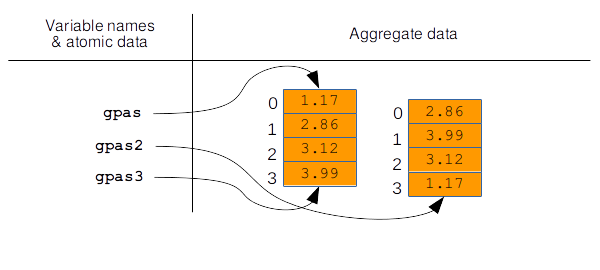
\includegraphics[width=0.9\textwidth]{dotSortArray.png}
\caption{The state of affairs after \texttt{.sort()}ing the \texttt{gpas} array in place.}
\label{fig:dotSortArray}
\end{figure}

\index{sorting@sorting (arrays)}
\index{sort@\texttt{np.sort()} (NumPy)}
\index{calling a function@``calling'' a function}
\index{passing an argument@``passing'' an argument}
The second option is to call the \texttt{np.sort()} function and pass an array
as an object. Like many Python functions, including the ones in the next
section, \texttt{np.sort()} \textit{returns a modified copy} of its argument
rather than changing it in place. To illustrate:

\index{Ravens, Baltimore}
\index{Patriots, New England}
\index{Broncos, Denver}
\index{Steelers, Pittsburgh}
\begin{Verbatim}[fontsize=\small,samepage=true,frame=single,framesep=3mm]
nfl_teams = np.array(["Ravens", "Patriots", "Broncos",
    "Chargers", "Steelers"])
sorted_teams = np.sort(nfl_teams)
print(nfl_teams)
print(sorted_teams)
\end{Verbatim}

\begin{Verbatim}[fontsize=\small,samepage=true,frame=leftline,framesep=5mm,framerule=1mm]
['Ravens' 'Patriots' 'Broncos' 'Chargers' 'Steelers']
['Broncos' 'Chargers' 'Patriots' 'Ravens' 'Steelers']
\end{Verbatim}

\index{return value}
Observe that the \texttt{nfl\_teams} variable, even though we passed it to
\texttt{np.sort()}, was not \textit{itself} sorted. The \texttt{sorted\_teams}
variable, on the other hand, \textit{is} alphabetically sorted, because we
assigned the return value from \texttt{np.sort()} to it. Again, the memory
picture is shown in Figure~\ref{fig:npSortArray}.

\index{on@``on''}
\begin{figure}[ht]
\centering
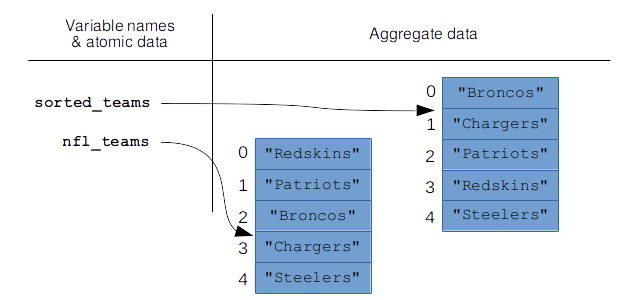
\includegraphics[width=0.9\textwidth]{npSortArray.pdf}
\medskip
\caption{Calling the \texttt{np.sort()} function (as opposed to calling the
\texttt{.sort()} method \textbf{on} the array) returns a sorted copy.}
\label{fig:npSortArray}
\end{figure}

To be clear, either one of these techniques can be used on \textit{any}
\texttt{ndarray}: whole numbers, real numbers, or text. I just chose to do real
numbers in the first example and text in the second. The difference between the
two is merely in what is affected: in one, the actual array in memory is
modified, and in the other, a modified copy is returned.

\section{More exotic array modifications}

\index{in place@``in place''}
There are lots of additional things you can do to an array to either modify its
structure or rearrange its contents. Here's a few. \textbf{Important: all of
the functions in this section return a modified copy of the array you pass to
it. They do \textit{not} change the array in place.}

\begin{itemize}
\itemsep.1em
\index{concatenating!arrays}
\index{append@\texttt{append()} (NumPy)}
\index{insert@\texttt{insert()} (NumPy)}
\index{delete@\texttt{delete()} (NumPy)}
\index{flip@\texttt{flip()} (NumPy)}
\index{reversing (an array)}
\item \texttt{np.append()} can be used to add a single element to the end of an
array, or to add an entire second array of elements to it. (In the latter case,
this is really \textbf{concatenation} of arrays.)
\item \texttt{np.insert()} is like the first form of \texttt{np.append()},
except it inserts in the middle (or the beginning).
\item \texttt{np.delete()} will remove an element of an array \textit{by
position}. In other words, you tell it which \textit{index number} to remove,
not which element.
\item \texttt{np.flip()} reverses the order of elements in an array.
\end{itemize}

These functions are all summarized in Figure~\ref{fig:handyNumPy}.

Remember that when you're calling a function like this -- which returns a
modified copy -- it is perfectly acceptable to store the return value
\textit{in the same variable} that you passed it. This is common if you don't
actually want to keep around the original:

\begin{Verbatim}[fontsize=\small,samepage=true,frame=single,framesep=3mm]
ice_cream_flavors = np.flip(ice_cream_flavors)
\end{Verbatim}

In this pattern, the net effect \textit{is} effectively to modify the array in
place, since you're making a reversed copy, and then assigning that reversed
copy to the same variable.

Anyway, here's some example code to illustrate the functions in this section:

\begin{Verbatim}[fontsize=\small,samepage=true,frame=single,framesep=3mm]
clowns = np.array(["Bozo", "Krusty"])
more_clowns = np.array(["Pennywise", "Skelton"])
more_clowns = np.insert(more_clowns, 1, "Happy Slappy")
all_clowns = np.append(clowns, more_clowns)
all_clowns = np.append(all_clowns, "Ronald McDonald")
all_clowns = np.flip(all_clowns)
all_clowns = np.delete(all_clowns, 2)
print("clowns is: {}".format(clowns))
print("more_clowns is: {}".format(more_clowns))
print("all_clowns is: {}".format(all_clowns))
\end{Verbatim}

\begin{Verbatim}[fontsize=\footnotesize,samepage=true,frame=leftline,framesep=5mm,framerule=1mm]
clowns is: ['Bozo' 'Krusty']
more_clowns is: ['Pennywise' 'Happy Slappy' 'Skelton']
all_clowns is: ['Ronald' 'Skelton' 'Pennywise' 'Krusty' 'Bozo']
\end{Verbatim}

% TODO: memory picture of the clowns

An \textit{excellent} exercise to help cement your understanding of the ideas
in this chapter would be to go through the above ``clowns'' code line by line,
drawing the memory picture as you go, and then confirm that your output matches
the actual output.

\smallskip

Yes, an \textit{excellent} exercise indeed!

\bigskip

\section[Characters within a string]{Postlude: characters within a string}

\index{string}
\index{str@\texttt{str}}

These two chapters have dealt with arrays, but let me say a word at this point
about \textit{strings}, and how they can be made to act like arrays in some
respects.

I mentioned earlier in the book (p.~\pageref{tiptoe}) that strings, though
normally treated as atomic, sometimes tiptoe up to the ``atomic/aggregate''
line and even cross it. In other words, we will occasionally look at individual
parts of a string variable rather than the entire thing as one lump.

\index{boxies (square brackets)}
\index{[]@\texttt{[]} (boxies)}

The way we access individual characters within a string is actually the same
boxie notation we use for arrays. So this code:

\vspace{-.15in}
\begin{Verbatim}[fontsize=\small,samepage=true,frame=single,framesep=3mm]
antihero = "Light Yagami"
print(antihero[0])
letter1 = antihero[6]
letter2 = antihero[7]
print("{}{}{}".format(letter1,letter2,letter1))
\end{Verbatim}
\vspace{-.1in}

will give this output:

\vspace{-.15in}
\begin{Verbatim}[fontsize=\small,samepage=true,frame=leftline,framesep=5mm,framerule=1mm]
L
YaY
\end{Verbatim}
\vspace{-.1in}

\index{zero@zero, starting at}

As you can see, string indexes use the same starting-at-zero nonsense that
arrays do. Hey, at least it's consistent.

\bigskip

\index{overloading}
This is actually another example of overloading. Just as the \texttt{len()}
function means two different things, depending on whether you're asking for the
length of an array or the length of a string (recall p.~\pageref{overloading}),
so the boxie notation means two different things. You're either getting a
specific element out of an array, or a specific character out of a string.

\section{Summary}

The table in Figure~\ref{fig:handyNumPy} gives the promised summary of
the array functions, methods, and operators in this chapter.

\setlength\extrarowheight{5pt}

\begin{figure}[ht]
\centering
\footnotesize
\begin{tabular}{c|p{3.1in}}
Function & Description \\
\hline

\texttt{len(}\textsl{arr}\texttt{)} & Get the number of elements in the array \textsl{arr}. \\

\textsl{arr}\texttt{[17]} & Get a specific element's value from the array \textsl{arr}. \\

\textsl{arr}\texttt{[8] =} (\textsl{something}) & Set a specific element of the array \textsl{arr}. \\

\textsl{arr} \texttt{+ 91} & Add a value to each element of \textsl{arr},
yielding a new array. (Also works with \texttt{-}, \texttt{*}, \texttt{/},
\textit{etc.}) \\

\textsl{arr1} \texttt{+} \textsl{arr2} & Add each pair of values in two arrays,
yielding a new array. (Also works with \texttt{-}, \texttt{*}, \texttt{/},
\textit{etc.}) \\

\textsl{arr1} = \textsl{arr2} & Make \textsl{arr1} point to the same data that
\textsl{arr2} points to. (\textit{Not} a copy!)\\

\textsl{arr1} = \textsl{arr2}\texttt{.copy()} & Make \textsl{arr1} point to a
new, independent copy of \textsl{arr2}. \\

\textsl{arr}\texttt{.sort()} & Sort the array \textsl{arr} \textbf{in place}. (Numerical or
alphabetical, depending on the \texttt{.dtype}.) \\

\texttt{np.sort(}\textsl{arr}) & Return a new array with the sorted elements
of \textsl{arr}. (Numerical or alphabetical, depending on the \texttt{.dtype}.)
\\

\texttt{np.append(}\textsl{arr}, \textsl{elem}\texttt{)} &
    Return a new array with \textsl{elem} tacked on to the end. \\

\texttt{np.append(}\textsl{arr1}, \textsl{arr2}\texttt{)} &
    Return a new array with the two arrays \textsl{arr1} and \textsl{arr2} concatenated. \\

\texttt{np.insert(}\textsl{arr}, \textsl{ind}, \textsl{val}\texttt{)} &
    Return a new array with the new value \textsl{val} inserted into position \textsl{ind} of \textsl{arr}. \\

\texttt{np.delete(}\textsl{arr}, \textsl{ind}\texttt{)} &
    Return a new array with the element at index \textsl{ind} removed from \textsl{arr}. \\

\texttt{np.flip(}\textsl{arr}\texttt{)} &
    Return a new array with \textsl{arr} in reverse order. \\
\end{tabular}
\bigskip
\caption{Handy NumPy functions, methods, and operators.}
\label{fig:handyNumPy}
\end{figure}

\vfill
\subsubsection{The answer}

\index{42 (Life, Universe, Everything)}
Oh, and the answer to the puzzle on p.~\pageref{indexTest} -- and also the
answer to Life, the Universe, and Everything, as it turns out -- is 42.



\chapter{Interpreting Data}

Let's take an intermission from the nitty-gritty Python stuff and talk about
how to properly \textit{interpret} the data we're working with; specifically,
how to draw correct conclusions from what we've collected.

\section{Independent and dependent variables}

\index{variable!dependent}
\index{variable!independent}
\index{independent variable (i.v.)}
\index{dependent variable (d.v.)}
\index{cause}
\index{causal}
\index{hiccup}
\index{greenhouse gas}
\index{smoking}
\index{lung cancer}
\index{global warming}

You've undoubtedly seen countless studies that claim to reveal important truths
about the world, such as that smoking can cause lung cancer, greenhouse gas
emissions can cause higher global temperatures, or orgasms can cure hiccups.
Much of the time, scientists try to find a \textbf{causal} factor that links
one variable to another: they suspect that the value of a variable $A$ (often
called the \textbf{independent variable}, or ``\textbf{i.v.}''~for short) is a
\textit{reason}, or \textbf{cause}, of a certain value in another variable $B$
(the \textbf{dependent variable}, or ``\textbf{d.v.}'').

Just to avoid misunderstandings, when we claim that $A$ \textbf{causes} $B$, we
don't normally mean that it \textit{exclusively} causes it, or even that it
\textit{reliably} causes it. There are lots of contributing factors to lung
cancer besides smoking, after all; and tons of smokers never develop cancer. We
simply mean that $A$ is a contributing factor to $B$, and that the value of the
$A$ variable exerts some, but not total, influence over the value of the $B$
variable.

\index{variable}
\index{objects (of a study)}

Importantly, we're using the word \textbf{variable} here in a different, but
related way than we used it in chapters~\ref{ch:atomicData},
\ref{ch:arraysInPython1}, and \ref{ch:arraysInPython2}. As we did in
chapter~\ref{ch:scalesOfMeasure} (see p.~\pageref{variableDifferent} footnote),
we use ``variable'' here to mean a specific aspect of the \textbf{objects of a
study} that can differ, or ``vary.'' The objects in our study (often people,
but sometimes companies, organizations, environments, nations, \textit{etc.})
\textit{each} have a value for the variable. Thus if you think of a
``per-capita income'' variable, you might think of an entire \textit{array} of
floats, each of which represented the average income-per-resident of a single
nation.

\index{scales of measure}
\index{categorical variable}

The variables in question can be from any of the scales of measure from
chapter~\ref{ch:scalesOfMeasure}. Take the smoking example, with patients as
the object of study. We might say that independent variable $A$ is categorical,
with values \texttt{SMOKER} and \texttt{NON-SMOKER}. The dependent variable $B$
is also categorical: \texttt{CANCER} and \texttt{NO-CANCER}. The key question
is: do people with $A=\texttt{SMOKER}$ also have $B=\texttt{CANCER}$
\textit{more often} (a higher percentage of the time) than people with
$A=\texttt{NON-SMOKER}$ do?

\index{ratio variable}
\index{interval variable}

In the greenhouse gas emissions example, our objects of study might be
\textit{years}. Our variables are both numeric, with $A$ (a measure of yearly
greenhouse gas emissions, measured in gigatonnes $\textrm{CO}_2$) on the ratio
scale, and $B$ (average worldwide temperature increase/decrease) on an interval
scale. Here, the question would be: do years in which $A$ is relatively high
typically also have $B$ relatively high? Put another way: do years in which
earthlings have released more gas into the atmosphere tend to correspond with
years in which the global temperature increased?

And of course, we might have one categorical variable and one numeric. Perhaps
our objects of study are American adults, and while our categorical $A$
variable has values \texttt{DEMOCRAT}, \texttt{REPUBLICAN}, \texttt{OTHER}, and
\texttt{INDEPENDENT}, our numerical $B$ is yearly income. Our question would
be: do adherents of one political party tend to be more wealthy than those of
another?

Or, flipping sides, the independent variable $A$ could be numeric while the
dependent variable $B$ is categorical. Our objects of study might be high
school seniors applying to UMW. Let $A$ be the number of different colleges a
student applied to, and $B$ a categorical variable with values
\texttt{ADMITTED-TO-UMW} and \texttt{NOT-ADMITTED-TO-UMW}. The question of
interest is here is: do students who apply to more colleges tend to get in to
UMW more often?

\section{Association and causality}

\label{association}

All of the above questions can be answered with data. In future chapters, we'll
learn the exact Python commands to ask them, and how to interpret the answers.

\index{association}
\index{correlation}
\index{dependent}

For now, I merely want to draw your attention to the fact that these are all
questions of \textbf{association}, not causation. An association between
variables merely means that they are \textbf{correlated} in some way
statistically.\footnote{Another way to put this is to say that the variables
are \textbf{dependent} on each other, although this is confusing because we're
already using the word ``dependent'' to refer to one of the variables.} If
$A=\texttt{SMOKER}$ goes with $B=\texttt{CANCER}$ more often than
$A=\texttt{NON-SMOKER}$ does, then there \textit{is} an association between the
two, period. If yearly income $B$ is on average higher for
$A=\texttt{REPUBLICAN}$ than for $A=\texttt{DEMOCRAT}$, then there \textit{is}
an association between the two, period.

\label{howMuchMore}

(By the way, a key nuance will turn out to be: \textit{how much} more often
does $A=\texttt{SMOKER}$ need to go with $B=\texttt{CANCER}$ in order for us to
be confident that there is a true association? Or \textit{how much} more
wealthy do the $A=\texttt{REPUBLICAN}$s need to be on average for us to have
confidence we've identified a real link to political party? That one's a little
tricky, and we'll postpone addressing it for now.)

\index{causality}
\label{pythonAssociation}

So anyway, the question of association turns out to be pretty straightforward
to answer. Python will simply tell us if variables are associated or not. More
difficult, however, is determining \textbf{causality}
(a.k.a.~\textbf{causation}). Does a person's political affiliation influence
how much wealth they have? Or is it the other way around: does a person's
wealth cause them to vote a certain way? Or is it neither of these, with some
third factor (perhaps values, or life philosophy) helping determine
\textit{both} variables?

\index{$\rightarrow$@$\rightarrow$ (causality)}

If the first of these three is the case, we would write ``$A \rightarrow B$,''
pronounced ``$A$ causes $B$''. If the second, we'd write, ``$B \rightarrow
A$,'' and for the third, we'd write ``$C \rightarrow A, B$'' for some other
(possibly yet to be determined) variable $C$. Determining which (if any) of
these is true calls for some careful thinking, intuition, and additional kinds
of statistical tests.

In fact, just to blow your mind, Figure~\ref{fig:causalityTypes} gives a
partial list of the various types of causation that \textit{could} be the true
explanation, once we find out that $A$ and $B$ have an association. As you can
see, there are a lot of ways to go wrong. Only \textit{one} of the
possibilities is that ``$A$ actually causes $B$,'' which is what we suspected
in the first place. The others are all ways of producing that same association
we picked up in the data.

\begin{figure}[ht]
\small
\centering
\begin{tabular}{|c|c|p{3.3in}|}
\hline
Symbology & Name & Example \\
\hline
\multirow[c]{2}{*}{$A \rightarrow B$} & \multirow[c]{2}{*}{causation} & Regular
exercise does indeed normally lead to a lower resting heart rate. \\
\hline
\multirow[c]{2}{*}{$B \rightarrow A$} & \multirow[c]{2}{*}{reverse causation} & Smoking doesn't cause depression;
depression causes smoking. \\
\hline
\multirow[c]{2}{*}{$C \rightarrow A, B$} & \multirow[c]{2}{*}{\makecell{external causation \\ (confounding
factor)}} & Ice cream sales don't cause shark attacks; high temperatures boost both ice
cream sales and ocean swimming. \\
\hline
\multirow[c]{2}{*}{$A \rightarrow B$ \& $B \rightarrow C$} &
\multirow[c]{2}{*}{multiple causation }& A liberal arts
education does improve critical thinking skills, but lots of other things do
too. \\
\hline
\multirow[c]{2.5}{*}{$A,C \rightarrow B$} & \multirow[c]{2.5}{*}{joint causation} &
Just being tall doesn't necessarily make you a good basketball player, but if
your height is accompanied by another factor as well (athleticism), then you
will be. \\
\hline
\multirow[c]{2.5}{*}{$A \rightarrow C \rightarrow B$} &
\multirow[c]{2.5}{*}{indirect causation} & People who use antiperspirant tend to
get more dates, but it's not because of the antiperspirant \textit{per se};
it's because they don't have an unpleasant odor. \\
\hline
\multirow[c]{3}{*}{$A \not\rightarrow B$} & \multirow[c]{3}{*}{spurious
association} & Although for many years the outcome of the Washington Redskins
game immediately preceding a Presidential election predicted the election's
outcome, that was by coincidence. \\
\hline
\end{tabular}
\medskip
\caption{Various types of causality that could be the underlying reason why an
association between $A$ and $B$ exists.}
\label{fig:causalityTypes}
\normalsize
\end{figure}

\section{Confounding factors}

\index{confounding factor}
\index{external causation}
\index{variable!confounding}

Let me speak to two of the items in the Figure~\ref{fig:causalityTypes} table
in particular. The third one on the list, \textbf{external causation}, is a
case where a third variable (call it $C$) comes into play. We refer to this as
a \textbf{confounding factor} (or \textbf{confounding variable}) because it
``confounds'' us: causes us to interpret the meaning behind the data in an
incorrect way. The example in the table is a famous and funny one: clearly
sharks don't react to Ben \& Jerry's daily net profits, and people (probably)
don't run out and buy ice cream to cope with their anxiety about shark attacks.
Neither $A \rightarrow B$ nor $B \rightarrow A$, but a third variable -- hot
days -- influence both of them.

\index{causal diagram}
\index{barbecue}
\index{cancer}
\label{barbecue}

Now of course it's not always this obvious. Here's an example I ran across
recently. A magazine article reported on a new health scare: scientists have
discovered that \textit{eating barbecue can increase your risk of cancer.}
Pictorially, this claim is illustrated in the \textbf{causal diagram} in
Figure~\ref{fig:causalDiagram}, which shows our i.v.~and our d.v.~; the arrow
means exactly what it meant earlier.

\begin{figure}[ht]
\centering
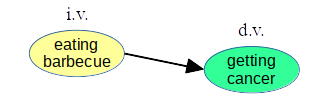
\includegraphics[width=0.6\textwidth]{causalDiagram.png}
\caption{A hypothesis as to causality: eating barbecued foods increases one's
risk for certain types of cancer.}
\label{fig:causalDiagram}
\end{figure}

Unlike sharks and ice cream, this one seems plausible. And I'm not claiming to
have read enough about their study to tell whether the researchers' claim is
bogus. But I couldn't help thinking that there are a great many possibly
confounding factors that could be blurring the results. For one, choosing to
eat barbecue a lot is probably often associated with a less healthy, higher-fat
diet in general (I can speak from experience on that). If that's true, and if
high-fat diets -- whether featuring lots of barbecue or not -- are associated
with these same poor health outcomes, then we'd have the picture on the
left-side of Figure~\ref{fig:causalDiagram23}. The red bubble represents the
confounding factor, which is influencing both i.v.~and d.v. If this picture
were the correct one of the underlying phenomenon, then the correlation we
thought were picking up between barbecue and cancer was actually due to fat
content.

\begin{figure}[ht]
\centering
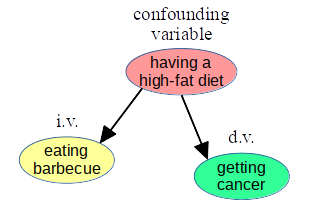
\includegraphics[width=0.4\textwidth]{causalDiagram2.png}
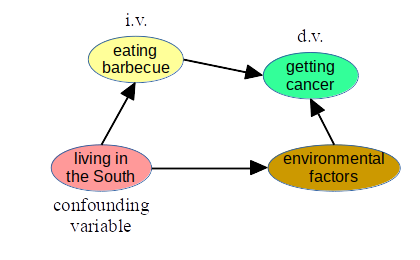
\includegraphics[width=0.5\textwidth]{causalDiagram3.png}
\caption{Other hypotheses as to causality, each resulting in the same
associations in the data, yet involving confounding factors.}
\label{fig:causalDiagram23}
\end{figure}

Another example is the right-hand side of Figure~\ref{fig:causalDiagram23}.
Perhaps barbecue is more popular culturally in some areas of the country (say,
the South, where I certainly see it eaten a lot), and perhaps those areas have
other environmental factors that can lead to cancer. In this case, the
``South'' confounder indirectly affects the d.v.~(via another variable,
representing the environment) but it still affects it.

It's not hard to think of others. These were just the first two that came to
mind. The point is that it's really hard to be sure you've thought of all of
them!


\subsection{Paranoia and overparanoia}

All this should lead you to be somewhat paranoid, but not
\textit{over}paranoid. Confounding variables can definitely lead us to make
mistakes in our reasoning, but perhaps they're not \textit{quite} as common as
you think. Understand that a confounding factor is \textit{not} simply any
other factor that affects the dependent variable. Instead, for a variable to be
confounding \textbf{it must affect both the independent \textit{and} the
dependent variable.}

Let me illustrate with an example. I suspect that on average, men are taller
than women. And I further suspect that there's causality here, and that it goes
from $A$ (sex) to $B$ (height), not the other way around. (Clearly people don't
spontaneously ``turn male'' because they reach a certain height.) So my
thinking on the subject is summed up in Figure~\ref{fig:sexHeight}.

\begin{figure}[ht]
\centering
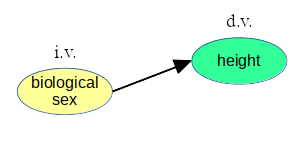
\includegraphics[width=0.6\textwidth]{sexHeight.png}
\caption{Stephen's hypothesis: a person's biological sex (male or female) plays
a causal role in determining their height.}
\label{fig:sexHeight}
\end{figure}

Now let me show you what I mean by ``overparanoia.'' What if someone said,
``but wait, Stephen, not so fast! You've got potential confounding variables
out the wazoo! Why, surely heredity plays some role in a person's height --
tall parents are more likely to have tall offspring, just due to genetics. And
nutrition, too, is a factor: it's been demonstrated that impoverished
communities suffering from malnutrition will have children with stunted growth.
And heck, if you're born at a high elevation (like Nepal), there's less
gravitational pull dragging your body down to earth, so it stands to reason
that you'll probably grow taller. And on and on!'' Figure~\ref{fig:sexHeight2}
depicts this (supposed) scientific nightmare.

\begin{figure}[ht]
\centering
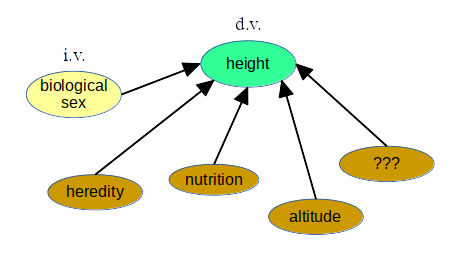
\includegraphics[width=0.7\textwidth]{sexHeight2.png}
\caption{Oh geez -- confounding variables galore? \textbf{\textit{No!}}}
\label{fig:sexHeight2}
\end{figure}

But plausible as some of those theories are, they are \textit{not} confounding
variables! These are simply \textit{other factors that may affect the d.v.}
Sure, they may also play a causal role in determining a person's height, but
they do \textit{not} invalidate our finding about sex and height.

For them to truly be confounders, they would have to affect the yellow
\textit{and} the green variable, and I'm pretty sure they do not. Do tall
parents tend to bear more sons, and short parents more daughters? If not, this
isn't a confounder. Do boys have more nutritious diets than girls? (In some
parts of the world, that may unfortunately be true, but I don't believe it is
in our country.) So that one isn't a confounder either. Having additional
causes of an effect does not nullify a genuine effect. Only a lurking variable
that pulls the marionette strings of both i.v.~and d.v.~can do that.

\section{Dealing with confounding factors}

\index{confounding factor}
\index{variable!confounding}

\label{smart}
Confounding factors are evil, and we must deal with them seriously. There are
essentially two ways to do that: one that requires us to be smart, and one that
requires us to have money.

\subsection{Controlling for a confounding factor}

\index{control (for a variable)}
\index{stratification}

If we anticipate that a certain variable may be a confounding factor, we can
\textbf{control} for it. There are several techniques for this, some of which
you'll learn in your statistics class, but the simplest one to understand
involves \textbf{stratification}.

\index{pinterest}

Let's make a silly example this time. We'll go back to the earlier pinterest
theme. I think I've noticed over the past few years that the heavy pinterest
users I know seem to almost always have long hair. I've developed a hypothesis
about this, which involves theories about how protein filaments in follicles
with longer protrusions lead to certain chemical changes in the brain. These
mind alterations, if unchecked, lead to increased creativity, craftiness, and a
desire to share artistic creations with other like-minded individuals. Further,
these aesthetic desires manifest themselves in increased usage of the
\texttt{pinterest.com} website, as measured in number of logins per day.

My theory is thus reflected in the causal diagram in
Figure~\ref{fig:hairPinterest}. Study it carefully.

\begin{figure}[ht]
\centering
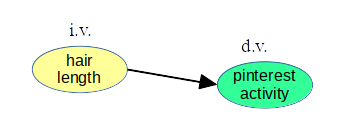
\includegraphics[width=0.6\textwidth]{hairPinterest.png}
\caption{A theory about how hair length impacts the number of times a person
logs on to pinterest each day.}
\label{fig:hairPinterest}
\end{figure}

Now of course this follicle stuff is bogus. I'm using an extreme example to
make a point. Quick, can you come up with a possible confounding factor? Yeah,
drr: \textit{gender}. It's undoubtedly true that women tend to (but don't
always) have longer hair than men, and it's undoubtedly true that
\texttt{pinterest.com} is a website that tends to appeal to (but not
exclusively to) women. And causality-wise, the arrows obviously flow from
gender, not to it: the pinterest login screen doesn't change your gender, and a
man won't turn into a woman simply by growing his hair long (although a
transgender woman might grow her hair long as a signal of her underlying gender
change.) 

Put that all together, and you get the much more plausible causal diagram in
Figure~\ref{fig:hairPinterest2}.

\begin{figure}[ht]
\centering
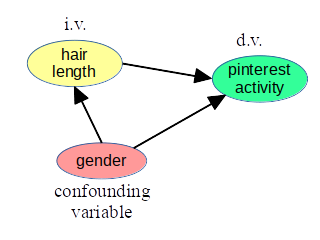
\includegraphics[width=0.6\textwidth]{hairPinterest2.png}
\caption{An alternative theory that holds that a person's gender influences
both their long-haired-ness and their pinterest-ness.}
\label{fig:hairPinterest2}
\end{figure}


\index{control (for a variable)}
\index{stratification}

Now then. Controlling for a confounding variable through stratification is done
by considering the objects of the study in \textit{groups}, comparing
\textit{only those who have the same (or similar) value for the confounding
variable.}

In this case, we would separate the men from the women in our study. Looking at
\textit{just the men}, we would ask, ``is longer hair associated with frequency
of pinterest logins?'' Then we would do the same, looking at \textit{just the
women.} Only if Python reported that both of these separate groups illustrated
such a trend would we (tentatively) conclude, ``hair length itself does play a
role in causing pinterest activity, \textit{even when controlling for
gender.}''

Do the thought experiment to see if you agree. I know the whole follicle theory
struck you as dumb (and hopefully, a little funny) to begin with. ``Of
\textit{course},'' you said to yourself, ``it's gender, not hair length, that's
drawing users to pinterest, dummy!'' But suppose we \textit{did} perform that
stratification technique, and discovered that the association actually
\textit{did} hold in both cases. Would that give it more credence in your mind?
It ought to. By stratifying, we've eliminated gender from the picture entirely,
and now we're faced with the facts that those with longer hair -- regardless of
gender -- log on to pinterest more often. 

\index{association}

Now I wrote the word ``tentatively'' a couple paragraphs ago, because there are
still some caveats. For one, we don't actually know that the causality goes in
the stated direction. Removing the gender confounder, we confirmed that there
is still an association between hair length and pinterest, but that association
might translate into a $B \rightarrow A$ phenomenon. Perhaps users who log on
to pinterest a lot see a lot of long-haired users, and (consciously or not)
decide to grow their own hair out as a result? That actually sounds more
plausible than the original silly theory. Either way, we can't confirm the
direction just by stratifying.

The other caveat is even more important, because it's more pervasive: just
because we got rid of one confounding variable doesn't mean there aren't
others. The whole ``control for a variable'' approach requires us \textit{to
anticipate in advance} what the possible confounding factors would be. This is
why I said back on p.~\pageref{smart} that this approach requires the
experimenter to be smart.

\subsection{Running a controlled experiment}

\index{controlled experiment}
\index{observational study}

The other way to deal with confounding variables is to run a \textbf{controlled
experiment} instead of an \textbf{observational study}. I jokingly said on
p.~\pageref{smart} that this option requires the experimenter to have money.
Let me explain.

% TODO: uhh...actually include the DGP chapter, as promised below.

\index{data-generating process (DGP)}
An observational study is one in which data is produced by naturally occurring
processes (we'll call them \textbf{data-generating processes}, or
\textbf{DGPs}, in a later chapter) and then collected by the researcher.
Crucially, the experimenter plays no role in influencing what any of the
variable values are, whether that be the i.v.~, the d.v.~, other related
variables, or even possible confounders. Everything just is what it is, and the
researcher is simply observing.

Now at first this sounds like the best of all possible worlds. Scientists are
supposed to be objective, and to do everything they can to avoid biasing the
results, right? True, but the sad fact is that \textit{every observational
study has potential confounding factors} and there's simply no foolproof way to
account for them all. If you \textit{knew} them all, you could potentially
account for them. But in general we don't know. It all hinges on our
cleverness, which is a bit like rolling the dice.

\index{randomization!of experimental subjects}
\index{controlled experiment}

A controlled experiment, on the other hand, is one in which \textit{the
researcher decides what the value of the i.v.~will be for each object of
study.} She normally does this randomly, which is why this technique is called
\textbf{randomization}.

Now controlled experiments bear some good news and some bad news. First, the
good news, which is incredibly good, actually: \textit{a controlled experiment
automatically eliminates \underline{every} possible confounding factor, whether
you thought of it or not.} Wow: magic! We get this boon because of how the
i.v.~works. The researcher's coin flip is the \textit{sole} determinant of who
gets which i.v.~value. That means that no other factor can be ``upstream'' of
the coin flip and influence it in any way. And this in turn nullifies all
possible confounding factors, since as you recall, a confounder must affect
both the i.v.~and the d.v.

The catch is that controlled experiments can be very expensive to run, and in
many cases can't be run at \textit{all}. Consider the barbecue example from
p.~\pageref{barbecue}. To carry out a controlled experiment, we would have to:

\begin{compactenum}
\item Recruit participants to our study, and get their informed consent.
\item Pay them some \$\$ for their trouble.
\item For each participant, flip a coin. If it comes up heads, \textit{that
person must eat barbecue three times per week for the next ten years.} If it's
tails, \textit{that person must never eat barbecue for the next ten years.}
\item At the end of the ten years, measure how many barbecuers and
non-barbecuers have cancer.
\end{compactenum}

There's a question of this even being ethical: if we suspect that eating
barbecue can cause cancer, is it okay to ``force'' participants to eat it? Even
past that point, however, there's the expense. Ask yourself: if you were a
potential participant in this experiment, how much money would you demand in
step 2 to change your lifestyle to this degree? You might love barbecue, or you
might hate it, but either way, it's a coin flip that makes your decision for
you. That's a costly and intrusive change to make.

Other scenarios are even worse, because they're downright impossible. We can't
flip coins and make (at random) half of our experimental subjects male
and the other half female. We can't (or at least, shouldn't) randomly decide
our participants' political affiliations, making one random half be Democrats
and the others Republicans. And we certainly can't dictate to the nations of
the world to emit large quantities of greenhouse gases in some years and small
quantities in others, depending on our coin flip for that year.

Bottom line: if you can afford to gather data from a controlled experiment
rather than an observational study, always choose to do so. Unfortunately, it
won't always be possible, and we'll have to rest on the uneasy assumption that
we successfully predicted in advance all the important confounding variables
and controlled for them.

\section{Spurious associations}

\index{spurious association}
\index{association!spurious}

Okay, back to Figure~\ref{fig:causalityTypes} on
p.~\pageref{fig:causalityTypes}. The other item I'd like to point out in that
table is the last one, which is called a \textbf{spurious association}. This is
written as ``$A \not\rightarrow B$,'' with the arrow crossed out. And it simply
means ``nope, none of the above: these variables actually aren't associated at
all.''

You might be scratching your head at that one. Didn't I tell you
(p.~\pageref{pythonAssociation}) that Python is smart enough to tell us
definitively whether or not two variables are associated? That was supposed to
be the easy part; the hard part was only in figuring out what \textit{causes}
that association. But now I'm saying that associations might not be
associations, and Python is powerless to know the difference!

\index{IQ}
The root cause of this state of affairs is obvious once you see it, and it has
to do with the ``how much more?'' questions from p.~\pageref{howMuchMore}.
Clearly, when we collect data, there's a ``luck of the draw'' component
ever-present. I might have data that suggests Republican voters have higher
income than Democratic voters...but it's of course possible that I just
happened to poll some richer Republicans and some poorer Democrats. Suppose I
told you I thought women were on average smarter than men, and in my random
sample the average men's IQ was 102.7 and the average woman's was 103.5. The
women's was indeed greater...but is that \textit{enough} greater? Is the
difference explainable simply by the randomness of my poll?

\index{bar}
The true answer is that we can \textit{never} know for absolute certainty,
unless we can poll the entire population. (Only if we measured the IQ of every
man and every woman on planet Earth, and took the means of both groups, could
we say which one truly had the higher mean.) But what we have to do is
essentially ``set a bar'' somewhere, and then determine whether we got over it.
We could say ``only if the average IQ difference is greater than 5 points will
we conclude that there's really a difference.''

\subsection{Setting $\alpha$}

\label{alpha}

Now the procedure for determining how high to put the ``bar'' is more
complicated and more principled than that. We don't just pick a number that
seems good to us. Instead, Python will put the bar at exactly the right height,
given the level of certainty we decide to require. Some things that influence
the placement of the bar include the sample size and how variable the data is.
The thing \textit{we} specify in the bar equation, however, is \textit{how
often we're willing to draw a false conclusion.}

\index{$\alpha$ (alpha)}
\index{alpha@alpha ($\alpha$)}

That quantity is called ``$\boldsymbol{\alpha}$'' (pronounced
``\textbf{alpha}'') and is a small number between 0 and 1. Normally we'll set
$\alpha=.05$, which means: ``Python, please tell me whether the average male
and female IQs were \textit{different enough} for me to be confident that the
difference was truly a male-vs-female thing, not just an idiosyncrasy of the
people I chose for my poll. And by the way, \textit{I'm willing to be wrong 5\%
of the time about that.}''

It seems weird at first -- why would we accept drawing a faulty conclusion 5\%
of the time? Why not 0\%? But you see, we have to put the bar somewhere. If we
said, ``I never want to think there's an association when there's not one,''
Python would respond, ``well fine, if you're so worried about it then I'll
never tell you there is one.'' There has to be some kind of criterion for
judging whether a difference is ``enough,'' and $\alpha=.05$, which is ``being
suckered only 1 in 20 times'' is the most common value for social sciences.
($\alpha=.01$ is commonly used in the physical sciences.)

So, the last entry in the Figure~\ref{fig:causalityTypes} table means ``even
though the $A$ and $B$ variables aren't \textit{really} associated at all -- if
we gathered some more $A$s and some more $B$s, we'd probably detect \textit{no}
association -- you were fooled into thinking there was one because our random
sample was a bit weird.'' There's really no way around this other than being
aware it can happen, and possibly repeating our study with a different data
set to be sure of our conclusions.


% Somewhere: .map() for recoding

\chapter[Associative arrays in Python (1 of 3)]{\huge\selectfont{Associative
arrays in Python (1 of 3)}}
\label{ch:assocArraysInPython1}

\index{associative array}
\index{Pandas package}
\index{package}
\index{importing (a package)}

Our next trick is to represent associative arrays (review
section~\ref{sec:assocArrays} if you need to) in Python. To do so, we will
use another package, which goes by the adorable name ``Pandas'':

\begin{Verbatim}[fontsize=\small,samepage=true,frame=single,framesep=3mm]
import pandas as pd
\end{Verbatim}

This code should go at the top of your first notebook cell, right under your
``\texttt{import numpy as np}'' line. The two go hand in hand.

\index{table}
\index{NumPy package}
\index{series@\texttt{Series} (Pandas)}
\index{dict@\texttt{dict} (dictionary)}

By the way, just as there were other choices besides NumPy \texttt{ndarray}s to
represent ordinary arrays, there are other choices in Python for associative
arrays. The native Python \texttt{dict} (``dictionary'') is an obvious
candidate. Because this won't work well when the data gets huge, however, and
because using Pandas now will set up our usage of tables nicely in the next
few chapters, we're going to use the Pandas \textbf{Series} data type for our
associative arrays.


\section{The Pandas \texttt{Series}}
\label{sec:creatingSeries}

\index{array!associative}
\index{key-value pair}
\index{series@\texttt{Series} (Pandas)}

A \texttt{Series} is conceptually a set of key-value pairs. The keys are
normally homogeneous, and so are the values, although the keys might be of a
different type than the values. Any of the three atomic types are permissible
for either.

\index{index@index (pl:~indices)}
\index{deep}

Somewhat confusing is that the Pandas package calls the keys ``the
\textbf{index},'' which is an overlap with the term we used for ordinary arrays
(see p.~\ref{arrayIndex}). It's not a total loss, though, since if you think
hard about it, you'll realize that in some sense, \textit{a regular array is
really just an associative array with consecutive integer keys.} Oooo, deep. If
you consider the two halves of Figure~\ref{fig:assocArraysAreArrays}, I think
you'll agree.

\begin{figure}[ht]
\centering
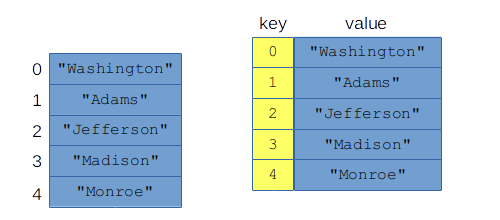
\includegraphics[width=0.9\textwidth]{assocArraysAreArrays.png}
\caption{An ordinary array, and an associative array, that represent the same
information.}
\label{fig:assocArraysAreArrays}
\end{figure}


\subsection{Creating \texttt{Series}es}

Here are a few common ways of creating a Pandas \texttt{Series} object in
memory.

\subsubsection{Way 1: create an empty \texttt{Series}}

Perhaps this first one sounds dumb, but we will indeed have occasion to start
off with an empty \texttt{Series} and then add key/value pairs to it from
there. The code is simple:

\begin{Verbatim}[fontsize=\small,samepage=true,frame=single,framesep=3mm]
my_new_series = pd.Series()
\end{Verbatim}

Voil\`{a}.

\subsubsection{Way 2: \texttt{pd.Series([], index=[])}}

As with NumPy \texttt{ndarrays}, we can explicitly list the values we want in a
new \texttt{Series}. We also have to list the \textbf{index} values (the keys).
The syntax for doing so is:

\label{marvelSeries}
\index{Marvel comics}

\begin{Verbatim}[fontsize=\small,samepage=true,frame=single,framesep=3mm]
alter_egos = pd.Series(['Hulk','Spidey','Iron Man','Thor'],
    index=['Bruce','Peter','Tony','Thor'])
\end{Verbatim}

This creates the \texttt{Series} shown in Figure~\ref{fig:Series}.

\begin{figure}[ht]
\centering
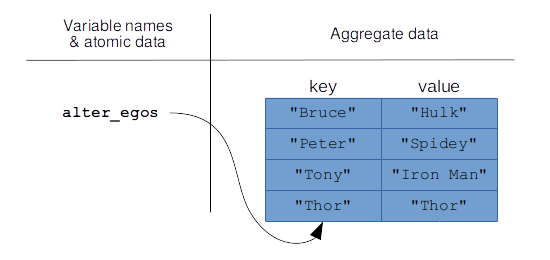
\includegraphics[width=0.8\textwidth]{Series.png}
\caption{A Pandas \texttt{Series} in memory.}
\label{fig:Series}
\end{figure}

\index{boxies (square brackets)}
\index{[]@\texttt{[]} (boxies)}
\index{bananas (parentheses)}
\index{()@\texttt{()} (bananas)}

Be careful to keep all your boxies and bananas straight. Note that both the
keys \textit{and} the values are in their own sets of boxies.

We can print (small) \texttt{Series}es to the screen to inspect their contents:

\begin{Verbatim}[fontsize=\small,samepage=true,frame=single,framesep=3mm]
print(alter_egos)
\end{Verbatim}

\begin{Verbatim}[fontsize=\small,samepage=true,frame=leftline,framesep=5mm,framerule=1mm]
Bruce        Hulk
Peter      Spidey
Tony     Iron Man
Thor         Thor
dtype: object
\end{Verbatim}

\index{type@\texttt{type()}}
\index{dtype@\texttt{.dtype} (NumPy/Pandas)}
and as we did on p.~\pageref{arrayType}, we can inquire as to both the
overarching type of \texttt{alter\_egos} and also to the kind of underlying
data it contains:

\begin{Verbatim}[fontsize=\small,samepage=true,frame=single,framesep=3mm]
print(type(alter_egos))
print(alter_egos.dtype)
\end{Verbatim}

\begin{Verbatim}[fontsize=\small,samepage=true,frame=leftline,framesep=5mm,framerule=1mm]
pandas.core.series.Series
object
\end{Verbatim}

Just as it did on p.~\pageref{dtypeRules}, the ``\texttt{object}'' here is just
a confusing way of saying ``\texttt{str}''. Don't read anything more into it
than that.

\subsubsection{Way 3: ``wrapping'' an array}

\label{wrap}
\index{dimension}

Associative arrays, and the Pandas \texttt{Series}es we've been using to
implement them, are inherently \textit{one}-dimensional data structures. This
is just like the NumPy arrays we used before. Pandas Serieses also provide a
bunch of features for manipulating, querying, computing, and even graphing
aspects of their content. It's a lot of rich stuff on top of plain-old NumPy.

\index{wrapping}

For this reason, it's common to want to create a \texttt{Series} that just
``wraps'' (or encloses) an underlying NumPy \texttt{ndarray}, and provides all
that rich stuff.

The way to do this is simple:

\begin{Verbatim}[fontsize=\small,samepage=true,frame=single,framesep=3mm]
my_numpy_array = np.array(['Ghost','Pumpkin','Vampire','Witch'])
my_pandas_enhanced_thang = pd.Series(my_numpy_array)
\end{Verbatim}

You can then treat \texttt{my\_pandas\_enhanced\_thang} as an ordinary
aggregate variable which has the more sophisticated operations of next chapter
automatically glommed on to it. The keys (index values) of this thang will
simply be the integers 0 through 3.

\subsubsection{Way 4: \texttt{pd.read\_csv()}}

Finally, there's reading data from a text flie, which as I mentioned back in
section~\ref{np.loadtxt} (p.\pageref{np.loadtxt}) is actually the most common. 
Data typically resides in sources and files external to our programming
environment, and we want to do everything we can to play ball with this open
universe.

\index{CSV@CSV (comma-separated values format)}
\index{extension@extension (filename)}
\index{filename extension}

One common data format is called \textbf{CSV}, which stands for
\textbf{comma-separated values}. Files in this format are normally named with a
``\texttt{.csv}'' extension. As the name suggests, the lines in such a file
consist of values separated by commas. For example, suppose there's a file
called \texttt{disney\_rides.csv} whose contents looked like this:

\begin{Verbatim}[fontsize=\small,samepage=true,frame=single,framesep=3mm]
Pirates of the Carribean,25
Small World,20
Peter Pan,29
\end{Verbatim}

These are the current expected wait time (in minutes) for each of these Disney
World rides at some point of the day.

\label{read_csv}
\index{read\_csv@\texttt{read\_csv()} function (Pandas)}

To read this into Python, we use the \texttt{pd.read\_csv()} function. It's a
bit awkward since it has several mandatory arguments if you want to deal with
\texttt{Series}es. Here's how it works:

\begin{Verbatim}[fontsize=\small,samepage=true,frame=single,framesep=3mm]
wait_times = pd.read_csv('disney_rides.csv', index_col=0, squeeze=True,
    header=None)
\end{Verbatim}

Most of that junk is just to memorize for now, not to fully understand. If
you're curious, \texttt{index\_col=0} tells Pandas that the first (0th) column
-- namely, the ride names -- should be treated as the \texttt{index} for the
\texttt{Series}. The \texttt{header=None} means ``there is no separate header
row at the top of the file, Pandas, so don't try to treat it like one.'' If our
\texttt{.csv} file \textit{did} have a summary row at the top, containing
labels for the two columns, then we'd skip the \texttt{header=None} part.
Finally, ``\texttt{squeeze=True}'' tells Pandas, ``since this is so skinny
anyway -- just two columns -- let's have \texttt{pd.read\_csv()} return us a
\texttt{Series}, rather than a more complex \texttt{DataFrame} object (which is
the subject of a future chapter.)''


% np.sqrt()
% np.round( , num_decimals)
% np query syntax
% np.append
% np.flip
% two kinds of sorting
% remove (by index  and by value?)

% indexing, slices

\chapter{\huge Associative arrays in Python (2 of 2)}
\label{ch:arraysInPython2}

\index{series@\texttt{Series} (Pandas)}
K, now we can create \texttt{Series}es; let's figure out what we can do with
them.

\section{Accessing individual elements}

\index{element}
\index{len@\texttt{len()}}

We can use the same \texttt{len()} function in yet a third way: to ascertain
the number of key/value pairs in a series. Using the Figure~\ref{fig:Series}
example (p.~\pageref{fig:Series}):

\begin{Verbatim}[fontsize=\small,samepage=true,frame=single,framesep=3mm]
print(len(alter_egos))
\end{Verbatim}

\begin{Verbatim}[fontsize=\small,samepage=true,frame=leftline,framesep=5mm,framerule=1mm]
4
\end{Verbatim}

\index{boxies (square brackets)}
\index{[]@\texttt{[]} (boxies)}

Accessing the value for a given key uses exactly the same syntax that NumPy
arrays used (boxies), except with the key in place of the numeric index:

\begin{Verbatim}[fontsize=\small,samepage=true,frame=single,framesep=3mm]
superhero = alter_egos['Peter']
print("Pssst...Peter is really {}.".format(superhero))
\end{Verbatim}

\begin{Verbatim}[fontsize=\small,samepage=true,frame=leftline,framesep=5mm,framerule=1mm]
Pssst...Peter is really Spidey.
\end{Verbatim}

\index{uniqueness!of keys in an associative array}

This is why it's important that the \textit{keys} of an associative array be
unique, even though the \textit{values} often aren't. If we type
``\texttt{alter\_egos[\textquotesingle Peter\textquotesingle]},'' we need to
get back one well-defined answer, not an ambiguous set of
alternatives.\footnote{Pandas, which tries to be All Things To All
People\texttrademark, will actually let you have duplicate index values in a
\texttt{Series}. What does it do if you ask for ``the'' value of
\texttt{Peter}, then, if there's more than one? It gives you back another
\textit{\texttt{Series}} of the different \texttt{Peter} superheroes. This is a
major pain, because now when you look up a value in the \texttt{Series}, you
don't know whether you'll get back a single item or another \texttt{Series},
which means you have to check to see which one it is, and then write different
code to handle the two cases...yick. Just stay far, far away. Make all your
keys unique.}

To overwrite the value for a key with a new value, just treat it as a variable
and go:

\begin{Verbatim}[fontsize=\small,samepage=true,frame=single,framesep=3mm]
alter_egos['Bruce'] = 'Batman'
print(alter_egos)
\end{Verbatim}

\begin{Verbatim}[fontsize=\small,samepage=true,frame=leftline,framesep=5mm,framerule=1mm]
Bruce      Batman
Peter      Spidey
Tony     Iron Man
Thor         Thor
dtype: object
\end{Verbatim}

This same syntax works for adding an entirely \textit{new} key/value pair as
well:

\begin{Verbatim}[fontsize=\small,samepage=true,frame=single,framesep=3mm]
alter_egos['Diana'] = 'Wonder Woman'
print(alter_egos)
\end{Verbatim}

\begin{Verbatim}[fontsize=\small,samepage=true,frame=leftline,framesep=5mm,framerule=1mm]
Bruce          Batman
Peter          Spidey
Tony         Iron Man
Thor             Thor
Diana    Wonder Woman
dtype: object
\end{Verbatim}

It's just like with ordinary variables, if you think about it. Saying
``\texttt{x=5}'' overwrites the current value of \texttt{x} if there already
\textit{is} an \texttt{x}, otherwise it creates a new variable \texttt{x} with
that value.

Finally, to outright remove a key/value pair, you use the \texttt{del}
operator:

\begin{Verbatim}[fontsize=\small,samepage=true,frame=single,framesep=3mm]
del alter_egos['Tony']
print(alter_egos)
\end{Verbatim}

\begin{Verbatim}[fontsize=\small,samepage=true,frame=leftline,framesep=5mm,framerule=1mm]
Bruce          Batman
Peter          Spidey
Thor             Thor
Diana    Wonder Woman
dtype: object
\end{Verbatim}

Bye bye, Iron Man.

\index{in place@``in place''}

Don't get mad when I tell you that all of the above operations work
\textbf{in place} on the \texttt{Series}, which is very different than some of
the ``return a modified copy'' style we've seen recently. Hence all of these
attempts are \textit{wrong}:

\begin{Verbatim}[fontsize=\small,samepage=true,frame=single,framesep=3mm]
alter_egos = del alter_egos['Tony']                   <--- WRONG!
alter_egos = alter_egos['Bruce'] = 'Batman'           <--- WRONG!
alter_egos = alter_egos['Diana'] = 'Wonder Woman'     <--- WRONG!
\end{Verbatim}

You don't ``change a value and get a new \texttt{Series}''; you just
``change it.''

\subsection{Accessing by pair number}

\index{order}

\index{iloc@\texttt{.iloc} syntax (Pandas)}

One slightly weird thing you can do with a Pandas \texttt{Series} is ignore the
key (index) altogether and instead use \textit{the number of the key/value
pair} to specify what value you want. This gives me the heebie-jeebies, because
as I explained back on p.~\pageref{assocArraysUnordered}, there really isn't
any meaningful ``order'' to the key/value pairs of an associative array. In
true All Things To All People\texttrademark~fashion, however, Pandas lets you
ask for the value of (say) ``the second'' superhero. To do so, you use the
bizarrely-named \textbf{.iloc syntax}:

\begin{Verbatim}[fontsize=\small,samepage=true,frame=single,framesep=3mm]
a_hero = alter_egos.iloc[1]
print(a_hero)
\end{Verbatim}

\begin{Verbatim}[fontsize=\small,samepage=true,frame=leftline,framesep=5mm,framerule=1mm]
Spidey
\end{Verbatim}

This is occasionally useful, so I mention it for completeness. The
\texttt{.iloc} numbers start with 0 (not 1) as is true throughout Python.

\section{Vectorized arithmetic operators}

As with NumPy \texttt{ndarrays}, you can apply arithmetic operators like
\texttt{+} and \texttt{*} to entire \texttt{Series}es at a time, which is not
only easy code to write but also runs blazing fast. But the Pandas
\texttt{Series} is even smarter than that.

\begin{figure}[ht]
\centering
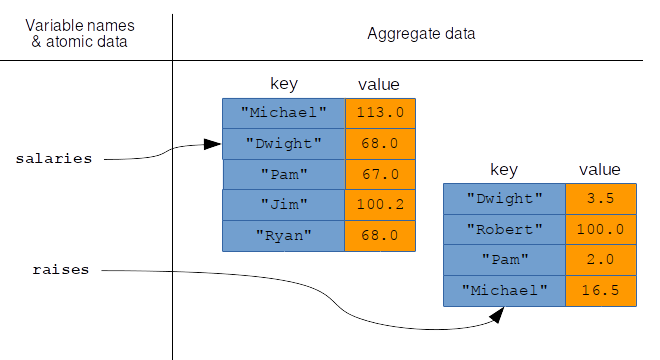
\includegraphics[width=0.9\textwidth]{vectorizedPandas.png}
\caption{Two \texttt{Series}es in memory}
\label{fig:vectorizedPandas}
\end{figure}

Consider the memory picture in Figure~\ref{fig:vectorizedPandas}. Here we have
two \texttt{Series}es, one pointed to by a \texttt{salaries} variable and the
other by \texttt{raises}, which are of different sizes and which have
overlapping, but not identical, sets of keys. What do you suppose Pandas would
do if we executed this code?

\begin{Verbatim}[fontsize=\small,samepage=true,frame=single,framesep=3mm]
new_salaries = salaries + raises
\end{Verbatim}

The answer, happily, is the smartest possible thing it could do. Pandas gets
neither confused nor stifled by the fact that the keys are in different orders
in the two \texttt{Series}es, and instead it does what you surely want:
add corresponding elements, with matching keys, and produce a new
\texttt{Series} with all of those sums.

\begin{figure}[ht]
\centering
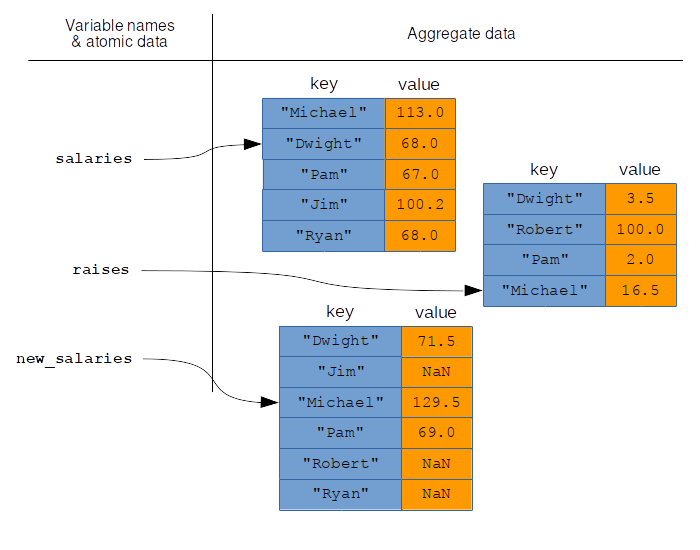
\includegraphics[width=0.8\textwidth]{vectorizedPandas2.png}
\caption{The result of \texttt{+}'ing two \texttt{Series}es that don't have all the same keys.}
\label{fig:vectorizedPandas2}
\end{figure}

The actual result in this case is in Figure~\ref{fig:vectorizedPandas2}, and
the output is here:

% salaries = pd.Series([113,68,67,100.2,68],
%   index=['Michael','Dwight','Pam','Jim','Ryan'])
% raises = pd.Series([3.5,100,2,16.5],
%   index=['Dwight','Robert','Pam','Michael'])

\begin{Verbatim}[fontsize=\small,samepage=true,frame=single,framesep=3mm]
new_salaries = salaries + raises
print(new_salaries)
\end{Verbatim}

\begin{Verbatim}[fontsize=\small,samepage=true,frame=leftline,framesep=5mm,framerule=1mm]
Dwight      71.5
Jim          NaN
Michael    129.5
Pam         69.0
Robert       NaN
Ryan         NaN
dtype: float64
\end{Verbatim}

\index{nan@\texttt{NaN} (``not a number'')}
\index{missing value}

Convince yourself that \texttt{Dwight}'s \$68,000 salary got added to his
\$3,500 raise, and that \texttt{Michael}'s \$113,000 was added to \$16,500,
\textit{etc.}

Don't get freaked out by those \texttt{NaN} entries just yet. The special value
``\textbf{NaN}'' stands for ``\textbf{not a number},'' and basically means that
Pandas has to throw up its hands in that case. And with good cause.
\texttt{Jim} has a current salary of \$100,200 in the first \texttt{Series},
but has no value at all in the second one (no raise for Jim this year? Haven't
decided what his raise will be yet? Something else?) and so Pandas shrugs and
says ``dunno.'' We say that the \texttt{Jim} entry in the
\texttt{new\_salaries} \texttt{Series} is a \textbf{missing value}. The same is
true for \texttt{Robert} and \texttt{Ryan}, each of whom was present in only
one of the two operands.

Now I know what you're thinking: ``can't Pandas just assume the salary and/or
raise is 0 if there's a missing one?'' The answer is that yes it can, but it
won't do so unless you give the go-ahead. Pandas is being cautious here, and
doesn't want to introduce errors into your data stream by false assumptions.
(Maybe in your company, for instance, there's a default entry-level salary that
every employee receives who's unspecified in the \texttt{salary}
\texttt{Series}. Or maybe the yearly raise is always assumed to be a flat 2.5\%
cost-of-living raise unless explicitly specified.)

\index{add@\texttt{add()} function (Pandas)}
\index{sub@\texttt{sub()} function (Pandas)}
\index{mul@\texttt{mul()} function (Pandas)}
\index{div@\texttt{div()} function (Pandas)}

If we do want Pandas to assume a certain default value, we have to change
tactics a bit and go with the \texttt{add()} function (or \texttt{sub()},
\texttt{mul()}, or \texttt{div()}):

\begin{Verbatim}[fontsize=\small,samepage=true,frame=single]
new_salaries = pd.Series.add(salaries, raises, fill_value=0)
print(new_salaries)
\end{Verbatim}

\begin{Verbatim}[fontsize=\small,samepage=true,frame=leftline,framesep=5mm,framerule=1mm]
Dwight      71.5
Jim        100.2
Michael    129.5
Pam         69.0
Robert     100.0
Ryan        68.0
dtype: float64
\end{Verbatim}

The \texttt{fill\_value} argument is the important one here: it specifies what
default value to use if one of the addends is missing a key from the other. Now
the result is as in Figure~\ref{fig:vectorizedPandas3}. You can, of course,
choose a \texttt{fill\_value} other than zero, if you wish.

\begin{figure}[ht]
\centering
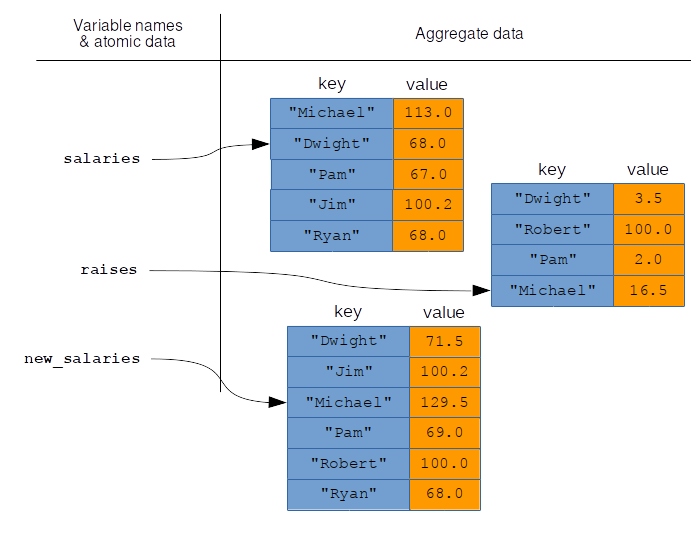
\includegraphics[width=0.8\textwidth]{vectorizedPandas3.png}
\caption{Using \texttt{add()} instead, and passing a \texttt{fill\_value}.}
\label{fig:vectorizedPandas3}
\end{figure}

As with NumPy arrays, we can add (or subtract, or multiply, ...) a single
atomic value to a series as well:

\begin{Verbatim}[fontsize=\small,samepage=true,frame=single,framesep=3mm]
cost_of_living_increase = salaries * .025
print(cost_of_living_increase)
\end{Verbatim}

\begin{Verbatim}[fontsize=\small,samepage=true,frame=leftline,framesep=5mm,framerule=1mm]
Michael    2.825
Dwight     1.700
Pam        1.675
Jim        2.505
Ryan       1.700
dtype: float64
\end{Verbatim}

\begin{Verbatim}[fontsize=\small,samepage=true,frame=single,framesep=3mm]
salaries = salaries + cost_of_living_increase
print(salaries)
\end{Verbatim}

\begin{Verbatim}[fontsize=\small,samepage=true,frame=leftline,framesep=5mm,framerule=1mm]
Michael    115.825
Dwight      69.700
Pam         68.675
Jim        102.705
Ryan        69.700
dtype: float64
\end{Verbatim}

It can sometimes be useful to do string concatenation as well, for instance if
we had employee first names and last names in two \texttt{Series}es with their
employee ID as the index:

\begin{Verbatim}[fontsize=\small,samepage=true,frame=single,framesep=3mm]
firsts = pd.Series(['Hannibal', 'Clarice', 'Multiple', 'Buffalo'],
    index=[666, 1993, 47, 988])
lasts = pd.Series(['Starling', 'Crawford', 'Lecter', 'Bill', 'Miggs'],
    index=[1993, 1650, 666, 988, 47])
print(firsts + " " + lasts)
\end{Verbatim}

\begin{Verbatim}[fontsize=\small,samepage=true,frame=leftline,framesep=5mm,framerule=1mm]
47        Multiple Miggs
666      Hannibal Lecter
988         Buffalo Bill
1650                 NaN
1993    Clarice Starling
dtype: object
\end{Verbatim}

\section{Copying \texttt{Series}es}

\section{Sorting \texttt{Series}es}
\index{in place}

\section{Concatenating and combining}

\section{Queries}

These functions are all summarized in Figure~\ref{fig:handySeries}.

\setlength\extrarowheight{5pt}

\begin{figure}[ht]
\centering
\begin{tabular}{c|p{3.3in}}
Function & Description \\
\hline

\texttt{len(}\textsl{arr}\texttt{)} & Get the number of elements in the array \textsl{arr}. \\

\textsl{arr}\texttt{[17]} & Get a specific element's value from the array \textsl{arr}. \\

\textsl{arr}\texttt{[8] =} (\textsl{something}) & Set a specific element of the array \textsl{arr}. \\

\textsl{arr} \texttt{+ 91} & Add a value to each element of \textsl{arr},
yielding a new array. (Also works with \texttt{-}, \texttt{*}, \texttt{/},
\textit{etc.}) \\

\textsl{arr1} \texttt{+} \textsl{arr2} & Add each pair of values in two arrays,
yielding a new array. (Also works with \texttt{-}, \texttt{*}, \texttt{/},
\textit{etc.}) \\

\textsl{arr1} = \textsl{arr2} & Make \textsl{arr1} point to the same data that
\textsl{arr2} points to. (\textit{Not} a copy!)\\

\textsl{arr1} = \textsl{arr2}\texttt{.copy()} & Make \textsl{arr1} point to a
new, independent copy of \textsl{arr2}. \\

\textsl{arr}\texttt{.sort()} & Sort the array \textsl{arr} \textbf{in place}. (Numerical or
alphabetical, depending on the \texttt{.dtype}.) \\

\texttt{np.sort(}\textsl{arr}) & Return a new array with the sorted elements
of \textsl{arr}. (Numerical or alphabetical, depending on the \texttt{.dtype}.)
\\

\texttt{np.append(}\textsl{arr}, \textsl{elem}\texttt{)} &
    Return a new array with \textsl{elem} tacked on to the end. \\

\texttt{np.append(}\textsl{arr1}, \textsl{arr2}\texttt{)} &
    Return a new array with the two arrays \textsl{arr1} and \textsl{arr2} concatenated. \\

\texttt{np.insert(}\textsl{arr}, \textsl{ind}, \textsl{val}\texttt{)} &
    Return a new array with the new value \textsl{val} inserted into position \textsl{ind} of \textsl{arr}. \\

\texttt{np.delete(}\textsl{arr}, \textsl{ind}\texttt{)} &
    Return a new array with the element at index \textsl{ind} removed from \textsl{arr}. \\

\texttt{np.flip(}\textsl{arr}\texttt{)} &
    Return a new array with \textsl{arr} in reverse order. \\
\end{tabular}
\bigskip
\caption{Handy functions, methods, and operators for Pandas \texttt{Series}es.}
\label{fig:handySeries}
\end{figure}


\chapter[Tables in Python (1 of 3)]{\huge\selectfont{Tables in Python (1 of
3)}}

\label{dataframes}

\index{table}
\index{DataFrame@\texttt{DataFrame} (Pandas)}

The third of our three aggregate data types from waaaay back in
Chapter~\ref{ch:aggregateData} was the \textbf{table}. Don't worry: we haven't
forgotten about him. In this chapter, we'll implement him by means of the
Pandas \texttt{DataFrame}, the most important data type in this entire book.

\section{Reading a \texttt{DataFrame} from a \texttt{.csv} file}

\index{CSV@CSV (comma-separated values format)}

Unlike NumPy arrays and Pandas \texttt{Series}es, which we learned several
different ways to create, we're only going to learn one way to create a
\texttt{DataFrame}. That's because \texttt{DataFrame}s are normally big enough
that it's just too tedious to ever type them in manually. Instead, we'll read
them from an external source; namely, a \texttt{.csv} file.

\index{read\_csv@\texttt{read\_csv()} function (Pandas)}
\index{davieses@\texttt{davieses}}

We'll actually use the same \texttt{read\_csv()} function that we used in
section~\ref{read_csv} (p.~\pageref{read_csv}), although oddly, this time we
won't need to specify as many arguments. Let's say we have a
``\texttt{davieses.csv}'' file with these contents:

\index{file!\texttt{.csv}}

\begin{Verbatim}[fontsize=\small,samepage=true,frame=lines,framesep=3mm]
person,age,gender,height,instrument
Dad,50,M,73,piano
Mom,49,F,66,flute
Lizzy,19,F,63,guitar
TJ,18,M,71,trombone
Johnny,15,M,69,euphonium
\end{Verbatim}

We can read it into a \texttt{DataFrame} with this code:

\begin{Verbatim}[fontsize=\small,samepage=true,frame=single,framesep=3mm]
my_first_data_frame = pd.read_csv("davieses.csv").set_index('person')
print(my_first_data_frame)
\end{Verbatim}
\vspace{-.2in}

\begin{Verbatim}[fontsize=\small,samepage=true,frame=leftline,framesep=5mm,framerule=1mm]
        age gender  height instrument
person                               
Dad      50      M      73      piano
Mom      49      F      66      flute
Lizzy    19      F      63     guitar
TJ       18      M      71   trombone
Johnny   15      M      69  euphonium
\end{Verbatim}

\index{header row (of a \texttt{.csv} file)}
\index{row (of a table)}

A couple things. First, you may have noticed that the \texttt{davieses.csv}
file had a ``header'' row. This means that the first line of the file is not
like the others: instead of containing information on a specific family member,
it contains the \textit{kind} of information for \textit{every} family member.
It looked like this:

\vspace{-.1in}
\begin{center}
\texttt{person,age,gender,height,instrument}
\end{center}
\vspace{-.1in}

\index{column (of a table)}
\index{metadata}

and you'll notice that these words (except for the first one; more on that in a
moment) became the \textit{column names} when we imported the data. This sort
of information, by the way, is called ``\textbf{metadata},'' a geeky-sounding
word that basically means ``data about data.'' If ``Lizzy plays the guitar'' is
a piece of data, then ``family members play instruments'' is a piece of
\textit{meta}data.

\index{read\_csv@\texttt{read\_csv()} function (Pandas)}
\index{set\_index@\texttt{set\_index()} method (Pandas)}

Second, don't miss the ending I tacked on to the \texttt{read\_csv()} line,
where I called the \texttt{.set\_index()} method on the \texttt{DataFrame}.
This tells Pandas that one of the columns in the \texttt{DataFrame} should be
designated as the \textbf{index} (or the \textbf{keys}).

\index{uniqueness!of the values in a \texttt{DataFrame} index}

Back on p.~\pageref{tablesHaveNoKey} I asserted that unlike associative arrays,
tables didn't have keys. And that's true of the general ``table'' concept. But
Pandas designed their \texttt{DataFrame}s to behave in the same way as their
\texttt{Series}es: one uniquely-valued column will be used to identify each
row.

\index{Foreman, George}
\index{George}

This choice is usually easy; if you glance back to Figure~\ref{fig:table}
(p.~\pageref{fig:table}), we'd probably want to choose the \textsf{screenname}
as the index (although a case could be made for the \textsf{real name} column
instead). For the table in Figure~\ref{fig:aggregateMemory}
(p.~\pageref{fig:aggregateMemory}), it would be the \textsf{item} column. In
the \texttt{DataFrame} we just created above, obviously \texttt{person} is the
correct choice -- it's the only one sure to be unique.\footnote{With apologies
to boxing legend George Foreman, who named all four of his sons ``George.''}

Anyway, designating a column as the index in this way sort of removes it from
the other, ``ordinary'' columns. In the output, above, you may notice that the
word ``\texttt{person}'' is printed somewhat lower than the other column names
are. It turns out that if we want to talk about the index column specifically,
we'll need to use a slightly different technique than we do for the other
columns. More on that next chapter.

\section{Missing values}

Let's change the example to a different family, and a slightly bigger
\texttt{DataFrame}. The ``\texttt{simpsons.csv}'' file is reproduced below. Do
you notice anything odd about it?

\index{simpsons@The Simpsons}
\index{Santa's Little Helper}
\index{file!\texttt{.csv}}

\begin{Verbatim}[fontsize=\small,samepage=true,frame=lines,framesep=3mm]
name,species,age,gender,fave,IQ,hair,salary
Homer,human,36,M,beer,74,,52000
Marge,human,34,F,helping others,120,stacked tall,
Bart,human,10,M,skateboard,90,buzz,
Lisa,human,8,F,saxophone,200,curly,
Maggie,human,1,F,pacifier,100,curly,
SLH,dog,4,M,,,shaggy,
\end{Verbatim}

\index{double comma@``double comma''}

What I mean is the positioning of some of the commas. The sharp-eyed reader
will see a ``double comma'' in Homer's row. Even a dull-eyed reader will notice
several commas in a row in SLH's\footnote{The Simpson's dog was named ``Santa's
Little Helper.''} row. And nearly \textit{every} row (the exception being
Homer's) \textit{ends} with a comma, which just looks messed up.

\index{missing value}

This weird punctuation implies the existence of \textbf{missing values}, which
means just what it sounds like: there's simply no data for certain columns of 
certain rows. Homer doesn't have a ``\texttt{hair}'' value, no one \textit{but}
Homer has a ``\texttt{salary}'' value, and SLH is missing all kinds of stuff.

When we read this into a Pandas \texttt{DataFrame} a la:

\begin{Verbatim}[fontsize=\small,samepage=true,frame=single,framesep=3mm]
simpsons = pd.read_csv("simpsons.csv").set_index('name')
\end{Verbatim}

the result looks like this:

\begin{Verbatim}[fontsize=\small,samepage=true,frame=leftline,framesep=5mm,framerule=1mm]
       species  age gender            fave     IQ          hair   salary
name                                                                    
Homer    human   36      M            beer   74.0           NaN  52000.0
Marge    human   34      F  helping others  120.0  stacked tall      NaN
Bart     human   10      M      skateboard   90.0          buzz      NaN
Lisa     human    8      F       saxophone  200.0         curly      NaN
Maggie   human    1      F        pacifier  100.0         curly      NaN
SLH        dog    4      M             NaN    NaN        shaggy      NaN
\end{Verbatim}

\index{nan@\texttt{NaN} (``not a number'')}

The missing values come up as \texttt{NaN}'s, the same value you may remember
from p.~\pageref{NaN}. The monker ``not a number'' makes sense for the
\texttt{salary} case, although I think it's a bit weird for Homer's
\texttt{hair} (not a number? is hair \textit{supposed} to be a number?...)
At any rate, we can expect that this will be the case for many real-world data
sets.

\index{objects (of a study)}

``Missing'' can mean quite a few subtly different things, actually. Maybe it
means that the value for that object of study was collected, but lost. Maybe it
means it was never collected at all. Maybe it means that variable doesn't
really make \textit{sense} for that object, as in the case of a dog's IQ.
Ultimately, if we want to use the other values in that row, we'll have to come
to terms with what the missing values \textit{mean}. For now, let's just learn
a couple of coarse ways of dealing with them.

\index{dropna@\texttt{.dropna()} method (Pandas)}

One (sometimes) handy method is \texttt{.dropna()}. If you call it, it will
return a modified copy of the \texttt{DataFrame} in which any row with an
\texttt{NaN} is removed. This turns out to be overkill in the Simpson's case,
though:

\begin{Verbatim}[fontsize=\small,samepage=true,frame=single,framesep=3mm]
print(simpsons.dropna())
\end{Verbatim}
\vspace{-.2in}

\begin{Verbatim}[fontsize=\small,samepage=true,frame=leftline,framesep=5mm,framerule=1mm]
Empty DataFrame
Columns: [species, age, gender, fave, IQ, hair, salary]
Index: []
\end{Verbatim}

In other words, nothing's left. (Every row had at least one \texttt{NaN} in
it, so nothing survived.)

We could pass an optional argument to \texttt{.dropna()} called
``\texttt{how}'', and set it equal to \texttt{"all"}: in this case only rows
with \textit{all} \texttt{NaN} values are removed. Sometimes that's
``underkill,'' as in our Simpson's example: after all, none of the rows are
\textit{entirely} \texttt{NaN}'s, so calling \texttt{.dropna(how="all")}
would leave everything intact.

\index{fillna@\texttt{.fillna()} method (Pandas)}
\index{default value}

Another option is the \texttt{.fillna()} method, which takes a ``default
value'' argument: any \texttt{NaN} value is replaced with the default in the
modified copy returned. Let's try it with the string \texttt{"none"} as the
default value:

\begin{Verbatim}[fontsize=\small,samepage=true,frame=single,framesep=3mm]
print(simpsons.fillna("none"))
\end{Verbatim}
\vspace{-.2in}

\begin{Verbatim}[fontsize=\small,samepage=true,frame=leftline,framesep=5mm,framerule=1mm]
       species  age gender            fave    IQ          hair salary
name                                                                 
Homer    human   36      M            beer    74          none  52000
Marge    human   34      F  helping others   120  stacked tall   none
Bart     human   10      M      skateboard    90          buzz   none
Lisa     human    8      F       saxophone   200         curly   none
Maggie   human    1      F        pacifier   100         curly   none
SLH        dog    4      M            none  none        shaggy   none
\end{Verbatim}

This is possibly useful, but in this case it's not a perfect fit because
different columns call for different defaults. The \texttt{fave} and
\texttt{hair} columns could well have ``\texttt{none}'' (indicating no
favorite thing, and no hair, respectively) but we might want the default
\texttt{salary} to be 0. The way to accomplish that is to change the individual
columns of the \texttt{DataFrame}. Here goes:

\begin{Verbatim}[fontsize=\small,samepage=true,frame=single,framesep=3mm]
simpsons['salary'] = simpsons['salary'].fillna(0)
simpsons['IQ'] = simpsons['IQ'].fillna(100)
simpsons['hair'] = simpsons['hair'].fillna("none")
print(simpsons)
\end{Verbatim}
\vspace{-.2in}

\begin{Verbatim}[fontsize=\small,samepage=true,frame=leftline,framesep=5mm,framerule=1mm]
       species  age gender            fave     IQ          hair   salary
name                                                                    
Homer    human   36      M            beer   74.0          none  52000.0
Marge    human   34      F  helping others  120.0  stacked tall      0.0
Bart     human   10      M      skateboard   90.0          buzz      0.0
Lisa     human    8      F       saxophone  200.0         curly      0.0
Maggie   human    1      F        pacifier  100.0         curly      0.0
SLH        dog    4      M             NaN  100.0        shaggy      0.0
\end{Verbatim}

Here we've assumed that the default IQ, for someone who hasn't taken the test,
is 100 (the average). I left the \texttt{NaN} in \texttt{fave} as is, since
that seemed appropriate.

\begin{samepage}
By the way, that code is actually more than it may appear at first. When we
execute a line like:

\vspace{-.1in}
\begin{center}
\texttt{simpsons[\textquotesingle salary\textquotesingle] =
simpsons[\textquotesingle salary\textquotesingle].fillna(0)}
\end{center}
\vspace{-.1in}
\end{samepage}

we're really saying ``please \textit{replace} the \texttt{salary} column of the
\texttt{simpsons} \texttt{DataFrame} with a new column. That new column should
be -- wait for it -- the existing \texttt{salary} column but with zeros
replacing the \texttt{NaN}'s.''

We'll see many more cases of changing \texttt{DataFrame} columns wholesale in
the following chapters.

\section{Removing rows/columns}

Finally, there are times when after reading a \texttt{.csv} file into a
\texttt{DataFrame}, you want to manually delete certain rows and/or columns
that are not going to be of interest.


\begin{samepage}

\index{drop@\texttt{.drop()} method (Pandas)}
\index{Santa's Little Helper}
The easiest syntax for deleting a row (say, Santa's Little Helper) is:

\begin{Verbatim}[fontsize=\small,samepage=true,frame=single,framesep=3mm]
simpsons = simpsons.drop('SLH')
\end{Verbatim}
\end{samepage}

The \texttt{.drop()} method takes the index of the undesired row as an
argument, Like most of the methods we've seen so far, it returns a modified
copy of the \texttt{DataFrame} it's called on, so you have to reassign this to
the original variable (or use the \texttt{inplace=True} argument).

\index{boxies (square brackets)}
\index{[]@\texttt{[]} (boxies)}

\begin{samepage}
You can even delete multiple rows at the same time by enclosing the undesired
indices in boxies:

\begin{Verbatim}[fontsize=\small,samepage=true,frame=single,framesep=3mm]
simpsons = simpsons.drop(['Homer','Marge','SLH'])
\end{Verbatim}
\end{samepage}

\begin{samepage}

\index{del operator@\texttt{del} operator (Pandas)}
Deleting a column is even more common, since many tables ``in the wild'' have
many, many columns, only a few of which you may care about in your analysis.
You can whack one entirely with the \texttt{del} operator, just like we did for
\texttt{Series}es (p.~\pageref{delOp}):

\begin{Verbatim}[fontsize=\small,samepage=true,frame=single,framesep=3mm]
del simpsons['IQ']
\end{Verbatim}
\end{samepage}


\backmatter
\printindex

\end{document}
